%https://books.google.cz/books?id=DiFMPmXSsLUC&pg=SA6-PA15&lpg=SA6-PA15&dq=Varshni+1967&source=bl&ots=hBJXnBqrHH&sig=WuCbtLj6FUIWMr09BP1LkBR-2cc&hl=cs&sa=X&ved=0ahUKEwi5mPz5lL_ZAhUGEVAKHRiaAOIQ6AEIXDAH#v=onepage&q=Varshni%201967&f=false

\chapter{InGaAsSb/GaAs/GaP QDs for Flash memories}\label{chap:TUB_QD}

%The direct-band gap semiconductor InGaAs represents the basic of the active area of a multitude of commercial photonic devices
%Optical emitters are one of the key components of optoelectronics and photonics. Despite the considerable progress in light emitting technology in visible spectral range during the last decades, the implementation of efficient light emitters on silicon remains a challenge. 
Today's market of computer memories is divided mainly between two kinds of memories, i.~e., the dynamical random access memory (DRAM)~\citep{waser_2003} and the flash memory~\citep{Pavan_1997}. The DRAM is fast but volatile, which means that the information must be refreshed within every tens milliseconds. On the other hand flash memory is a non-volatile memory with a storage time of more than ten years without any power consumption, however, it suffers from a slow write time of several microseconds. Semiconductor memory community is seeking for a memory based on the advantages of both previous types, which would combine the fast write/read speed with long storage time. Different approaches toward that goal are studied at the moment, such as FeRAM, MRAM or PCRAM, etc.~\citep{Burr_IBM2008}.

One of the promising options to combine fast write speed and long storage time is the use of QD-Flash~\citep{Geller_APL2008_QDFlash}, a memory based on self-organized quantum dots (QDs) fabricated from III-V materials. These nano-objects can be prepared by Stranski-Krastanov growth mode and due to a variety of material band structure engineering its band-offsets and barriers can be tuned in contrast to the fixed SiO$_2$ barriers in the current Flash memories.\\
%
\indent Storage of information is always a non-equilibrium situation, which is lost after a certain time. In the QD-based memory this process is limited by certain time of thermal emission only. The storage time for various materials based on either electron~\citep{Anand_apl1995_elflash,Nowozin_2013_sum} or hole~\citep{GellerPRB, stracke_apl2012_qdflash_GaP,Nowozin_2013_sum} storages were studied. The energy levels of confined holes in a QD are much more favourably confined than those of electrons owing to their larger effective mass, therefore, at least one order of magnitude more holes can be stored in a given volume than electrons. \\
%
\indent One of the suitable systems for realization of long storage time QD-Flash are heterostructures grown on GaP substrate. For In$_{0.25}$Ga$_{0.75}$As/GaAs/GaP the storage time of 3~$\mu$s was measured at room temperature~\citep{stracke_apl2012_qdflash_GaP}, which is insufficient for memory usage, however, it is already three orders higher than the time for a typical representative of III-V QDs from InGa/GaAs~\citep{GellerPRB}. Longer storage time can be expected in the GaSb/GaP system, due to higher localization energy. Several pioneering studies have been reported for GaSb/GaP system, where the storage time is predicted in a range 1 and $10^5$ years with 8-band $\mathbf{k\cdot p}$ calculations~\citep{Bimberg_proceedingSPIE}, however the experimentally observed times were not larger than 3.9~days~\citep{Bonato_pssolidi_GaSbonGaP}.\\%  Moreover, the storage time for GaSb/GaP heterostructure was predicted in a range 1 and $10^5$ years with 8-band $\mathbf{k\cdot p}$ calculations~\citep{Bimberg_proceedingSPIE}.\\
%
\indent The use of structures grown on GaP substrate has another benefit besides other III-V semiconductors, where crystalline defects are generated during the III-V/Si heteroepitaxy. It was proposed to use pseudomorphic GaP/Si substrate benefiting from the low lattice mismatch between GaP and Si (0.37~\% at 300~K) to avert the formation of these defects~\citep{Beyer_jap2013,Grassman_apl2013, Lin_jcg2013}. Hence, the GaP-based heterostructures can be implemented in defect-free quality on Si chips.

In this chapter, we follow several previous experimental works which investigated {(In,Ga)As/GaP} QDs. InAs/GaP QDs have first been reported in Refs.~\citep{Leon_apl1998, guo_solidi2009}, but efficient PL was not achieved because of the plastic relaxation due to the large lattice mismatch (11.2\%). Then Futchi et al.~\citep{Fuchi_physicaE2004} measured PL up to 77~K on InGaAs/GaP QDs and pointed to the issue of In composition and dominant role of In amount was demonstrated via calculations~\citep{Fukami_solodi2011}. Rivoire et al.~\citep{Rivoire_prb2012} claimed a single dot emission of type-I In$_{0.5}$Ga$_{0.5}$As/GaP QDs, subsequently, the structural and emission properties were studied~\cite{Stracke_apl2014, Sala_apl2016}. To initiate the Stranski-Krastanov growth mode of In$_x$Ga$_{1-x}$As QDs on GaP, the GaP surfaces need to be covered by thin layer of GaAs prior to In$_x$Ga$_{1-x}$As deposition~\citep{stracke_apl2012_qdflash_GaP}.
%
%
% konec korekci PK
%
%
We investigate a set of samples with In$_{1-x}$Ga$_{x}$As$_y$Sb$_{1-y}$/GaAs/GaP QDs with GaAs thickness of 5~ML by centered around the energy of 1.8~eV, where emission from QDs is expected. We study PL of these samples as function of excitation power and temperature. The dynamics of optical transitions in the studied ensemble is examined by time-resolved PL (TRPL).


\section{In$_{1-x}$Ga$_{x}$As$_y$Sb$_{1-y}$/GaAs/GaP QDs samples}
The samples were grown on GaP(001) substrate by metalorganic vapor phase epitaxy (MOVPE) in Stranski-Krastanov mode in a horizontal Aixton 200 reactor using H$_2$ as carrier gas at Technische Universität Berlin~\citep{Sala_apl2016}. \\
%
\indent The growth starts with 250~nm GaP buffer layer followed by 20~nm AlGaP barrier and 150~nm GaP at the temperature of 750~$^\circ$C. Subsequently the temperature is reduced to 500~$^\circ$C for the following steps: (i) growth of a thin GaAs interlayer (5~ML) for all studied samples, (ii) for samples which we call S$_\mathrm{with}$ and S$_\mathrm{cap}$ a short Sb-flush is applied by supplying the triethyl-antimony for two and one second, respectively, at input flux of $2.6~\mu\mathrm{mol/min}$, (iii) In$_{1-x}$Ga$_{x}$As$_y$Sb$_{1-y}$ QDs growth, (iv) GaSb cap in case of sample S$_\mathrm{cap}$ (v) growth interruptions (GRI) for 1~s, and finishing the structure by GaP capping layer of 6~nm thickness. Finally, samples are heated to 620~$^\circ$C to grow 50~nm thick GaP layer. The samples are depicted in Fig.~\ref{fig:TUstructure} and their differences and labels are summarized in Tab.~\ref{tab:samples}.
\begin{figure}
	\centering
	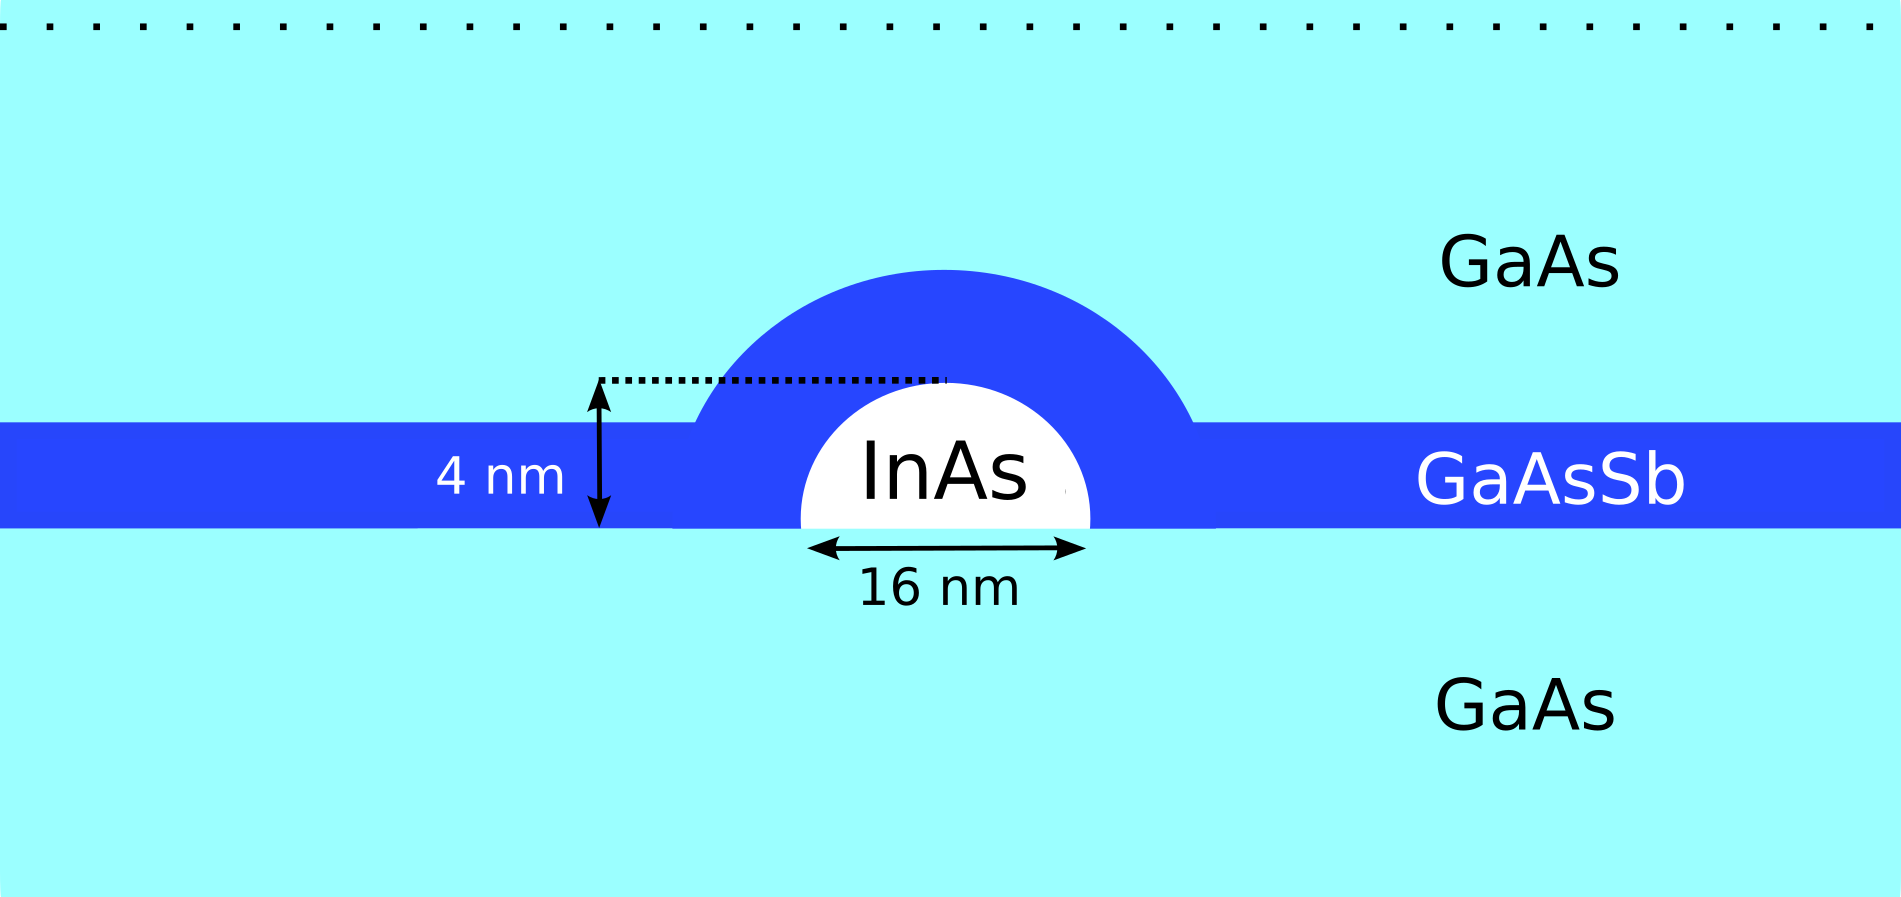
\includegraphics[width=1\linewidth]{/TEM/structure}
	\caption{Studied set of samples, $S_\mathrm{w/o}$ represents structure without QDs, $S_\mathrm{with}$ and $S_\mathrm{cap}$ are samples with In$_{1-x}$Ga$_{x}$As$_y$Sb$_{1-y}$ QDs, $S_\mathrm{cap}$ is, moreover, GaSb capped. }
	\label{fig:TUstructure}
\end{figure}

\begin{table}
	\centering
	\caption{Labels and studied sample differences.}
	%\begin{tabularx}{0.9\textwidth}{ccccc}
	\begin{tabularx}{0.95\textwidth}{ccl}
		\toprule

		%growing name & our marking& \multicolumn{3}{c}{specification}\\ 
		sample name & label& \multicolumn{1}{c}{specification}\\ 		
		\midrule
		\midrule
		%TU 12027& $S_\mathrm{w/o}$ & 5ML GaAs& &\\
		TU 12027& S$_\mathrm{w/o}$ & 5ML GaAs\\
		%TU 12040& $S_\mathrm{with}$ & 5ML GaAs,& 0.51ML In$_{1-x}$Ga$_{x}$As$_y$Sb$_{1-y}$&\\
		TU 12040& S$_\mathrm{with}$ & 5ML GaAs, 0.51~ML In$_{1-x}$Ga$_{x}$As$_y$Sb$_{1-y}$ QDs\\
		%TU 12021 & $S_\mathrm{cap}$ & 5ML GaAs,& 0.51ML In$_{1-x}$Ga$_{x}$As$_y$Sb$_{1-y}$,& GaSb cap\\
		TU 12021 & S$_\mathrm{cap}$ & 5ML GaAs, 0.51~ML In$_{1-x}$Ga$_{x}$As$_y$Sb$_{1-y}$ QDs, GaSb cap\\
		\bottomrule
	\end{tabularx}\label{tab:samples}
\end{table}

% http://nano.ceitec.cz/high-resolution-scanning-transmission-electron-microscope-fei-titan-themis-60-300-cubed/

We have studied the material composition of the sample S$_\mathrm{cap}$ by transmission electronic microscopy (TEM) with an add-on energy-dispersive X-ray (EDX) detector (SUPER-X EDX detector was used). These measurements were performed at the high resolution TEM FEI Titan Themis at CEITEC Brno. The TEM image of the whole sample and EDX emission spectrum are attached in appendix~\ref{chapter:appendix_TEM}.

In Fig.~\ref{fig:TEM}, cross-sectional TEM micrograph and graphs from parallel measured EDX for sample S$_\mathrm{cap}$ are presented. EDX spectrum is collected along the orange dashed line and averaged in the yellow boundary area. In the atomic fraction graph we show material composition in the sample as a function of horizontal position for all constituents (Ga, P, As, In, Sb). In the range between 30 and 40~nm in the cut In, As and Sb composition (elements, which are expected only in QDs area) dramatically in comparison with the concentration of 0.8~\% seen in the remainder of the sample. In the same range, we can see a decrease in phosphorus concentration at the expense of GaP. The layer where In concentration is higher than 0.8~\% we regard as QD area and its thickness is found to be of 5.8~nm with truncated-pyramid shape QDs with a base length of about 15~nm and a height of 2.5~nm. 
\begin{figure}
	\centering
	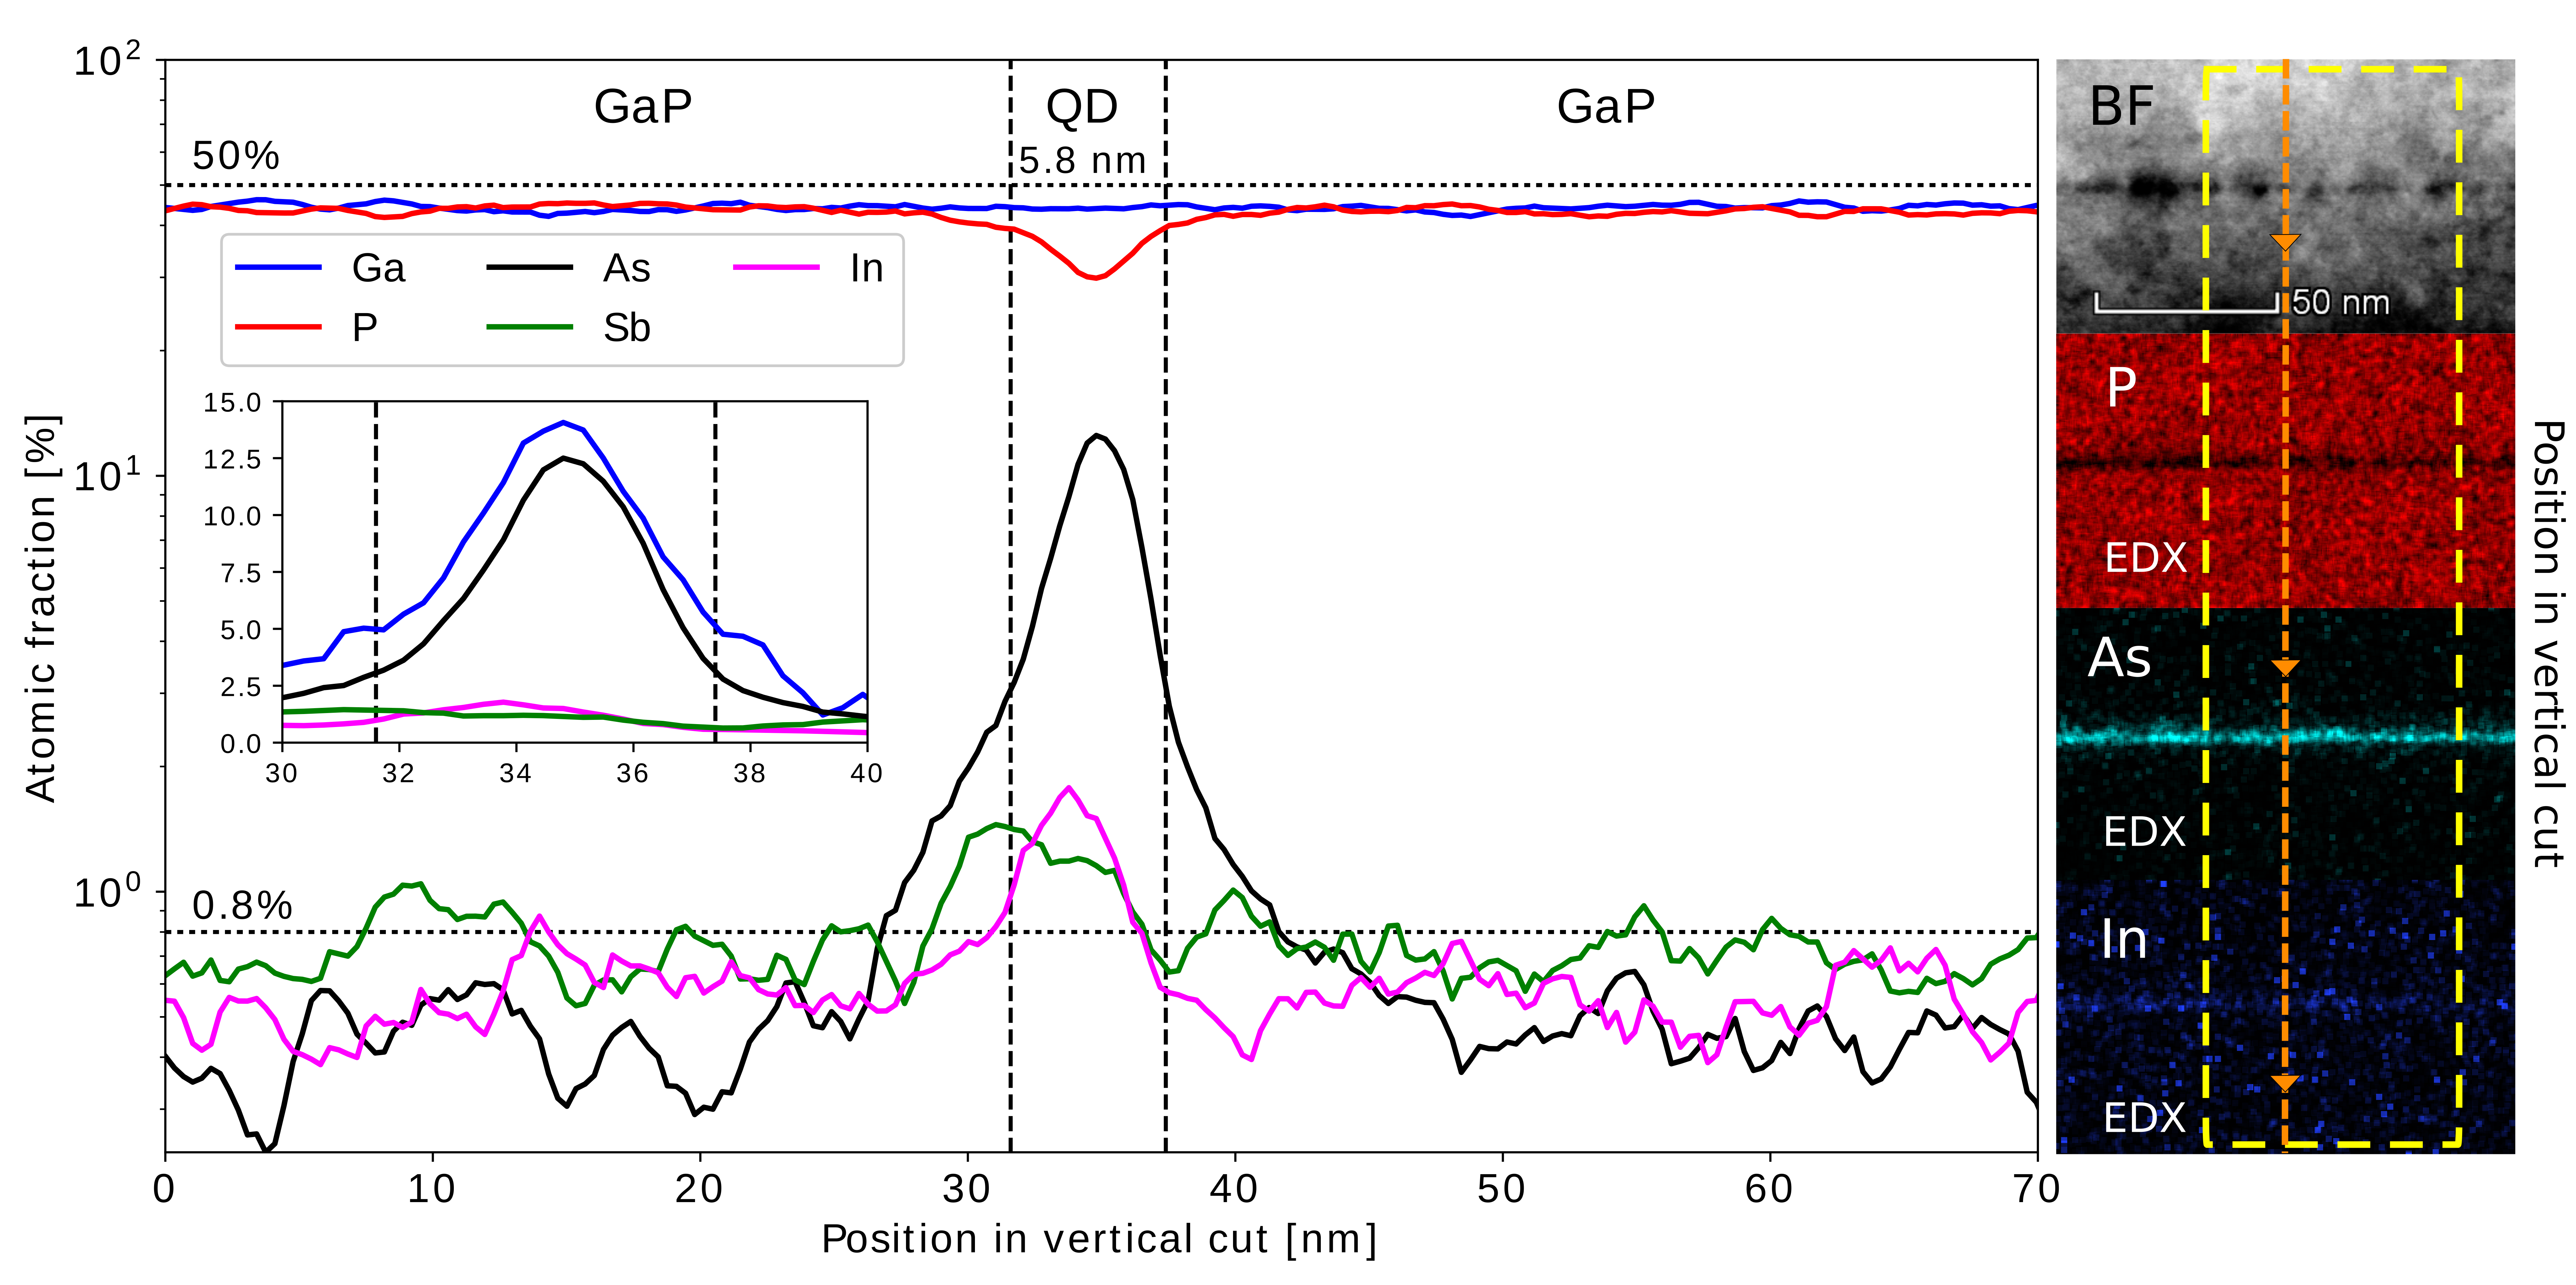
\includegraphics[width=1\linewidth]{/TEM/koncentrace_final_mapa2_QDinset}
	\caption{The atomic fraction vs. position in the vertical cut for all elements present in sample S$_\mathrm{cap}$ measured by EDX detector along the orange line in the right panel and averaged in the area circumferenced by the yellow broken curve. In QD area, i.~e., between the vertical positions of 30 and 40~nm in the cut, a substantial increase of In, As, Sb (compounds only in QD structures) and decrease of P (P is out of the QD structures) are observed. The inset shows the composition solely in the QD region. The column on right-hand side represents from top to bottom: cross-section TEM image of S$_\mathrm{cap}$ taken under strong-beam bright field condition using the (200) reflection perpendicular to the growth direction; and three EDX images measured at the same time as TEM measurements -- red one for P, white in As and purple in In.}
	\label{fig:TEM}
\end{figure}

We use the EDX data to estimate the concentration of individual elements in quaternary QD structure. Assuming that all phosphorus is bound in GaP, the concentration of Ga can be deconvoluted into Ga concentration in GaP $C_\mathrm{GaP}$ and in QD area $C_\mathrm{Ga}^\mathrm{QD}$ as
%
\begin{eqnarray}
C_\mathrm{Ga}=C_\mathrm{GaP}+C_\mathrm{Ga}^\mathrm{QD}=C_\mathrm{P}+C_\mathrm{Ga}^\mathrm{QD},
\end{eqnarray}
%
where $C_\mathrm{i}$ for $i \in \{\mathrm{Ga}, \mathrm{P}\}$ is the measured concentration of Ga and P. We assume the composition of our QDs in the form of In$_{1-x}$Ga$_{x}$As$_y$Sb$_{1-y}$, thus, we can calculate effective concetration in QD area as
%
\begin{eqnarray}
x=\frac{C_\mathrm{Ga}^\mathrm{QD}}{C_\mathrm{Ga}^\mathrm{QD}+C_\mathrm{In}^\mathrm{QD}},\qquad
y=\frac{C_\mathrm{As}^\mathrm{QD}}{C_\mathrm{As}^\mathrm{QD}+C_\mathrm{Sb}^\mathrm{QD}}.
\end{eqnarray}
%
Given the assumption that In, Ga and Sb are only in QD area, we can replace the concentration in this region with directly measured concentration by EDX. Finally, we give the estimation of $x$ and $y$ which we use in 8-band $\mathbf{k\cdot p}$ calculations of $x=84-93.5~\%$ and $y=68-91.5~\%$, see Fig.~\ref{fig:concentration_estimation}.


\begin{figure}
	\centering
	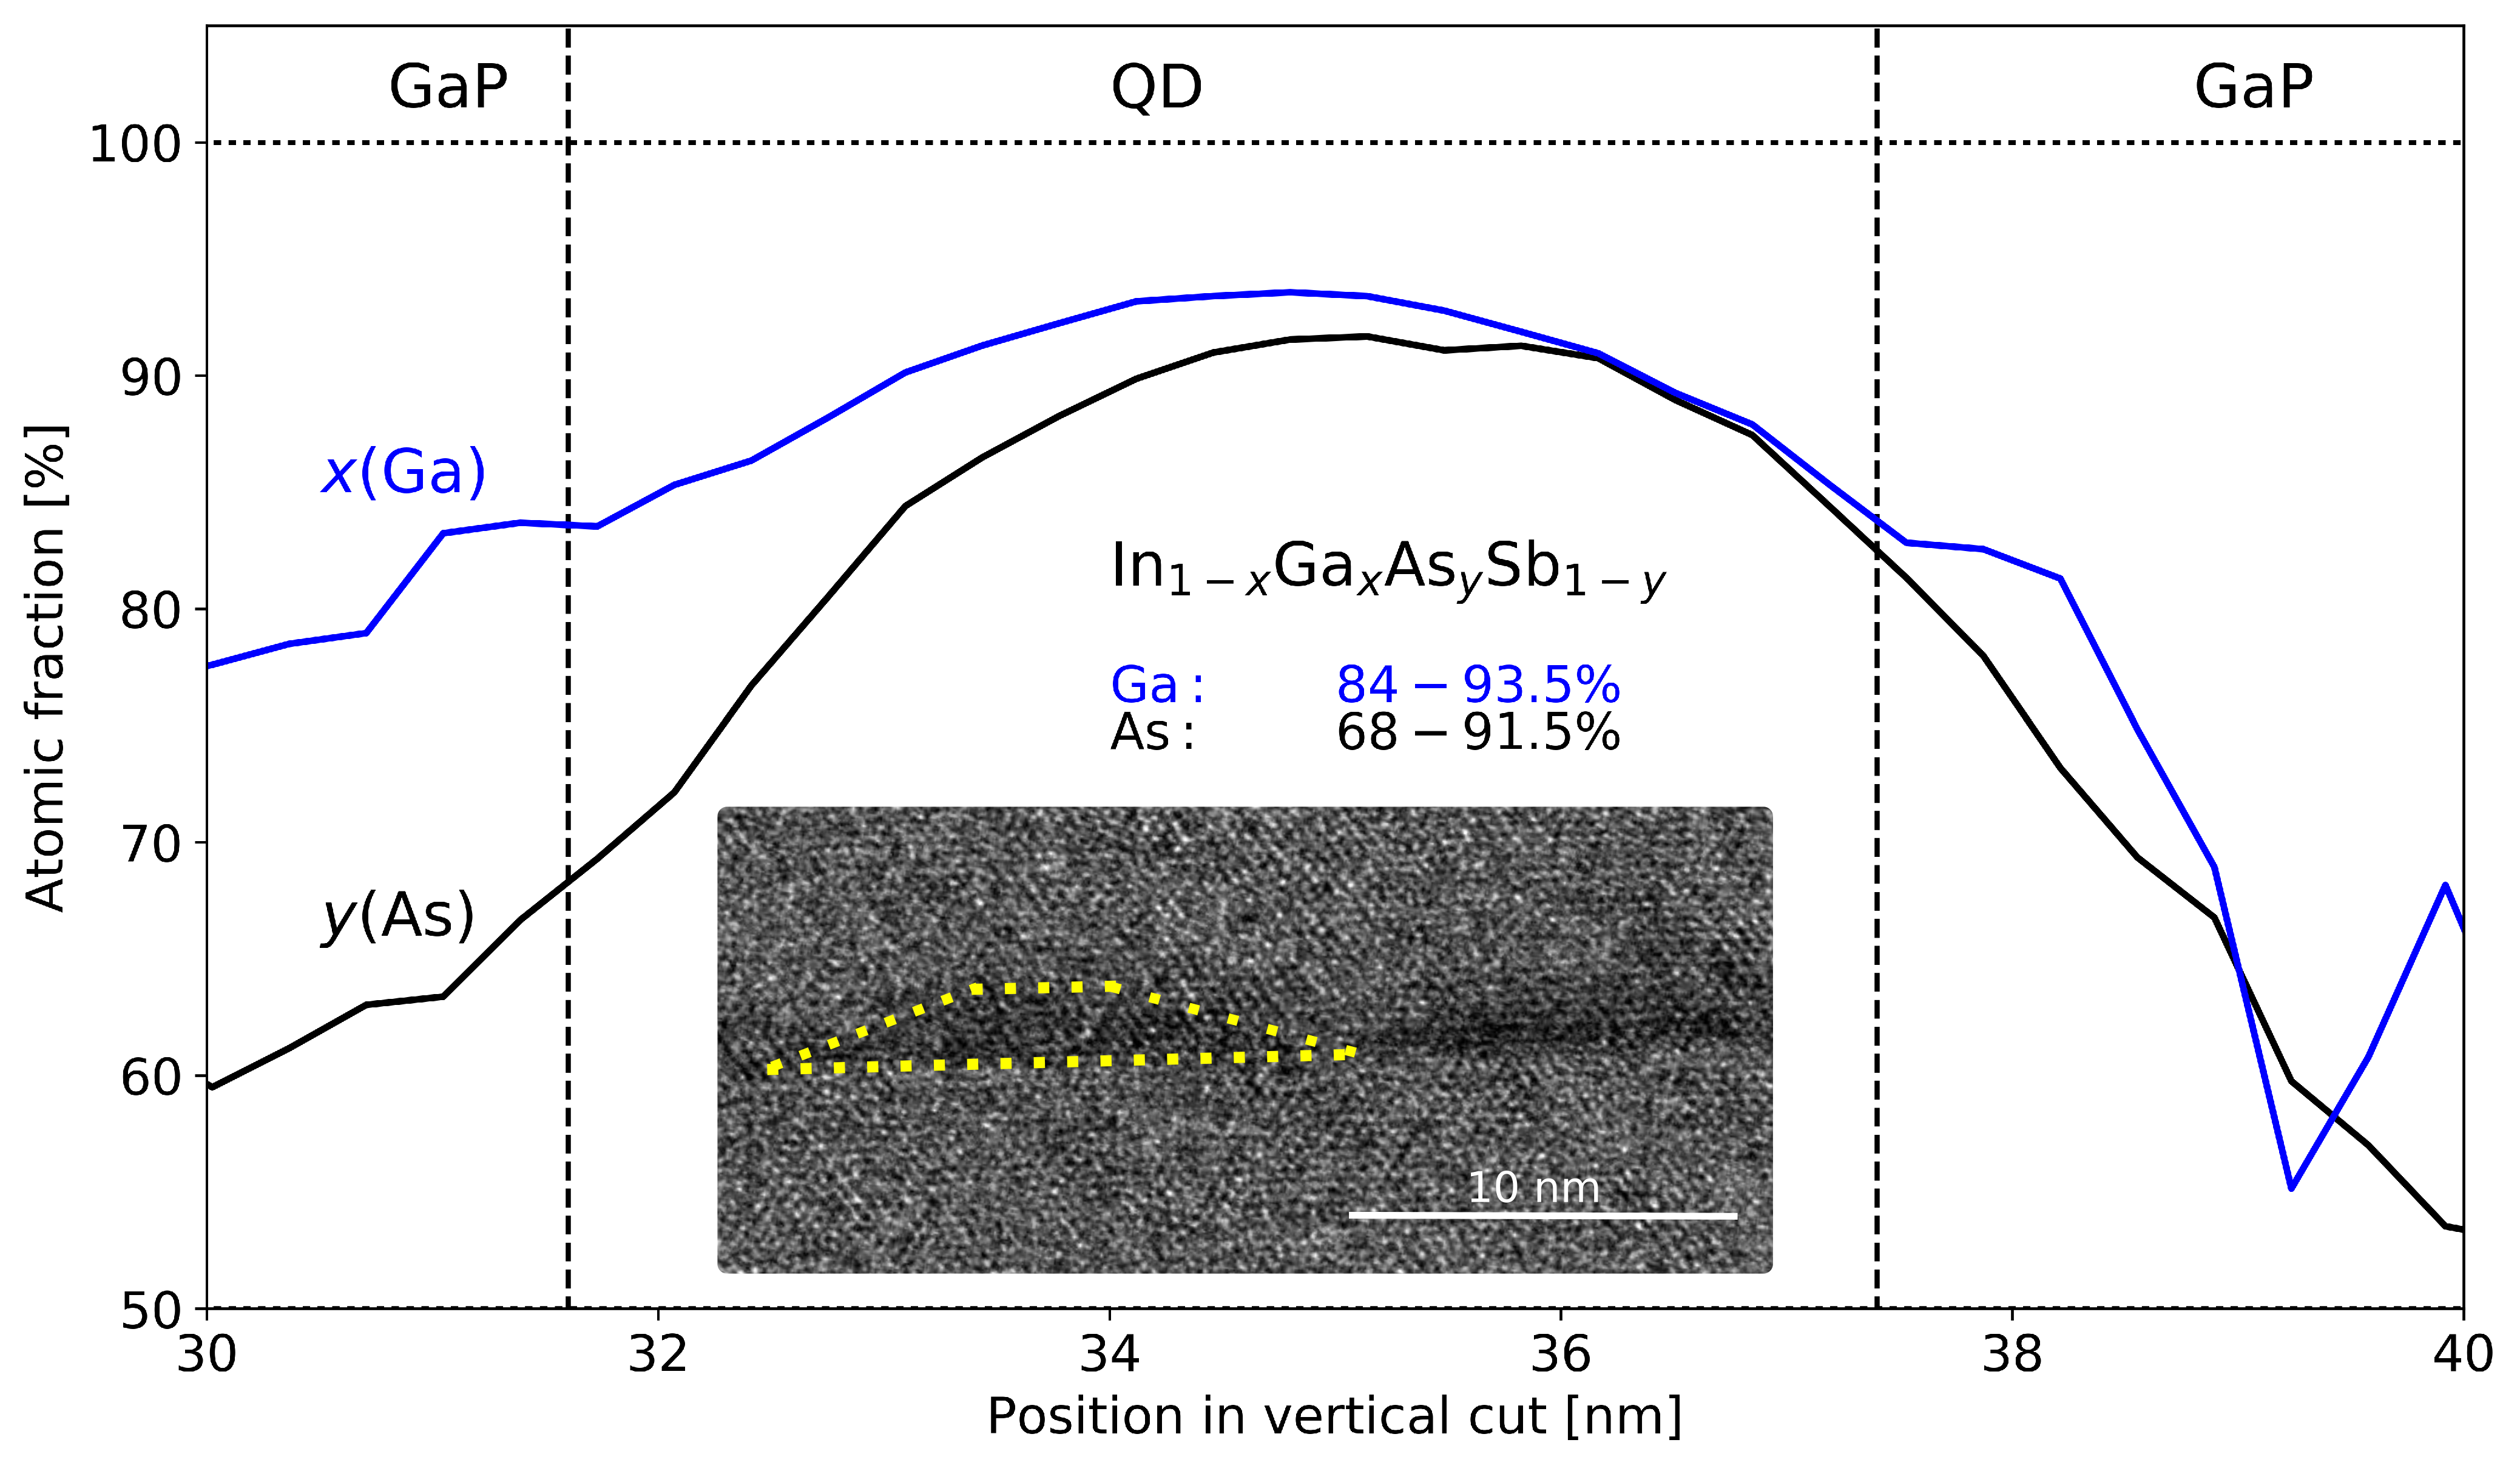
\includegraphics[width=0.85\linewidth]{/TEM/koncentrace_pro_nn} %rez_QD_konc_xy_bez}
	\caption{The estimated composition of QD area for sample S$_\mathrm{cap}$. We assume Ga and As concentration to be in the ranges of 84-93.5~\% and 68-91.5~\%, respectively. In inset we show the HRTEM image of a truncated-pyramid QD.}
	\label{fig:concentration_estimation}
\end{figure}

\clearpage

\section{Estimation of hydrostatic strain in GaAs layer}
For estimation of a hydrostatic component of the strain was performed room temperature Raman measurements of our samples. These measurements were obtained using NT-MDT spectrometer with a 100$\times$/0.7~NA long working length objective and the 532~nm laser. The scattered light was dispersed using a 1800~groove/mm grating and detected by a thermoelectrically cooled Si CCD camera. The spectra were recorded in $z(xy)z$ backscattering geometry.

Measured signals were fitted by the sum of 3 Lorentzian curves.
Let we focus to Raman signal around 290~cm$^{-1}$ where the TO phonon of strained GaAs QWs for our QDs samples is expected. Fig.~\ref{fig:raman} reports about $\sim$19~cm$^{-1}$ shift of TO phonon for our QDs samples compared to bulk material. Using a model~\cite{Montazeri_Nano2010}, we can use the shift to estimate the value of hydrostatic strain $\epsilon_{xx}$ 
\begin{equation}
k_\mathrm{TO}^2 = k_\mathrm{TO,B}^2 + (p+2q)\epsilon_{xx},
\end{equation}
where $k_\mathrm{TO}$ and $k_\mathrm{TO,B}$ are the Raman shifts of TO GaAs mode of strained and bulk GaAs, and $p$ and $q$ are phonon deformation potentials taken from Ref.~\cite{Cerdeira_PRB1972}.

The measured shifts of TO mode of $S_\mathrm{w/o}$ correspond to $\epsilon_{xx}=-0.032$, of $S_\mathrm{with}$ to $\epsilon_{xx}=-0.026$,  and for $S_\mathrm{cap}$ is $\epsilon_{xx}=-0.030$, which is in good agreement with the predicted hydrostatic strain component $\epsilon_{xx}=-0.034$ by the $\mathbf{k \cdot p}$ calculations, see Fig.~\ref{fig:raman_theory_wo}. %approximately three times less than predicted hydrostatic strain component by the $\mathbf{k \cdot p}$ calculations, see Fig.~\ref{fig:raman_theory_wo}.
\begin{figure}
	\centering
	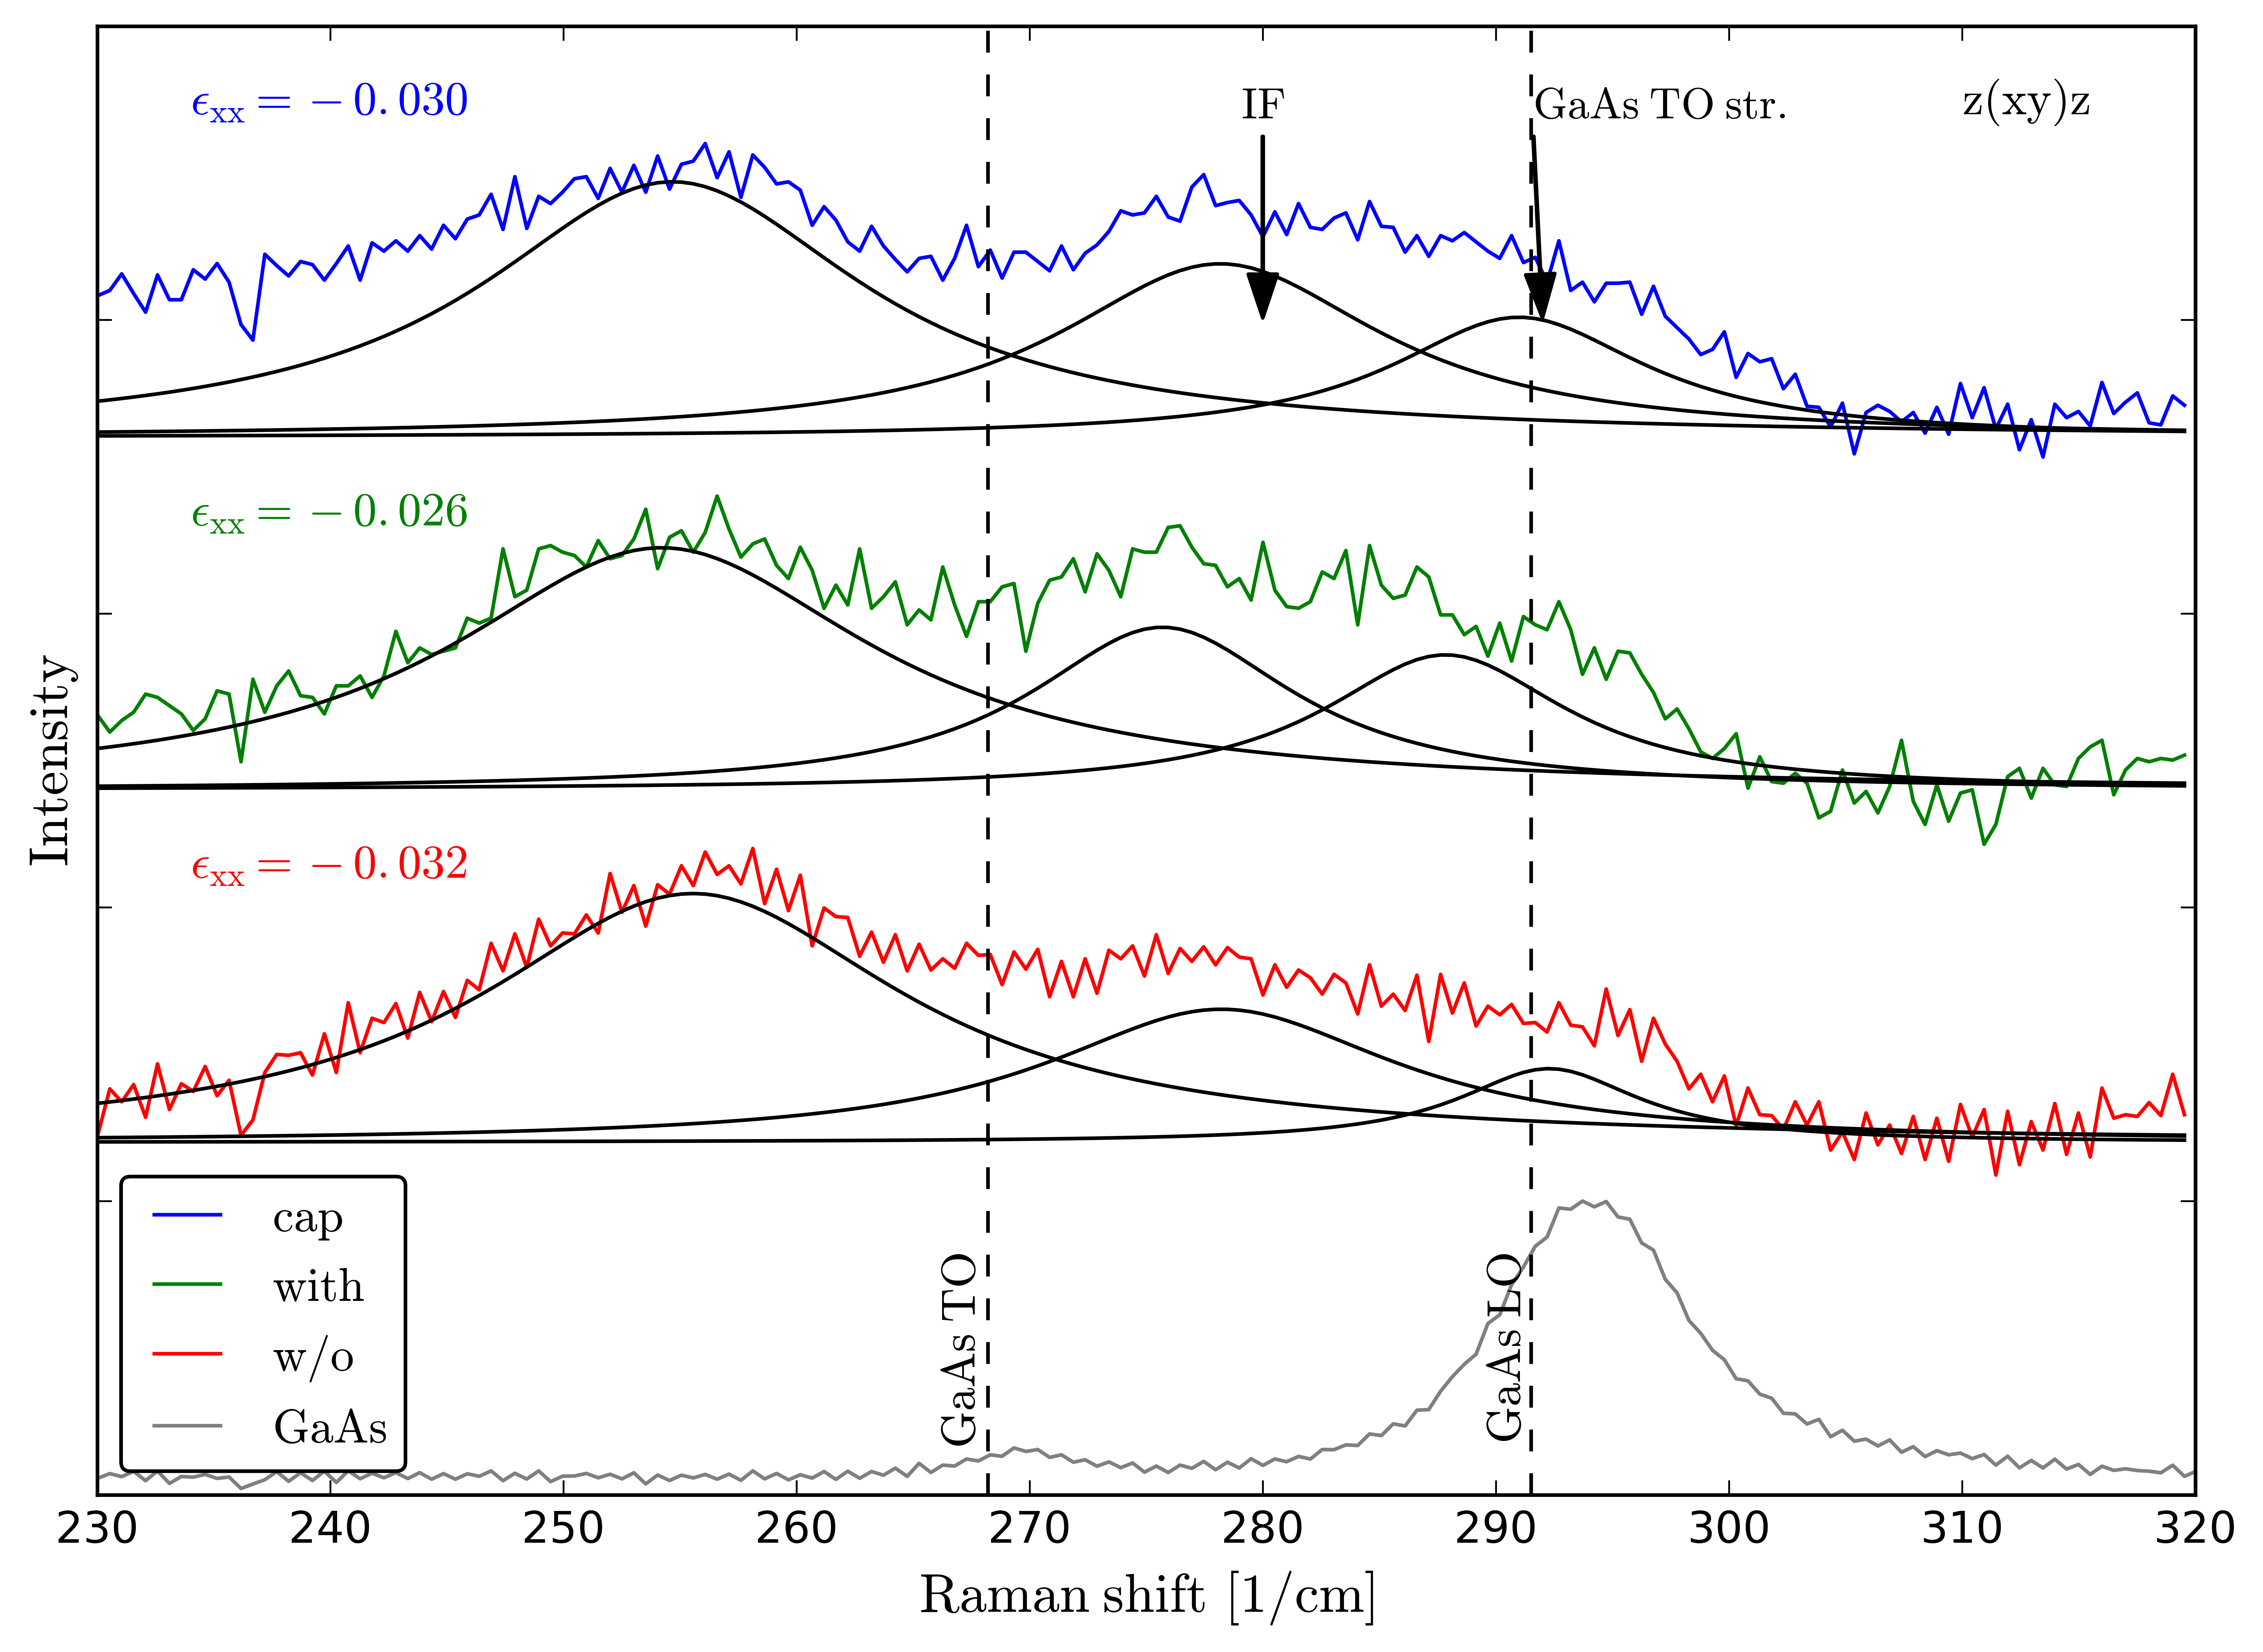
\includegraphics[width=0.85\linewidth]{/raman/Raman_TUB_and_GaAs_enlg_230_to_320_fit}
	\caption{Raman spectra of samples w/o QDs $S_\mathrm{w/o}$ (red), with QDs $S_\mathrm{with}$ (green) and capped QDs $S_\mathrm{cap}$ and bulk GaAs (grey). The dashed lines show reference GaAs TO and LO modes~\citep{Esther_Nanotech2013}. Calculated hydrostatic strain components $\epsilon_{xx}$ are presented in inset of the figure. A label IF corresponds to interface Raman band.}
	\label{fig:raman}
\end{figure}

\begin{figure}
	\centering
	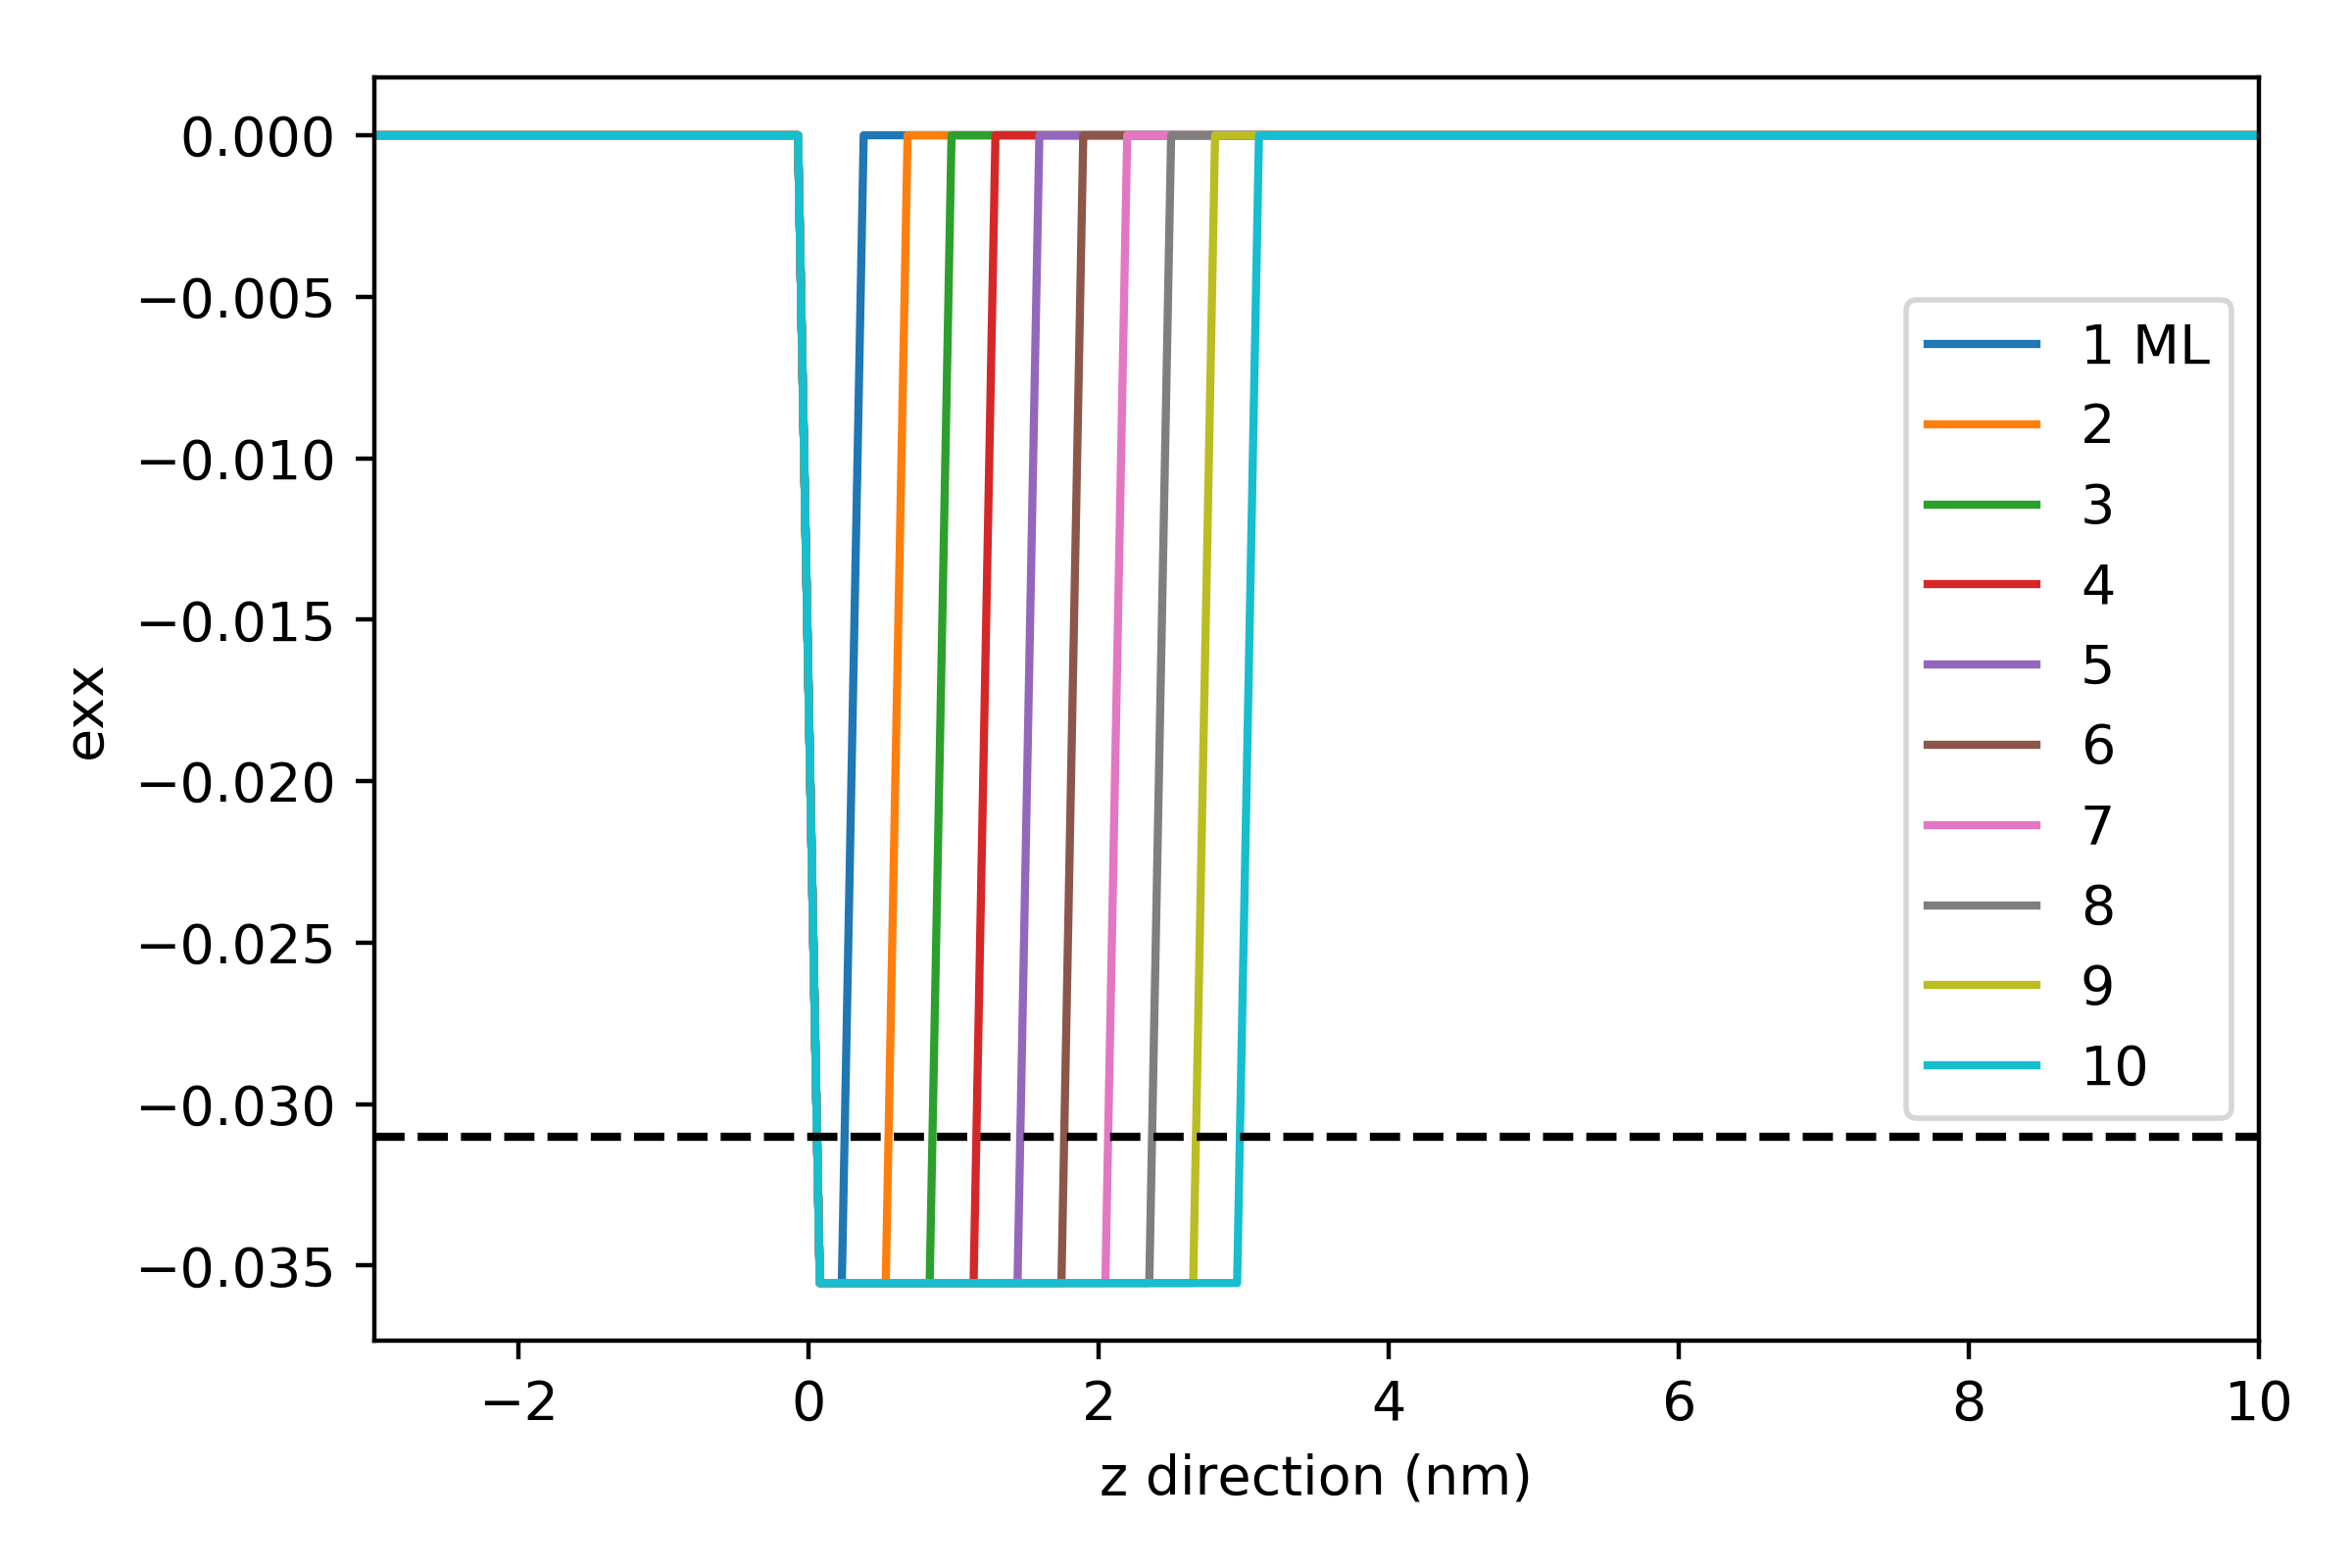
\includegraphics[width=0.85\linewidth]{/raman/eyy_vs_ML}
	\caption{Hydrostatic strain $\epsilon_{xx}$ calculated as a function of GaAs layer thickness in the sample $S_\mathrm{w/o}$. The experimental value is represented by a dashed curve. The calculations were made by the supervisor.}
	\label{fig:raman_theory_wo}
\end{figure}


\clearpage
\section{Experimental setup for photoluminescence measurements}
The PL measurements were performed using standard PL setup. The samples were positioned in the cryostat, cooled to 15~K and pumped by a laser diode with the wavelength of 405~nm with 0.05~mm$^2$ large spot size. The emitted emission signal was dispersed by a 1200~grooves/mm ruled grating designed to the wavelength of 750~nm and synchronously detected by a Si-avalanche photodiode (APD). We have performed the following PL experiments: (i) in intensity dependent measurements the laser power was varied by a neutral density (ND) filter over more than 4 orders of magnitude, (ii) in the temperature resolved PL temperature was changed from 15~K to room temperature, but for our samples and given integration time (0.3~s per one wavelength) we have not detected any PL signal at 300~K, (iii) the polarization of the PL was analyzed by a rotating achromatic half-wave retarder followed by a fixed linear polarizer.

In time-resolved experiments we have used laser with wavelength of 405~nm focused on 0.06~mm$^2$ area with pulse-width of 60~ps; emitted PL spectrum was dispersed again by 1200~grooves/mm ruled grating and detected by a Si-APD. We have performed the following TRPL experiments: (i) intensity resolved TRPL was measured at 15~K in 200~ns temporal window with resolution around 800~ps; the pumping power density was tuned by a ND filter in a range of 0.1--0.7~W/cm$^2$. The repetition rate of the laser was 5~MHz. (ii) In temperature resolved TRPL a temperature was changed on a range 15--150~K, the temporal window was modified to maximize the resolution from 200~ns for lower temperature to 25~ns for higher temperature. Tuning the temporal window is connected with changes in repetition rate, which was varied between 5 (for the temporal window 200~ns) and 80~MHz (for 25~ns).

Both experimental setups are schematically depicted in~Fig.~\ref{fig:Madrid_setup}.
\begin{figure}
	\centering
	\includegraphics[width=1\linewidth]{/PL/setup}
	\caption{Schematic of the (a) PL and (b) TRPL measurement setup. The picture of the TRPL setup is motivated by Ref.~\citep{TRPL_setup}.}
	\label{fig:Madrid_setup}
\end{figure}


\newpage
\section{Photoluminescence measurements}

The homogeneity of samples was tested by performing PL measurements on different areas of them. The results of those for different samples spots (distinguished by the type of the curve) and samples (different color) are depicted in the Fig.~\ref{fig:PL_homogenity}. We can see that samples are rather spatially homogeneous, hence our measurements might be considered as reproducible on the samples. %it is not necessary measured PL and TRPL in the same time. 

Let look at the emission structures around 1.8~eV. Firstly, we compare substrate emission in this spectral range with signal from our samples. We clearly see a broader band which is around 70~times smaller than emission from our samples so that we neglect this band. For $S_\mathrm{w/o}$ are shown PL with two maxima located at 1.83 and 1.86~eV, respectively. The PL signal of samples with QDs are shifted to smaller energies: the maxima are located at 1.78~eV for $S_\mathrm{with}$ and 1.74~eV for $S_\mathrm{cap}$. Finally, let us notice that the PL from $S_\mathrm{with}$ is twice stronger compared to other samples.
\begin{figure}
	\centering
	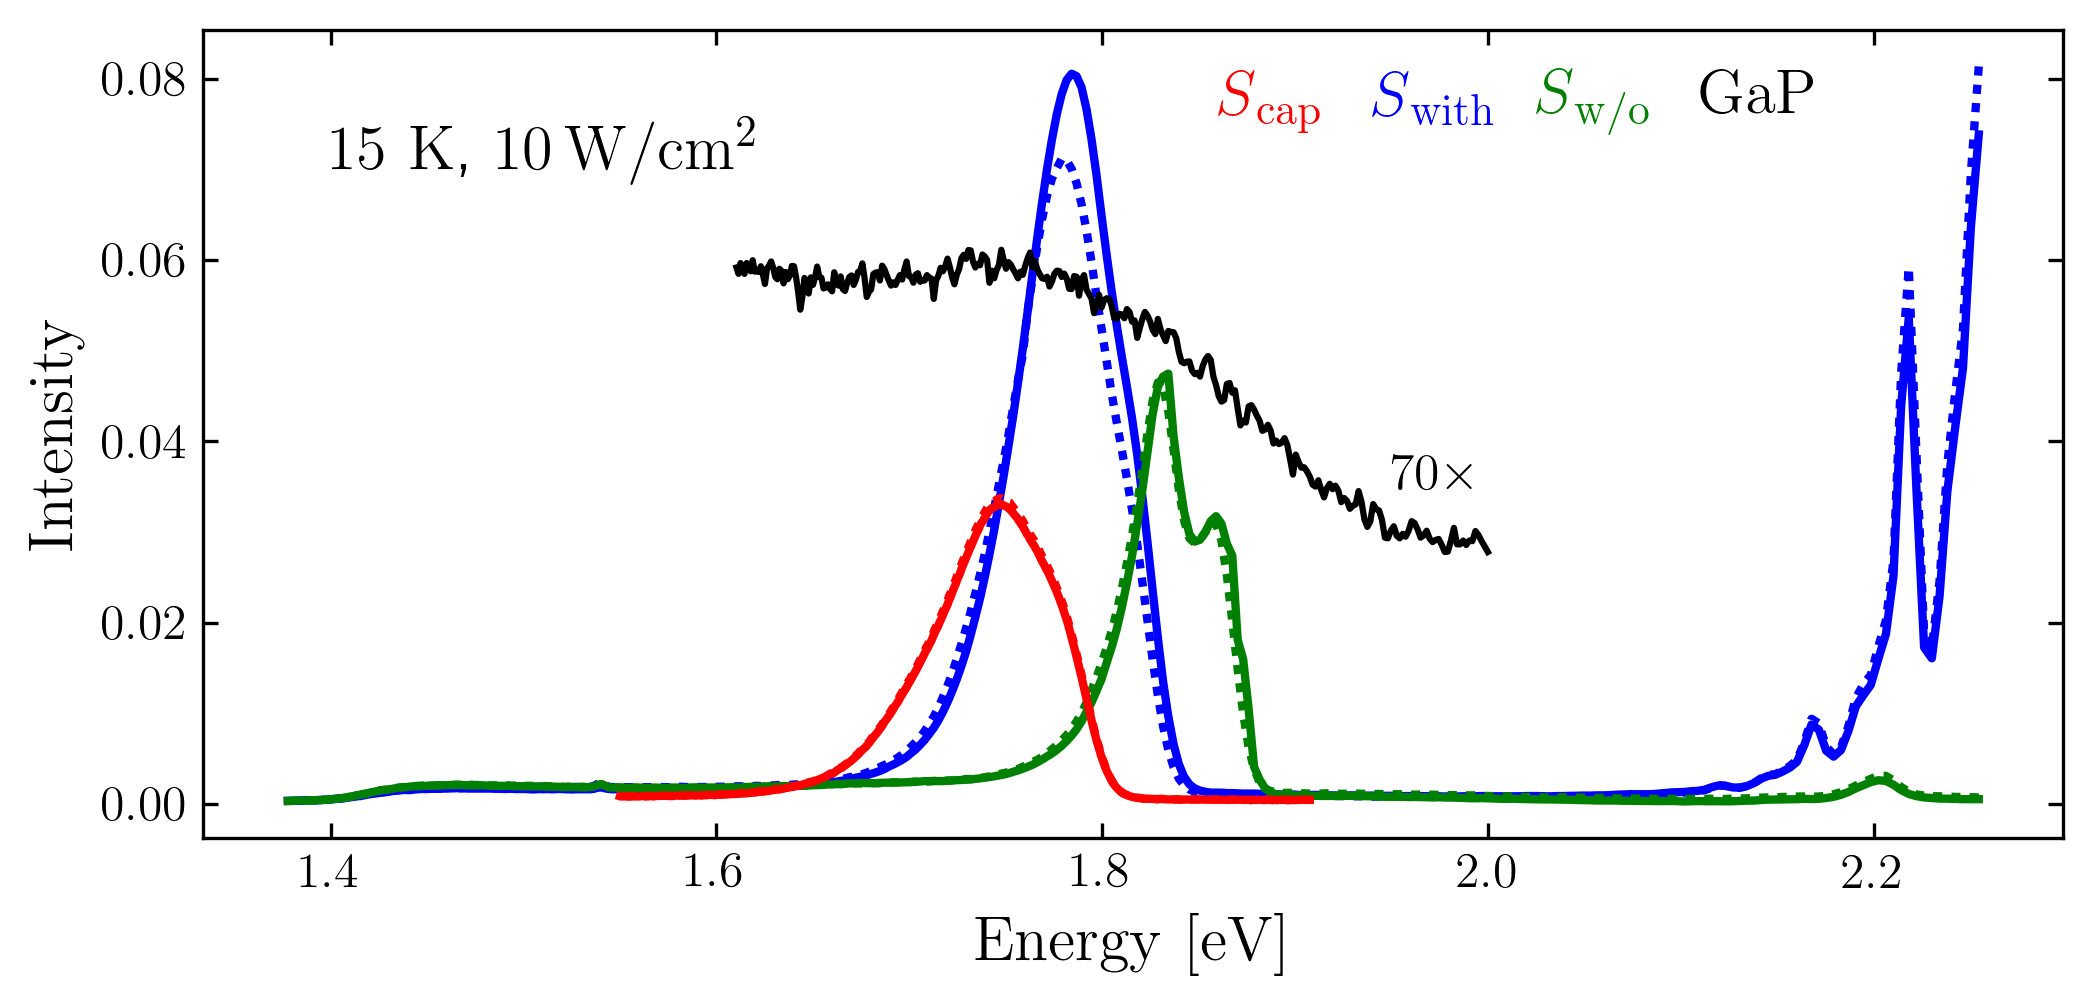
\includegraphics[width=1\linewidth]{/PL/all__IntensityVSen_GaP}
	\caption{PL for samples $S_\mathrm{w/o}$ (green lines), $S_\mathrm{with}$ (blue) and $S_\mathrm{cap}$ (red) measured at 15~K and 10~W/cm$^2$ on several places on samples (different curve types). PL from our samples is compared with emission from GaP substrate (black).}
	\label{fig:PL_homogenity}
\end{figure}

\subsection{Excitation intensity dependent PL}
\label{sec:intensity_PL_TU}
PL for each sample and excitation density $D$ was fitted by sum of three Gaussian curves and the individual bands corresponding to different optical transitions was studied. 

\subsubsection*{Sample without QDs $\mathbf{S_\mathrm{w/o}}$}
\label{Sec:PL_int_wo}
\begin{figure}
	\centering
	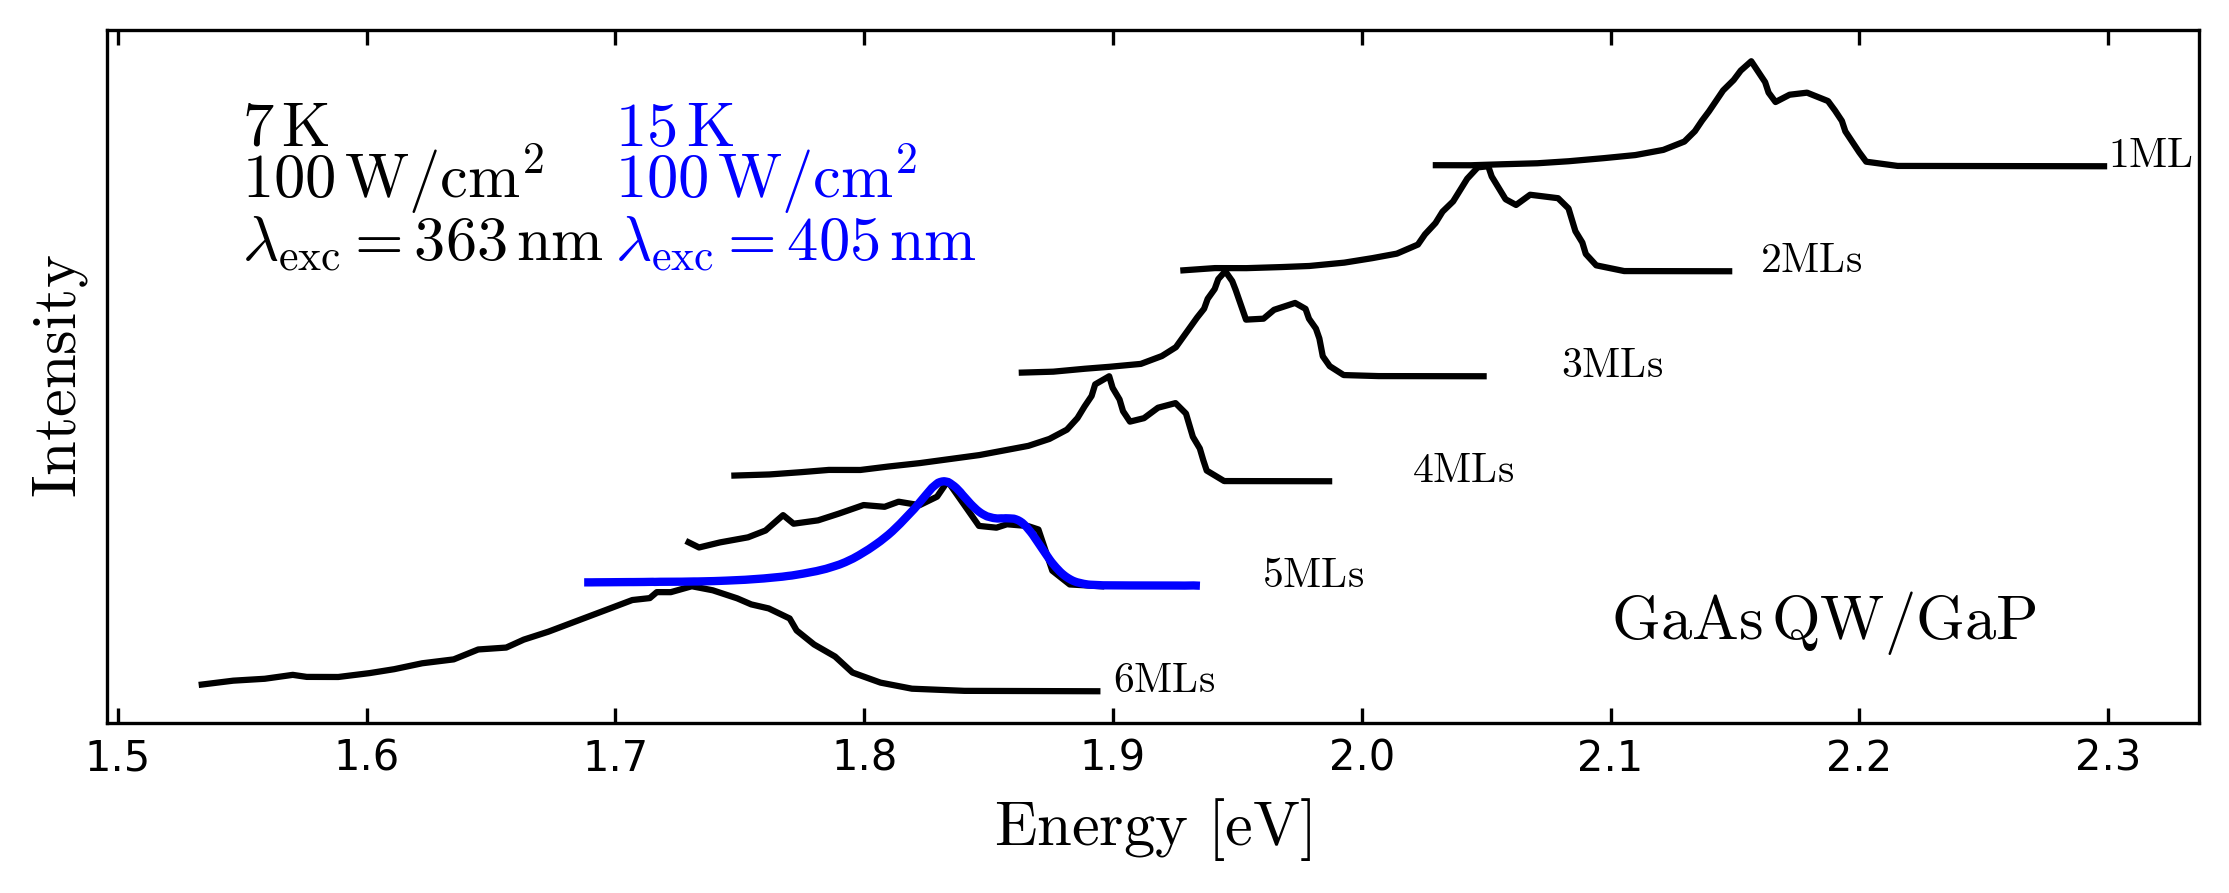
\includegraphics[width=0.9\linewidth]{/PL/12027_ref_GaAs_5ML_new}
	\caption{The comparison of the spectrum of $S_\mathrm{w/o}$ (blue) with set of samples with variable thickness taken from~Ref.~\citep{Prieto_APL1997} (black). The measurement temperature of 15~K (7~K), excitation wavelength of 405~nm (363~nm) in our (in ref.~\citep{Prieto_APL1997}) were used. Excitation density in both experiments was 100~W/cm$^2$. We can see a good match of sample $S_\mathrm{w/o}$ with 5ML thick GaAs QW from Ref.~\citep{Prieto_APL1997}.}
	\label{fig:12027_ref}
\end{figure}


\begin{figure}
	\centering
	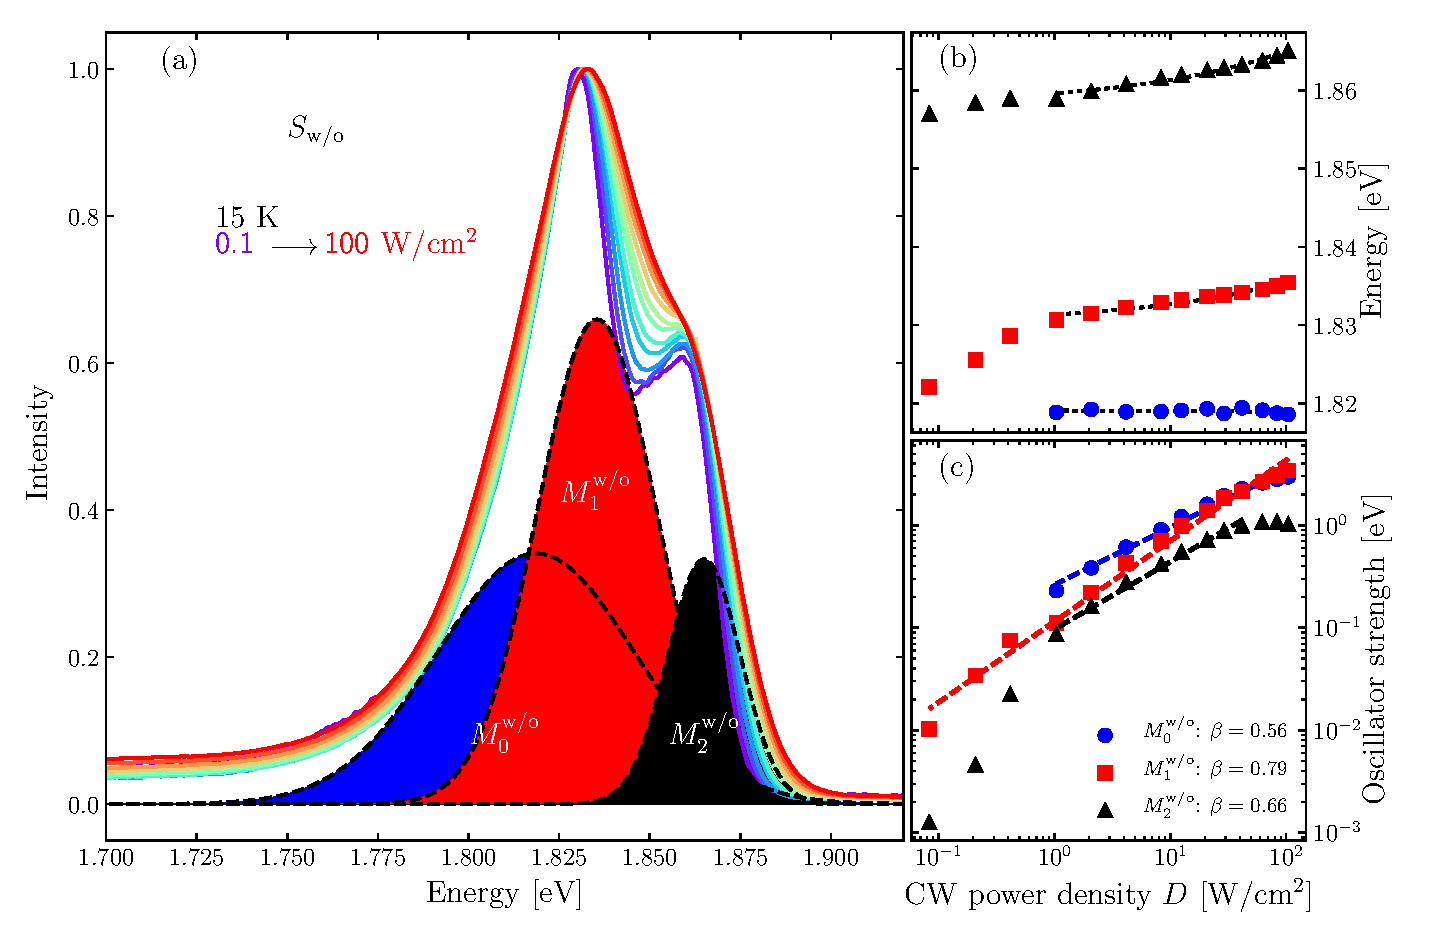
\includegraphics[width=0.9\linewidth]{/PL/intensity/12027_11011_norm_PL_int}
	\caption{(a) PL spectra of $S_\mathrm{w/o}$ measured for several excitation density in the range 0.1 and 100~W/cm$^2$. The fit by the sum of three Gaussian curves is shown for 100~W/cm$^2$ and the individual bands are presented by shaded area: $M_0^\mathrm{w/o}$ (blue), $M_1^\mathrm{w/o}$ (red) and $M_2^\mathrm{w/o}$ (black). In (b) we show power dependence of the energy of individual bands and their fits by Eq.~(\ref{eq:PL_intmodel}) (dotted curves). Panel (c) depicts the oscillators strength of the bands in log-log scale and their fits by linear lines (broken lines), respectively. The slopes of the linear fit $\beta$ (exponent in linear scale) are presented in the legend of panel (c). Individual transitions in panels (b) and (c) are represented by: $M_0^\mathrm{w/o}$ (blue circles), $M_1^\mathrm{w/o}$ (red squares) and $M_2^\mathrm{w/o}$ (black triangles).}
	\label{fig:QD_wo_int}
\end{figure}
Three emission bands of sample $S_\mathrm{w/o}$ labelled from smaller to greater localization energy $M_0^\mathrm{w/o}$, $M_1^\mathrm{w/o}$ and $M_2^\mathrm{w/o}$, respectively, are related to electrons in the $X_{xy}$ (the $X$ bands for GaAs strained to GaP are split into $X_z$ and $X_{xy}$ where $z$ indicates growth direction) GaAs minima recombination with heavy holes in the $\Gamma$ band in GaAs layer. Ref.~\citep{Prieto_APL1997} discusses the effect of GaAs layer thickness on emission spectra where they observed overally an energy shift, with the thickness of the layer, but the energy separations between corresponding bands stayed nearly independent of layer thickness. Similarly as in Ref.~\citep{Prieto_APL1997}, where those were 12 and 32~meV, we detect similar ones and depending on the excitation density we have found them to be between 12--17~meV and 40--46~meV. Hence, the peaks cannot be attributed to thickness fluctuations, but instead they can be connected with phonon-assisted transitions. The energies of the phonons closely correspond to TA and LA phonon energies in GaP~\citep{Prieto_APL1997}. In Fig.~\ref{fig:12027_ref} PL of $S_\mathrm{w/o}$ is compared with studied set taken from Ref.~\citep{Prieto_APL1997}.



In Fig.~\ref{fig:QD_wo_int}(a) we show PL spectra of the sample with increasing $D$ and their deconvolution into individual band by Gaussian fits. The energy-shift is visualized in Fig.~\ref{fig:QD_wo_int}(b), where PL peak energies as a function $D$ for individual bands are plotted and fitted with %usually used formula~\citep{Hatami_apl1995_intmodel,Glaser_apl1996_intmodel,Ledentsov_prb1995_intmodel} derived for spatially indirect optical transition in quantum wells (QWs) and QDs
%
formula allow us distinguish state filling and band bending effect~\cite{Abramkin_blueshift_analytical}
\begin{equation}
E(D)=E_\mathrm{I}+\left(U_\mathrm{e}+U_\mathrm{h}\right) \ln\left(D \right)+\gamma D^{1/3}, \label{eq:PL_intmodel}
\end{equation}
%
where $E_\mathrm{I}$ is extrapolation energy to $D=0$~W/cm$^2$, $U_\mathrm{e}$ ($U_\mathrm{h}$) is Urbach energy tail for electrons (holes) and $\gamma$ is bend bending parameter.% constant which describes the gradient of the energy-shift. 
%The energy evolutions of the bands are well characterized with~Eq.~(\ref{eq:PL_intmodel}). The bands $M_1^\mathrm{w/o}$ and $M_2^\mathrm{w/o}$ are slightly shifted to blue with increasing $D$, these blue-shifts are described by almost identical $\gamma$, whereas $M_0^\mathrm{w/o}$ is rather independent on $D$ or slightly red-shifted.

The energy evolutions of the bands are well characterized with~Eq.~(\ref{eq:PL_intmodel}). The bands $M_1^\mathrm{w/o}$ and $M_2^\mathrm{w/o}$ are slightly shifted to blue with increasing $D$, whereas $M_0^\mathrm{w/o}$ is rather independent on $D$ or slightly red-shifted. Based on the values of parameters in the model~(\ref{eq:PL_intmodel}) we determined the type of band alignment: (i) $M_0^\mathrm{w/o}$ and $M_1^\mathrm{w/o}$ are types-I without ($U_\mathrm{e}+U_\mathrm{h}$ is almost zero) or with blue-shift described only by Urbach energy tails ($U_\mathrm{e}+U_\mathrm{h}=1$~meV), (ii) whereas $M_2^\mathrm{w/o}$ has type-II band alignment with the same Urbach tails as $M_1^\mathrm{w/o}$ but for proper description of its blue-shift the parameter $\gamma$ is necessary ($\gamma=3\pm2$~meVW$^{-1/3}$cm$^{2/3}$).





The oscillator strengths in Fig.~\ref{fig:QD_wo_int}(c) of $M_0^\mathrm{w/o}$, $M_1^\mathrm{w/o}$ follow a linear dependence in log-log graph with the excitation power ($\propto D^\beta$) in the whole measured range, indicating that there is neither saturation of electronic states nor the activation of the non-radiative events. The emission of $M_2^\mathrm{w/o}$ is linear only in the power density range 1 and 30~W/cm$^2$, under the range PL is saturated.

%%%%%%%%%%%%%%%%%%%%%%%%%%%%%%%%%%%%%%%%%%%%%%%
\subsubsection*{Sample with QDs $\mathbf{S_\mathrm{with}}$}
\begin{figure}
	\centering
	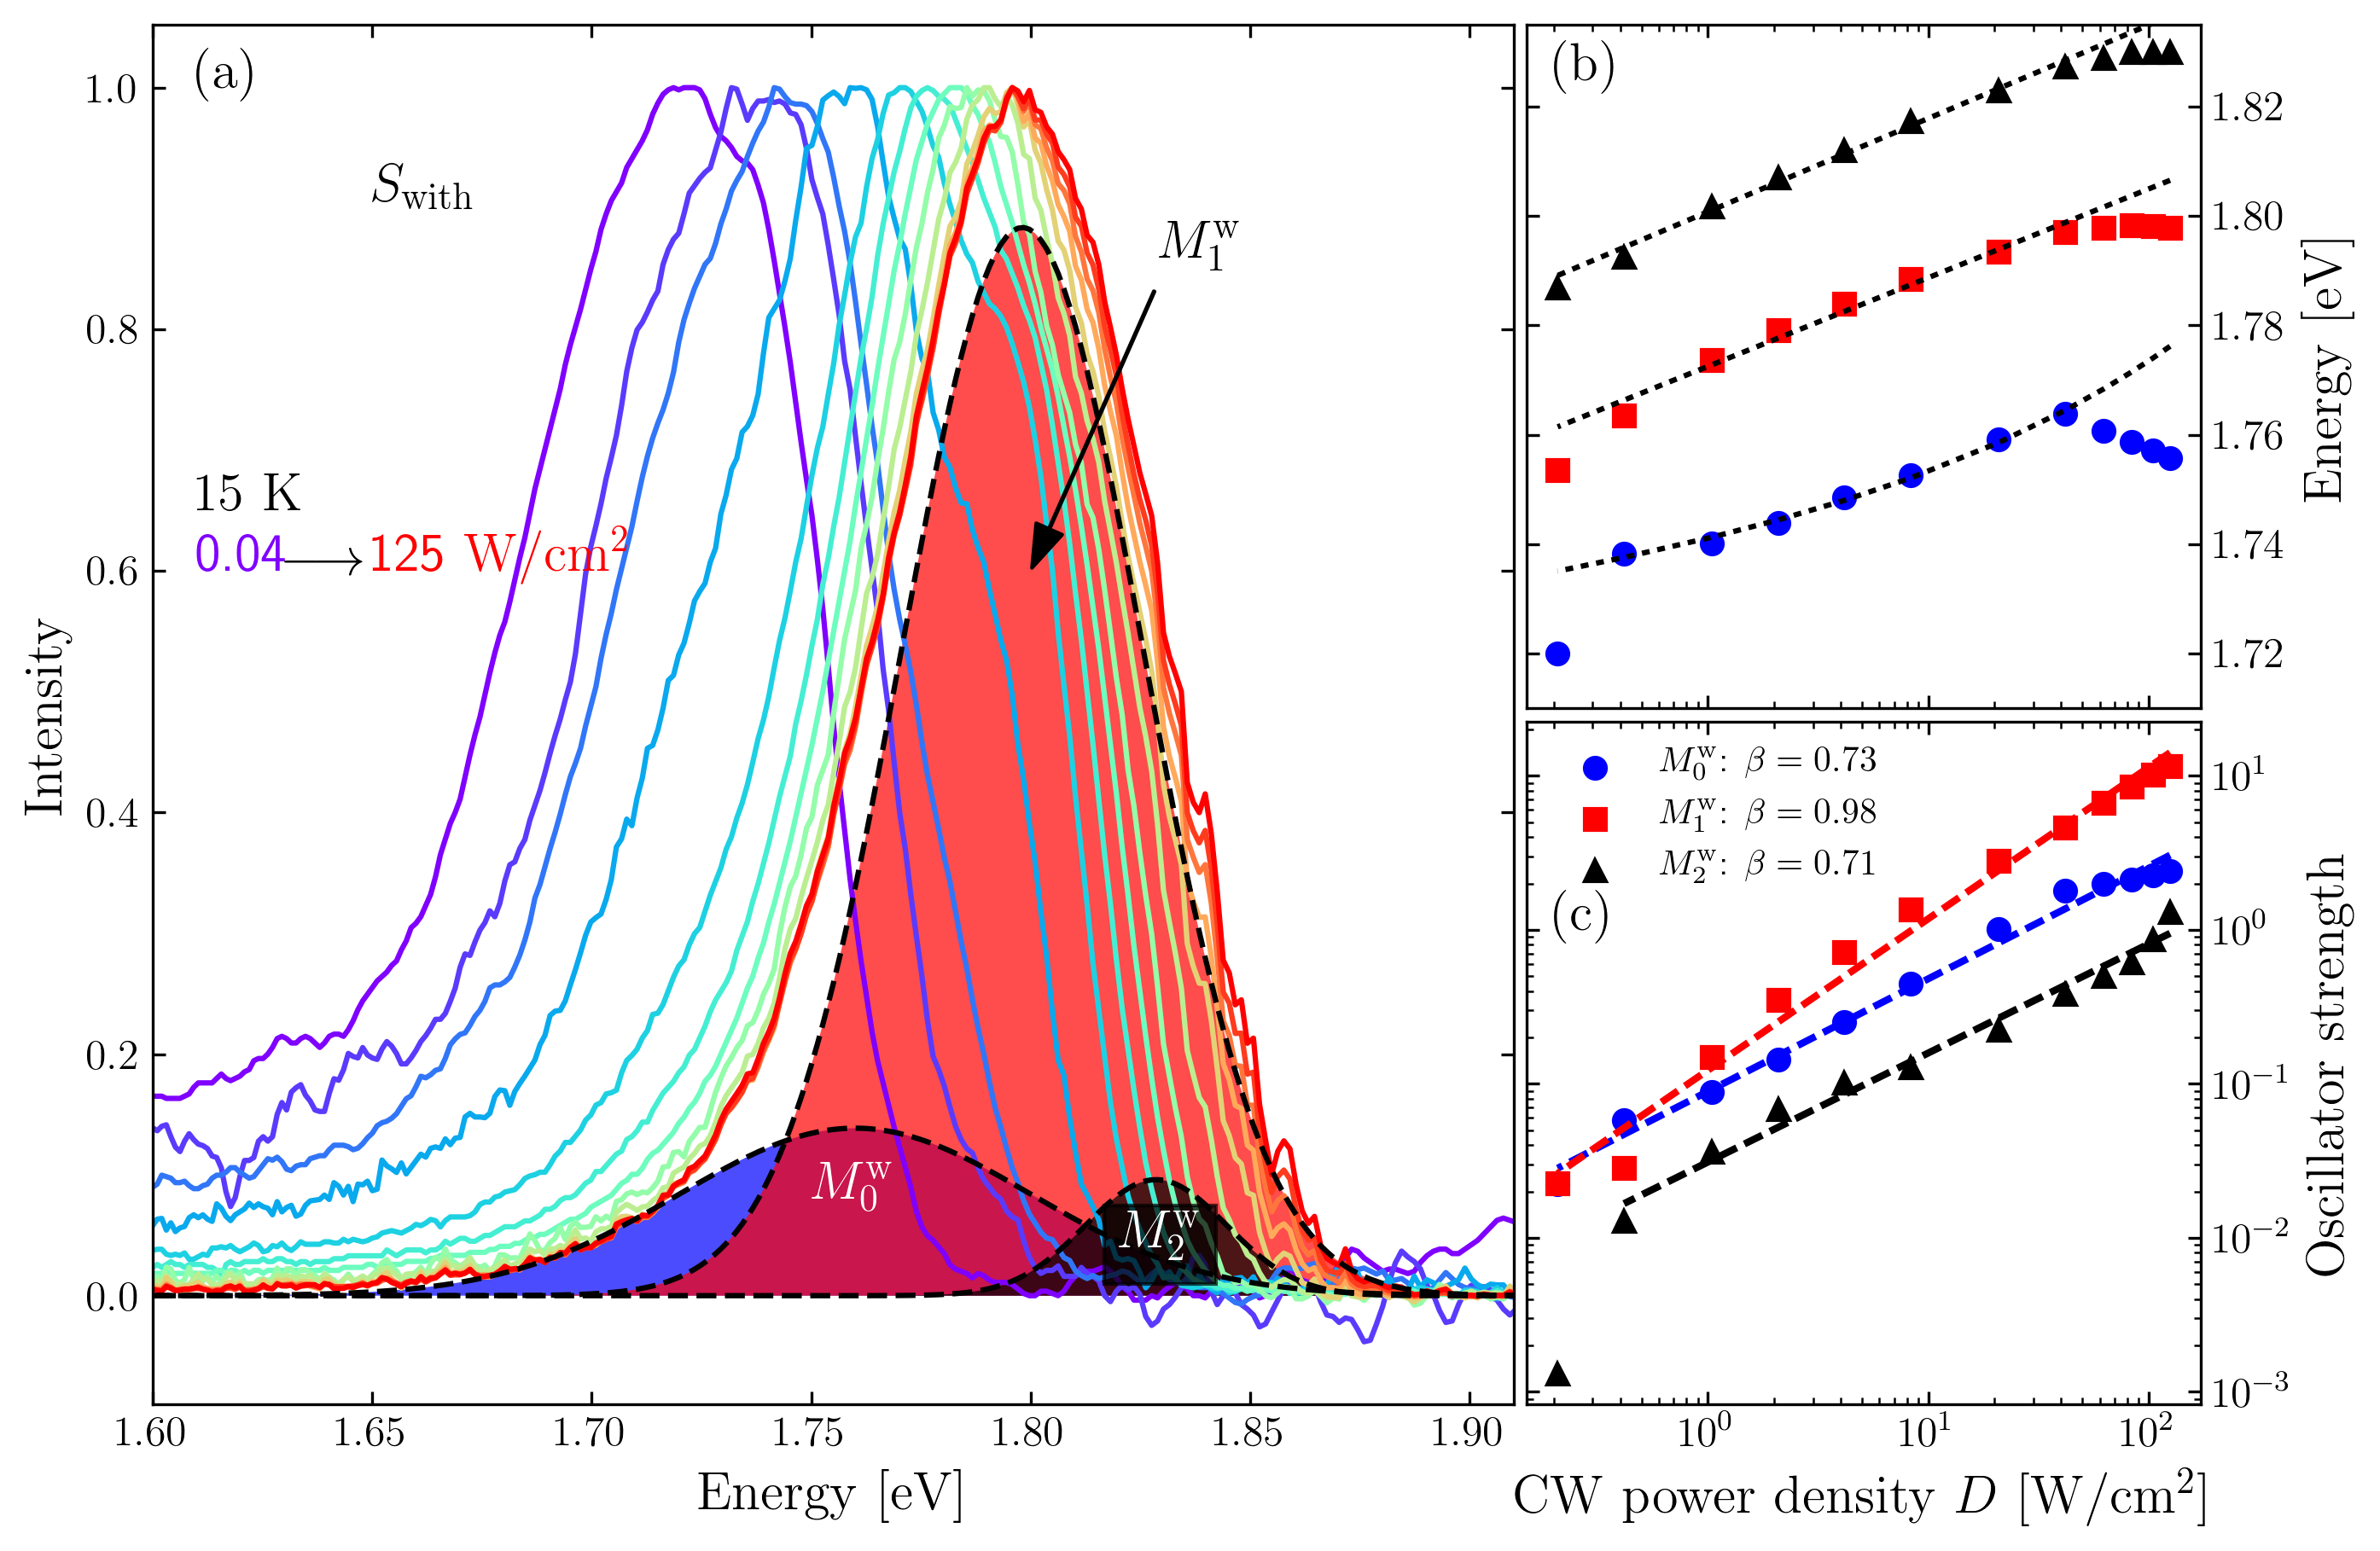
\includegraphics[width=0.9\linewidth]{/PL/intensity/12040_1113_norm_PL_int_typIvsII}
	\caption{(a) PL spectra of $S_\mathrm{with}$ as a function of excitation density were measured from 0.04 to 125~W/cm$^2$ and deconvolved by three Gaussian profiles ($M_0^\mathrm{w}$ blue, $M_1^\mathrm{w}$ red and $M_2^\mathrm{w}$ black shaded area). Fitted parameters - energy and oscillator strength are depicted in panels (b) and (c), respectively. Energies are fitted by Eg.~\ref{eq:PL_intmodel} (dotted curves in (b)), oscillator strengths by linear curve (dashed lines in (c)).}
	\label{fig:QD_w_int}
\end{figure}

Three Gaussian profiles ($M_0^\mathrm{w}$, $M_1^\mathrm{w}$ and $M_2^\mathrm{w}$) in PL spectra were fitted and studied as a function of excitation density $D$ in the range between 0.04 and 125~W/cm$^2$, see Fig.~\ref{fig:QD_w_int}. In Fig.~\ref{fig:QD_w_int}(b) and (c) we show the emission energy and oscillator strength of individual bands as a function of $D$, respectively. Analysing blue-shift of individual bands we distinguish type-II aligned $M_0^\mathrm{w}$ transition and type-I for $M_1^\mathrm{w}$ and $M_2^\mathrm{w}$. Interestingly, $M_1^\mathrm{w}$ and $M_2^\mathrm{w}$ are proportional to $\ln(D)$ via same constant ($U_\mathrm{e}+U_\mathrm{h}=7$~meV) which leads us to meaning that these transitions originated from the same structure. 
%The energies of $M_0^\mathrm{w}$ and $M_1^\mathrm{w}$ are fitted by Eq.~\ref{eq:PL_intmodel}, but we can see the third root behaviour only in the beginning of the dependence, then the energies start to be saturated. The whole evolution of energy versus pumping power is much better characterized using the self-consistent multi-particle calculations as in Ref.~\citep{Klenovsky2017}.

The dependencies for oscillator strengths were fairly well fitted by the linear function in the whole range.




\subsubsection*{Sample with capped QDs $\mathbf{S_\mathrm{cap}}$}
\begin{figure}
	\centering
	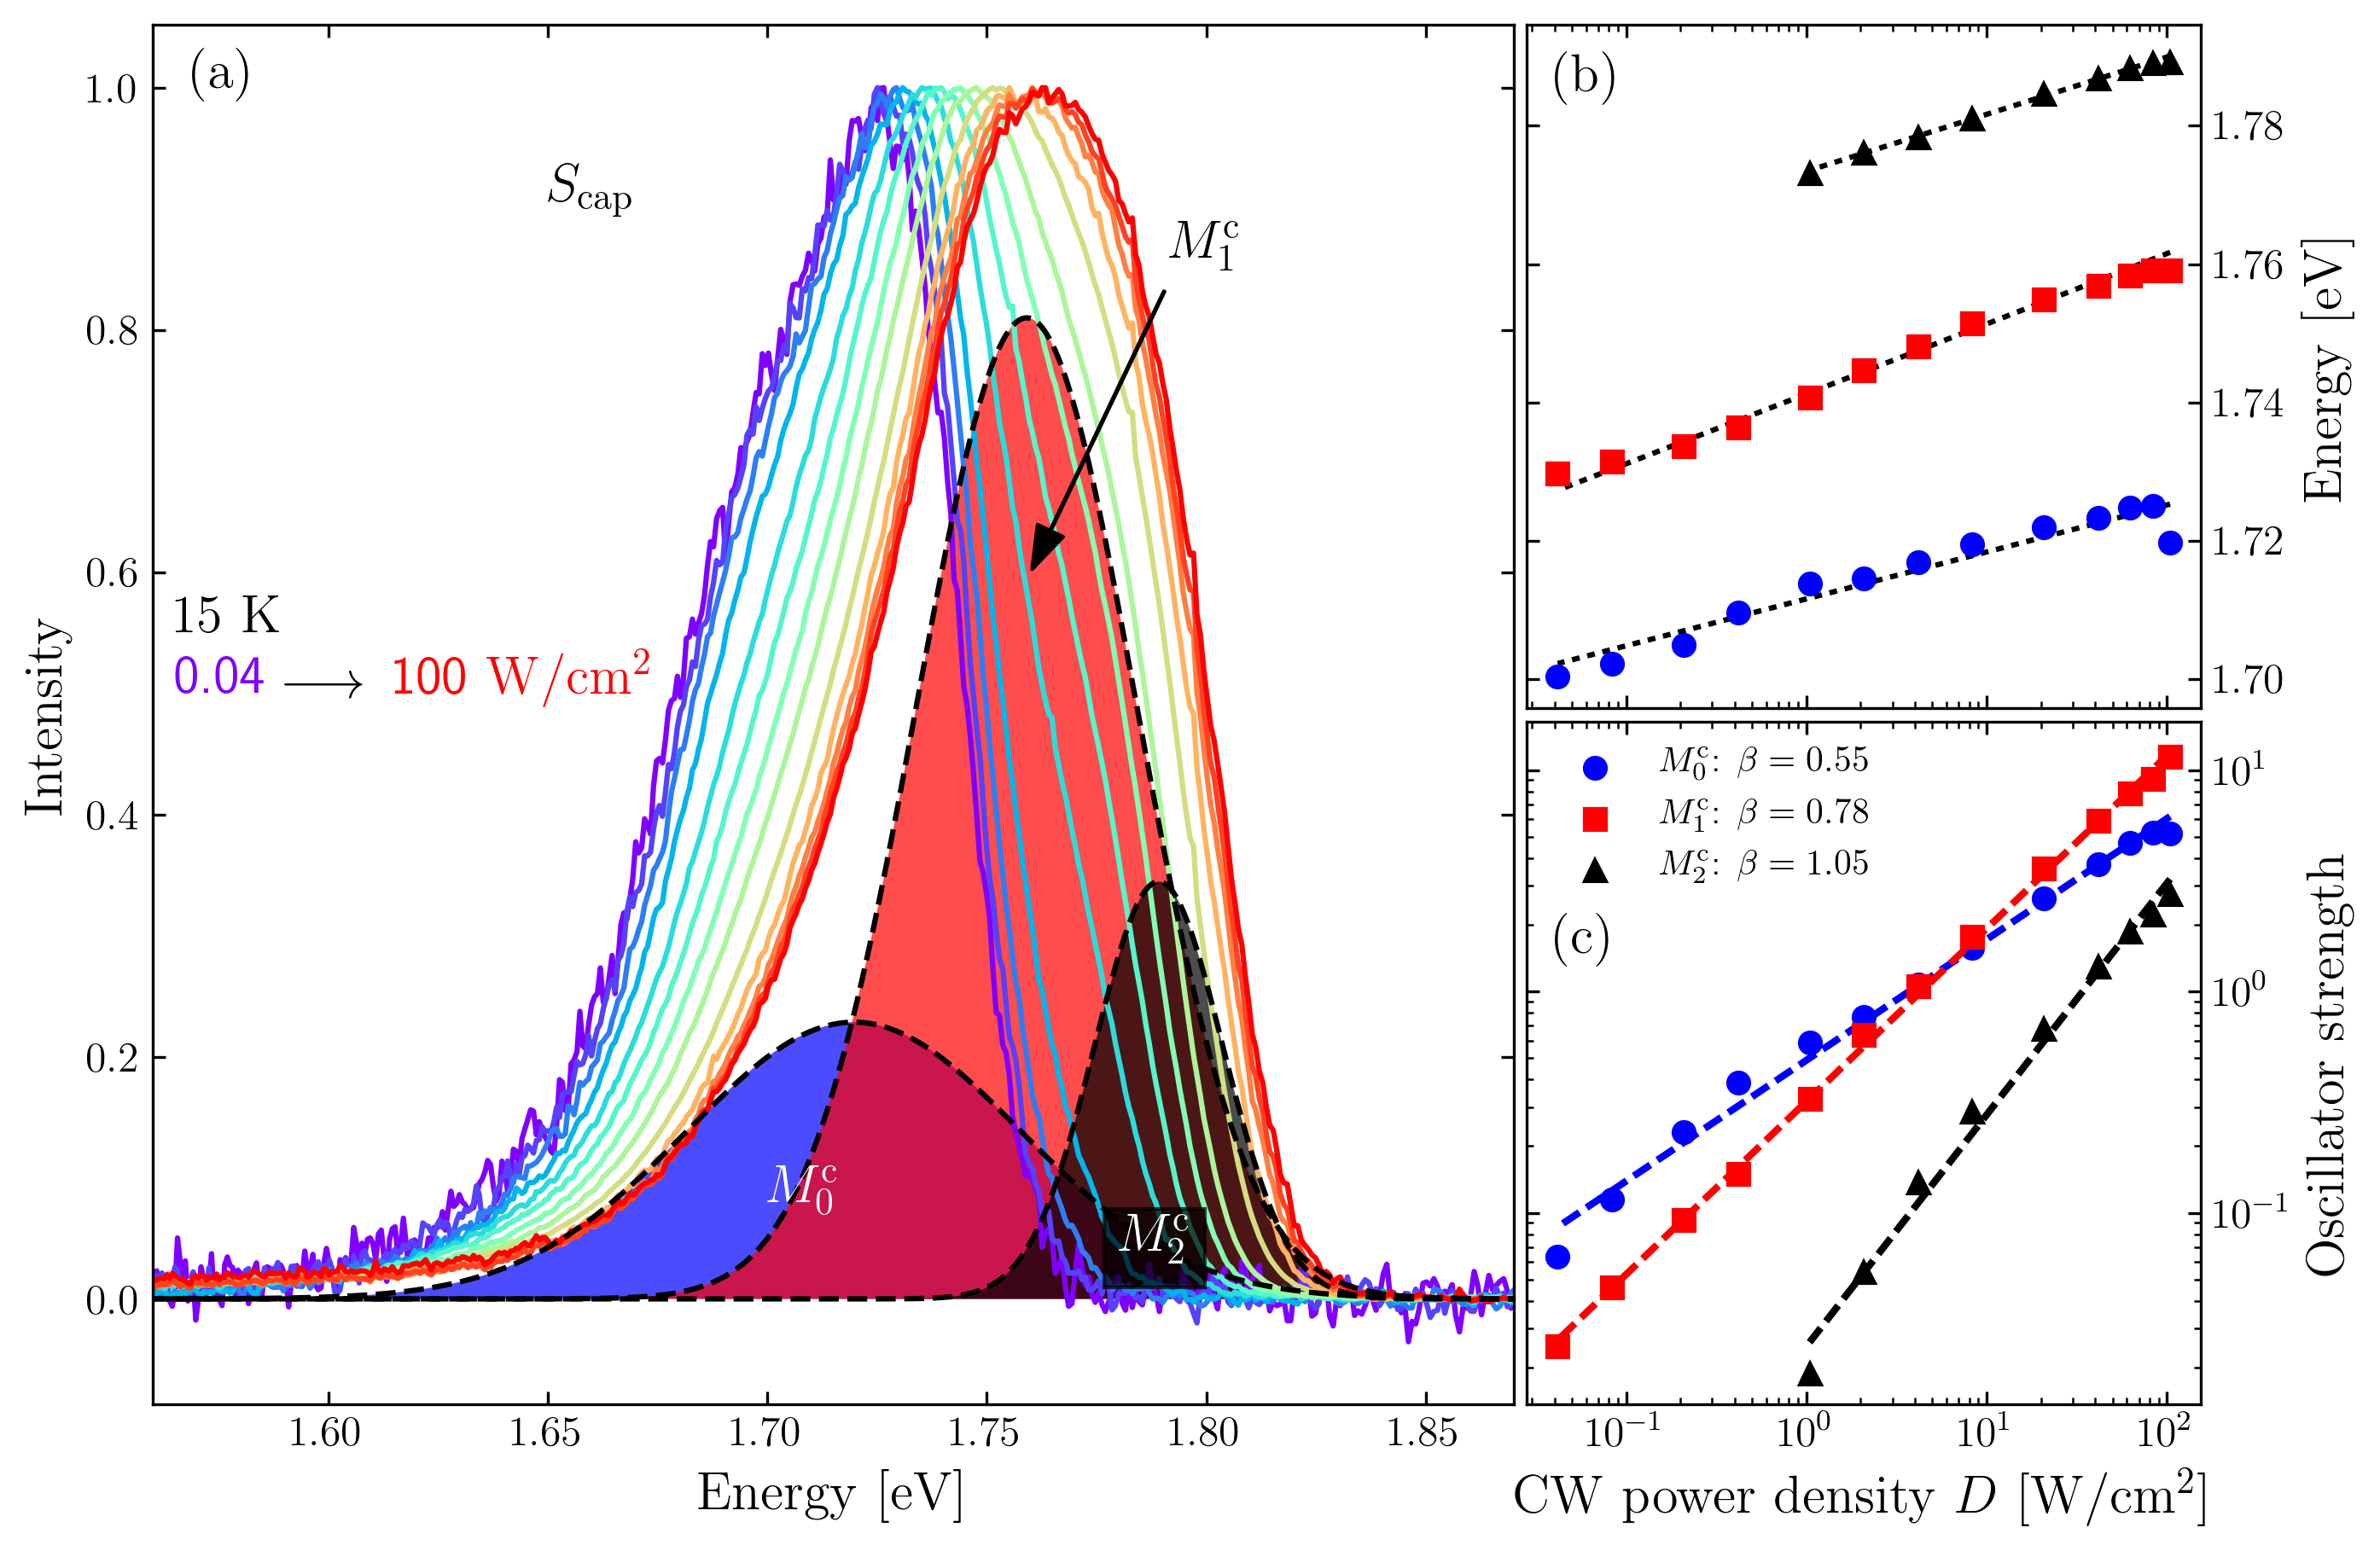
\includegraphics[width=0.9\linewidth]{/PL/intensity/12021_1108_norm_PL_int_typIvsII}
	\caption{The results are given in the same nomenclature as in Fig.~\ref{fig:QD_w_int}.}
	\label{fig:QD_cap_int}
\end{figure}

Intensity-resolved PL spectra of ${S_\mathrm{cap}}$ were treated similarly as for sample ${S_\mathrm{with}}$ and can be seen in Fig.~\ref{fig:QD_cap_int}. All of the bands have type-I band alignment. All fitted parameters are summarized in Tab.~\ref{tab:int_params}.
\begin{table}
	\centering
	\caption{Summary of the fitting parameters of power density dependent PL for all samples.}
	\begin{tabularx}{0.9\textwidth}{cCCcc}
		\toprule
		
		transition & $E_\mathrm{I}$ [meV]&  $U_\mathrm{e}+U_\mathrm{h}$ [meV]  & $\gamma$ [$\mathrm{meV W^{-1/3}cm^{2/3}}$] & $\beta$ \\ 	
		\midrule
		\midrule
		$M_0^\mathrm{w/o}$& $1819\pm1$ & $-0.02\pm 0.06$ & $0$& $0.55\pm0.02$\\
		$M_1^\mathrm{w/o}$& $1831\pm1$ & $1.0\pm0.1$ & $0$&  $0.79\pm0.02$\\
		$M_2^\mathrm{w/o}$ & $1859\pm2$ & $1.0\pm0.2$ & $3\pm2$&  $0.66\pm0.03$\\ 
		
		\midrule
		$M_0^\mathrm{w}$& $1735\pm2$ & $2\pm1$ & $6\pm2$&  $0.76\pm0.06$\\
		$M_1^\mathrm{w}$& $1772\pm4$ & $7\pm2$ & $0$&  $0.97\pm0.02$\\ %gamma=1\pm408e-5
		$M_2^\mathrm{w}$ &$1801\pm3$& $7\pm1$  &$0$ &$0.67\pm0.03$\\ %gamma=0.1\pm250e-5
		
		\midrule
		$M_0^\mathrm{c}$& $1712\pm2$ &   $3\pm1$& $0$  &$0.54\pm0.02$\\ %gamm=1\pm166 e-5
		$M_1^\mathrm{c}$& $1741\pm1$ & $4.4\pm0.6$ & $0$& $0.78\pm0.01$\\ %gamma=4\pm 112 e-5
		$M_2^\mathrm{c}$ & $1773\pm3$ & $3.6\pm0.5$ & $0$&  $1.05\pm0.04$\\ %gamma=4\pm53 e-5
		
		\bottomrule
	\end{tabularx}\label{tab:int_params}
\end{table}



%\begin{table}
%	\centering
%	\caption{Summary of the fitting parameters of power density dependent PL for all samples.}
%	\begin{tabularx}{0.9\textwidth}{cCCcc}
%		\toprule
		
%		transition & $E_\mathrm{I}$ [meV]&  $U_\mathrm{e}+U_\mathrm{h}$ [meV]  & $\gamma$ [$\mathrm{meV W^{-1/3}cm^{2/3}}$] & Type \\ 	
%		\midrule
%		\midrule
%		$M_0^\mathrm{w/o}$& $1819\pm1$ & $-0.02\pm 0.06$ & $0$& Type-I\\
%		$M_1^\mathrm{w/o}$& $1831\pm1$ & $1.0\pm0.1$ & $0$& Type-I\\
%		$M_2^\mathrm{w/o}$ & $1859\pm2$ & $1.0\pm0.2$ & $3\pm2$&  Type-II\\ 
		
%		\midrule
%		$M_0^\mathrm{w}$& $1735\pm2$ & $2\pm1$ & $6\pm2$&  Type-II\\
%		$M_1^\mathrm{w}$& $1772\pm4$ & $7\pm2$ & $0$&  Type-I\\ %gamma=1\pm408e-5
%		$M_2^\mathrm{w}$ &$1801\pm3$& $7\pm1$  &$0$ &Type-I\\ %gamma=0.1\pm250e-5
%		
%		\midrule
%		$M_0^\mathrm{c}$& $1712\pm2$ &   $3\pm1$& $0$  &Type-I\\ %gamm=1\pm166 e-5
%		$M_1^\mathrm{c}$& $1741\pm1$ & $4.4\pm0.6$ & $0$& Type-I\\ %gamma=4\pm 112 e-5
%		$M_2^\mathrm{c}$ & $1773\pm3$ & $3.6\pm0.5$ & $0$&  Type-I\\ %gamma=4\pm53 e-5
		
%		\bottomrule
%	\end{tabularx}\label{tab:int_params}
%\end{table}


The evolution of the emission bands of sample $S_\mathrm{cap}$ with excitation intensity is compared with predictions obtained within the semi-self-consistent CI (SSCCI) presented in Ref.~\citep{Klenovsky2017} %and described in chapter~\ref{chap:SciRep} 
for 2.5~nm height In$_{0.15}$Ga$_{0.85}$As$_{0.85}$Sb$_{0.15}$/GaAs/GaP QD by the supervisor. The band $M_1^\mathrm{c}$ is reasonably well reproduced by SSCCI with basis formed from single-particle wavefunctions calculated by $1\times8~\mathbf{k \cdot p}$ method with electrons originating from $L$ and holes form $\Gamma$-point. On the other hand, SSCCI with $8\times8~\mathbf{k \cdot p}$ basis for electrons coming from $\Gamma$-point can desbribe the band $M_2^\mathrm{c}$.
\begin{figure}
	\centering
	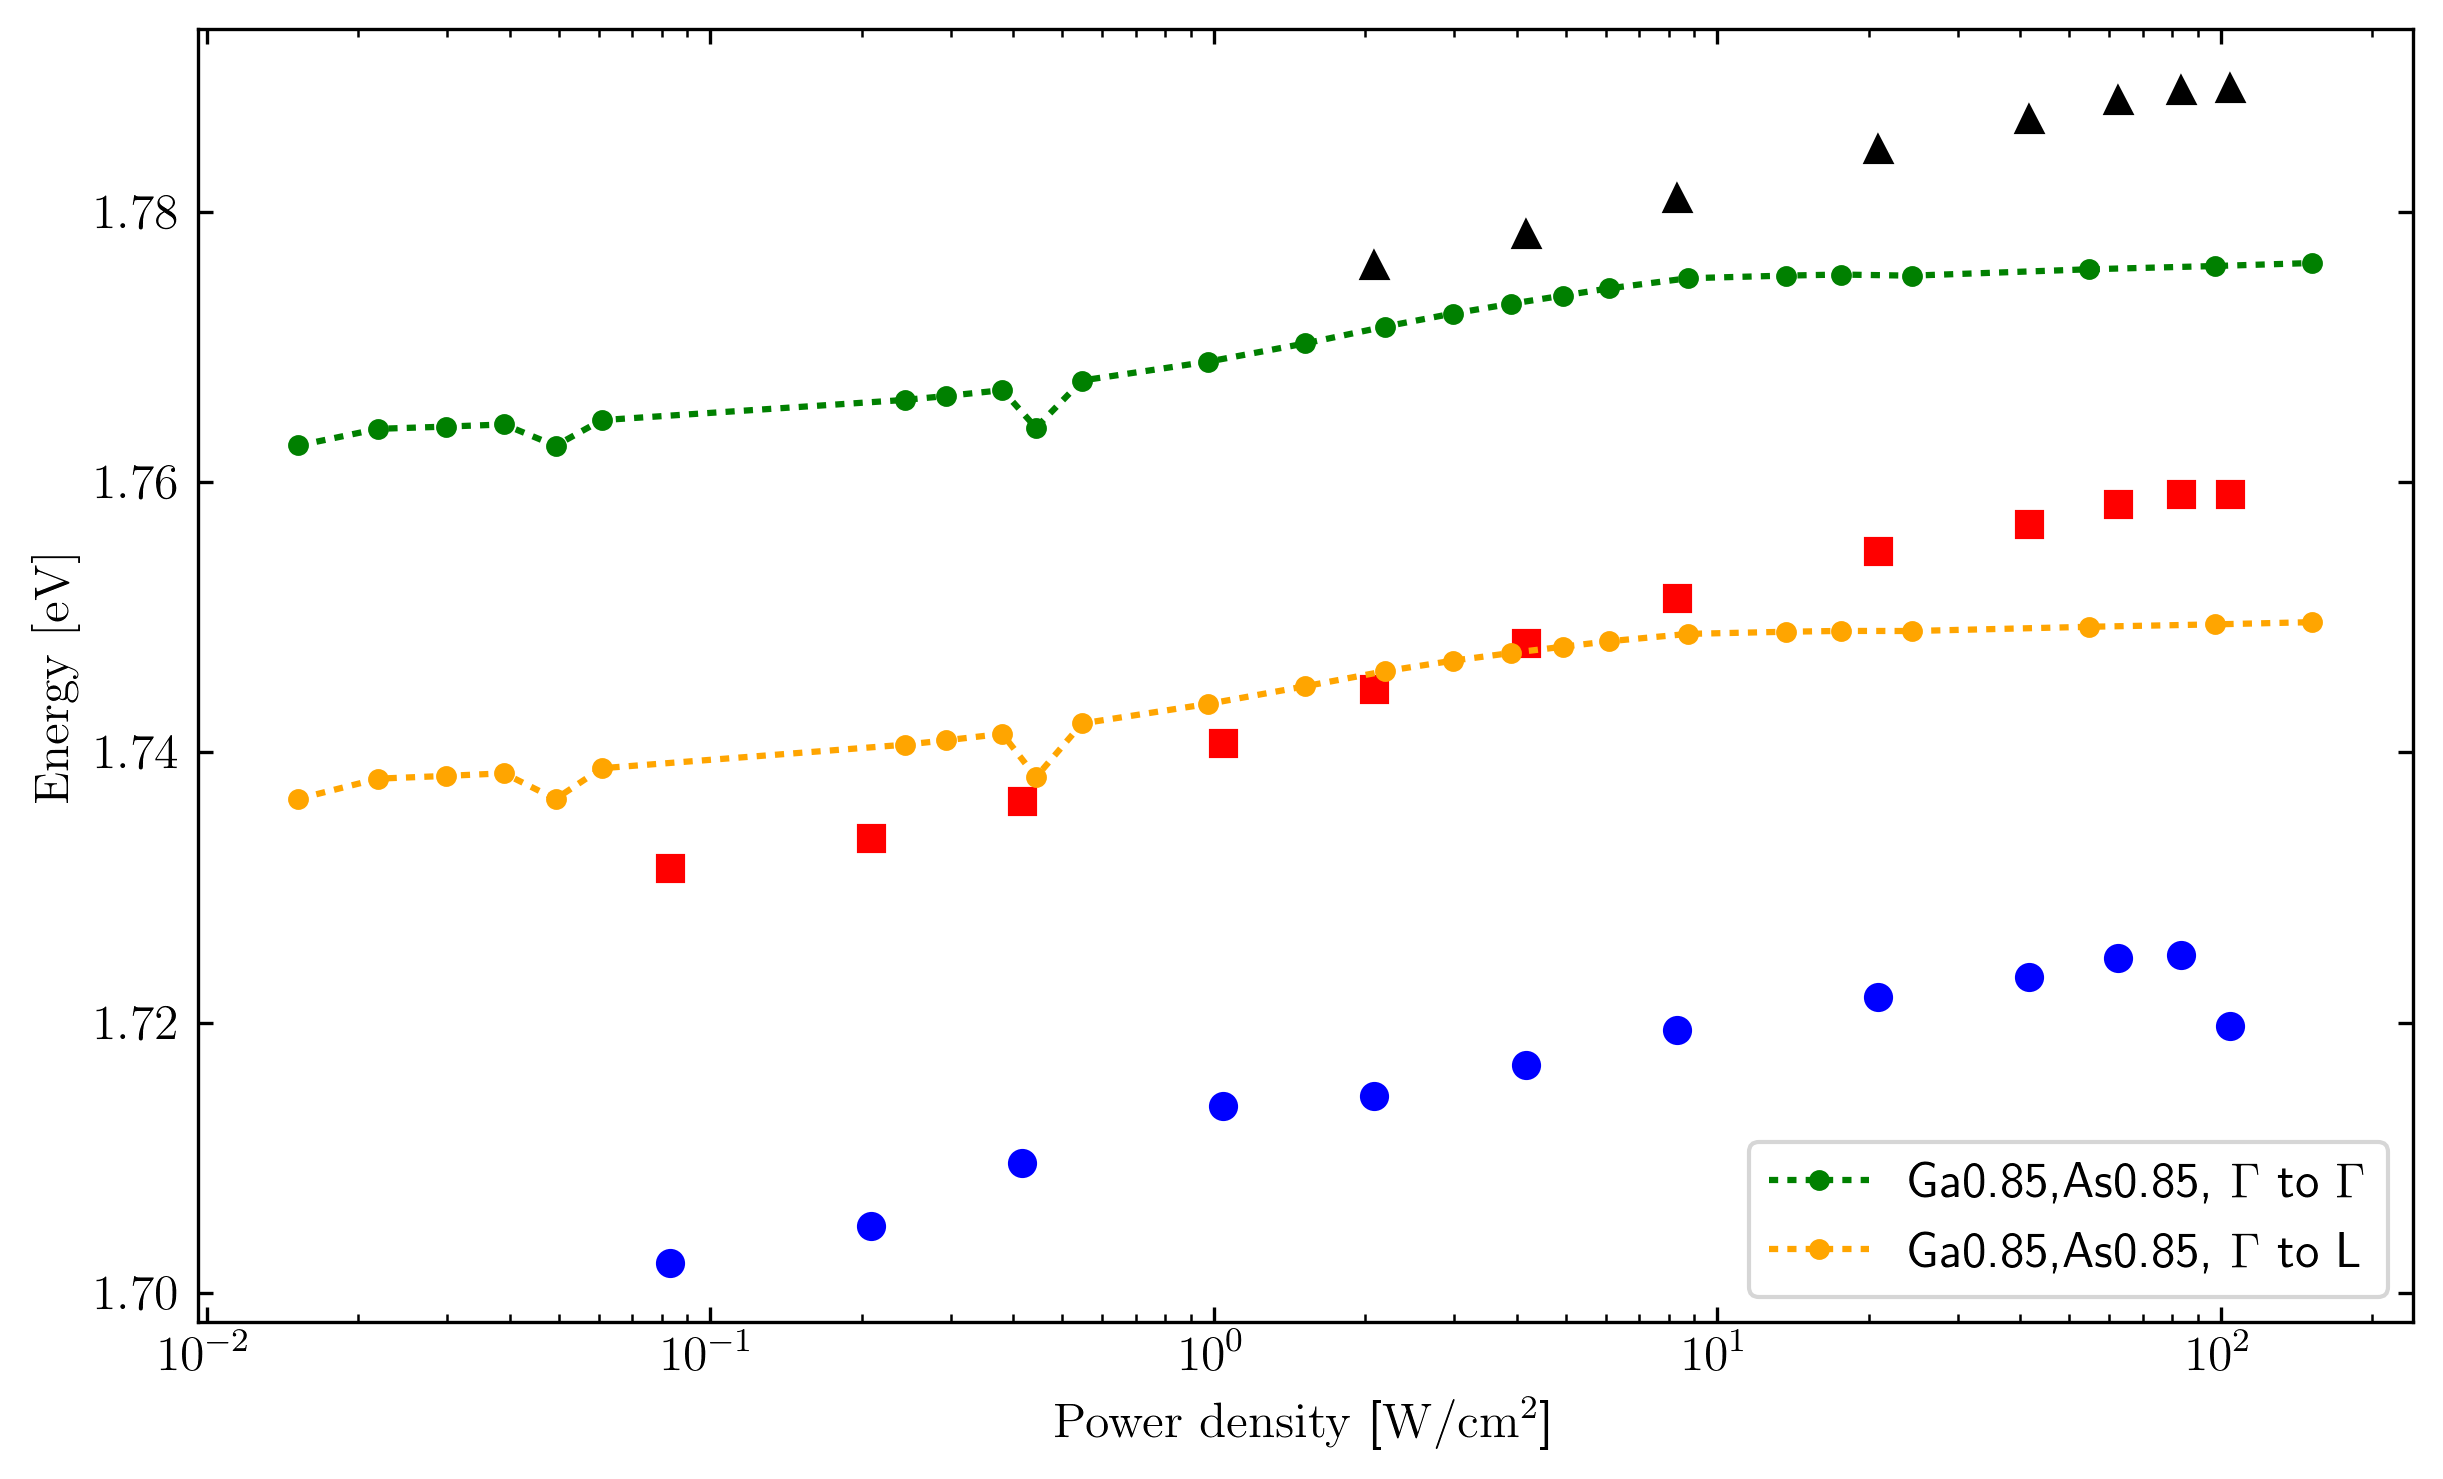
\includegraphics[width=0.9\linewidth]{/PL/intensity/S_cap_expvskpcalc}
	\caption{Emission energy evolution with excitation intensity predicted by SSCCI with single-particle bases calculated by $1\times8~\mathbf{k \cdot p}$ and $8\times8~\mathbf{k \cdot p}$, respectively (dotted curve). To compare experimental points are added.}
	\label{fig:QD_cap_int_expvstheory}
\end{figure}

\newpage
\subsection{Temperature dependent PL}
\label{Sec:temp_PL_TU}
The temperature dependences of the PL of the studied samples was fitted by three Gaussian profiles as in the excitation density investigation in Sec.~\ref{sec:intensity_PL_TU}. The fitted energies were examined using the Varshni-like model
%
\begin{equation}
E(T)=E_0-\frac{\alpha T^2}{T+\Theta_\mathrm{D}}-\frac{\sigma^2}{k_\mathrm{B}T}, \label{eq:Varshni-like}
\end{equation}
where $E_0$ is the energy at temperature $T=0~\mathrm{K}$, $\alpha$ and $\Theta_\mathrm{D}$ are the Varshni parameters, $k_\mathrm{B}$ is Boltzmann constant. The model provides the thermally dependent correction of the empirical Varshni model~\citep{Varshni} describing temperature effects to a band gap of an idealized bulk semiconductor. The estimation proposed by Eliseev~\citep{Eliseev_apl2003_PLtemp} to evaluate the correction is used, which assumes the Gaussian-type distribution of energy of the localized states with broadening parameter $\sigma$.

The mechanisms responsible for the temperature quenching of PL intensity can be accounted for by a Boltzmann model for excitonic recombination with two characteristic activation energies~\citep{Daly_prb1995, Alen_apl2011}
\begin{equation}
I_\mathrm{PL}(T)=\frac{I_0}{1+\tau_0\left[\Gamma_1\exp(-E_1/k_\mathrm{B}T)+\Gamma_2\exp(-E_2/k_\mathrm{B}T)\right]},               \label{eq:Arhenius}
\end{equation}
where $I_0$ is the intensity at 0~K, $\tau_0$ temperature-independent radiative recombination time at 15~K, $E_1$ and $E_2$ are the activation energies of the two quenching mechanisms with related scattering rates $\Gamma_1$ and $\Gamma_2$.%These parameters are representative of the average behaviour of the emissions bands, being the most important $\tau_0$, $E_1$ and $E_2$.
\newpage
\subsubsection*{Sample without QDs $\mathbf{S_\mathrm{w/o}}$}
%
Three recognized emission bands ($M_0^\mathrm{w/o}$, $M_1^\mathrm{w/o}$ and $M_2^\mathrm{w/o}$) in PL of ${S_\mathrm{w/o}}$ are individually investigated from 15~K to 220~K. In this range we can observe Varshni energy-shift of $M_1^\mathrm{w/o}$ and $M_2^\mathrm{w/o}$ described by parameters listed in Tab.~\ref{tab:Varshni}, see Fig.~\ref{fig:QD_wo_temp}(b). In Fig.~\ref{fig:QD_wo_temp}(c) intensity quenching through the temperature range evaluated by the Boltzmann model~(\ref{eq:Arhenius}) is depicted.
%
\begin{figure}
	\centering
	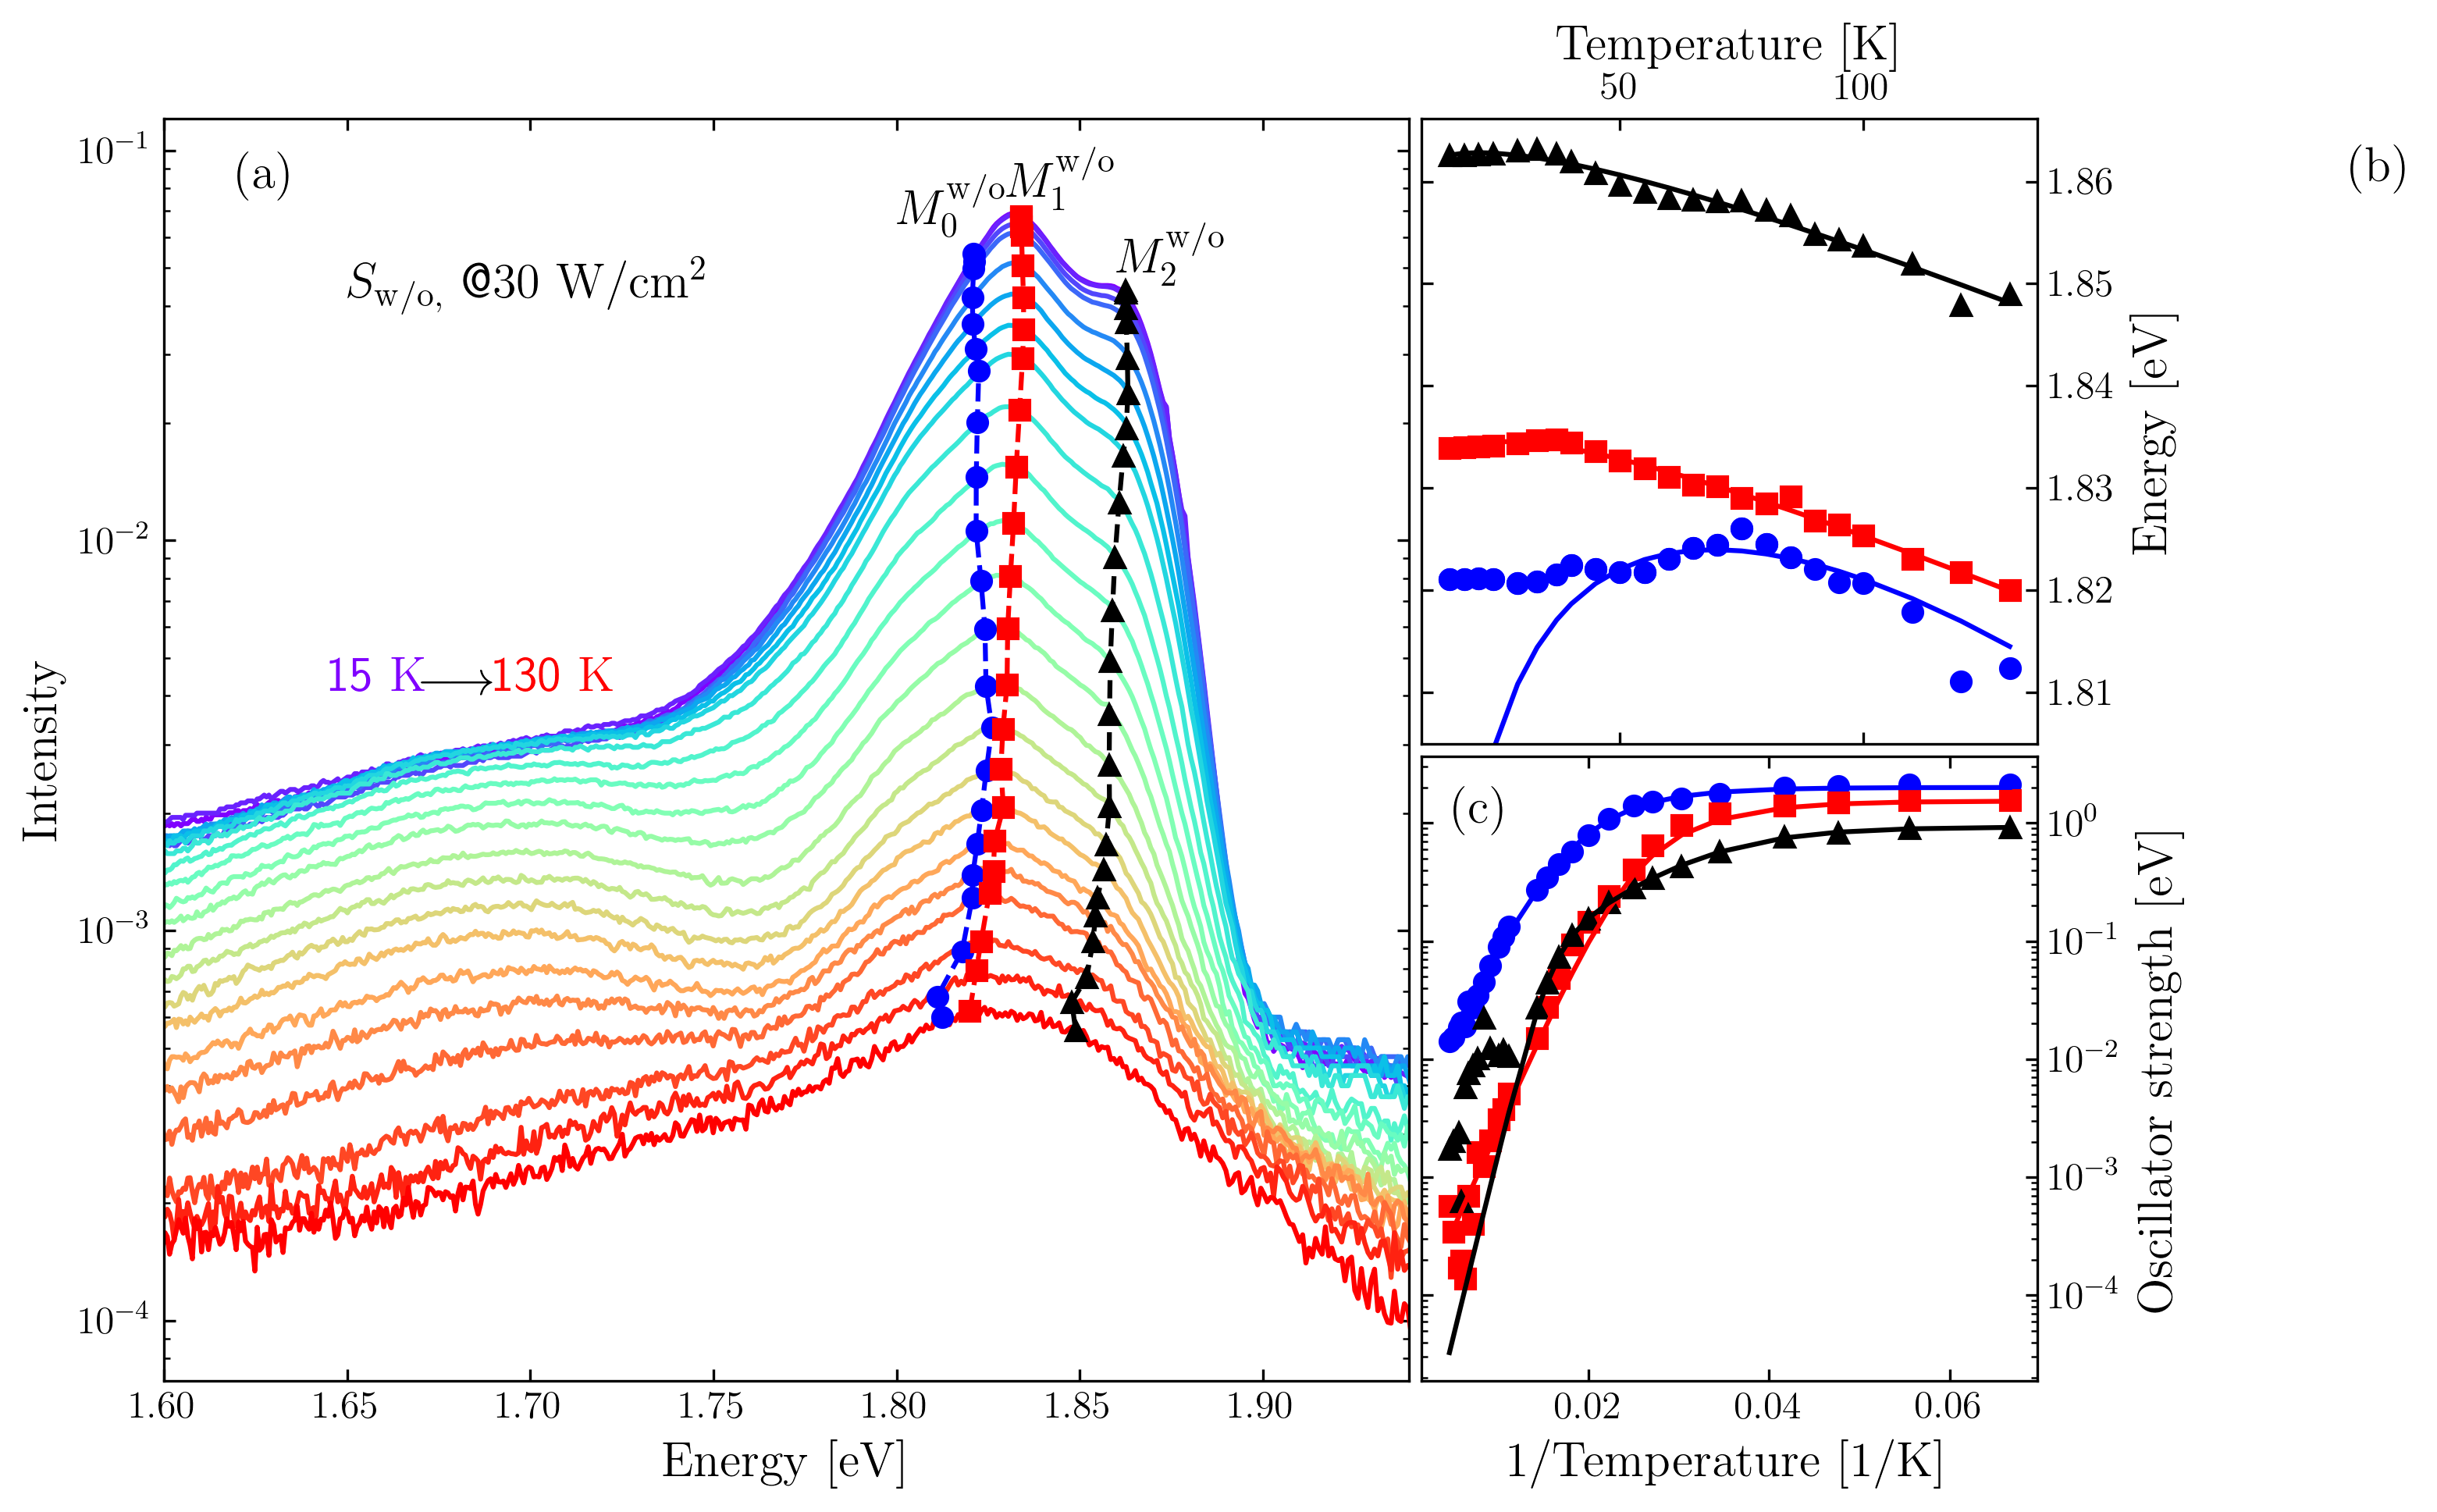
\includegraphics[width=0.9\linewidth]{/PL/temperature/12027_7mW_log_PL_int_without}
	\caption{(a) PL spectra of sample $S_\mathrm{w/o}$ measured at 30~W/cm$^2$ excitation density in 15-220~K temperature range. Each spectrum is fitted by a sum of three Gaussian profiles represented by symbols in panel (a): $M_0^\mathrm{w/o}$ blue circles, $M_1^\mathrm{w/o}$ red squares and $M_2^\mathrm{w/o}$ black triangles. The bands are similarly marked in panels (b) and (c) where also the experimental transition energies (symbols) and fits by the Varshni model~(\ref{eq:Varshni-like}) (lines), respectively, and the integrated PL intensity (symbols) fitted by the Boltzmann model~Eq.~(\ref{eq:Arhenius}) are presented. All fitting parameters are listed in Tabs.~\ref{tab:Varshni} and~\ref{tab:Arhenius}.}
	\label{fig:QD_wo_temp}
\end{figure}


\subsubsection*{Sample with QDs $\mathbf{S_\mathrm{with}}$}
%
In temperature range between 15 and 150~K we observe quenching of PL intensity of three optical transitions marked $M_0^\mathrm{w}$, $M_1^\mathrm{w}$ and $M_2^\mathrm{w}$, see Fig.~\ref{fig:QD_w_temp}(a). The transition energies (Fig.~\ref{fig:QD_w_temp}(b)) and the oscillator strengths (Fig.~\ref{fig:QD_w_temp}(c)) are fitted by the Varshni model~Eq.~(\ref{eq:Varshni-like}) and the Boltzmann model~Eq.~(\ref{eq:Arhenius}) in the whole measured temperature range.  
%
\begin{figure}
	\centering
	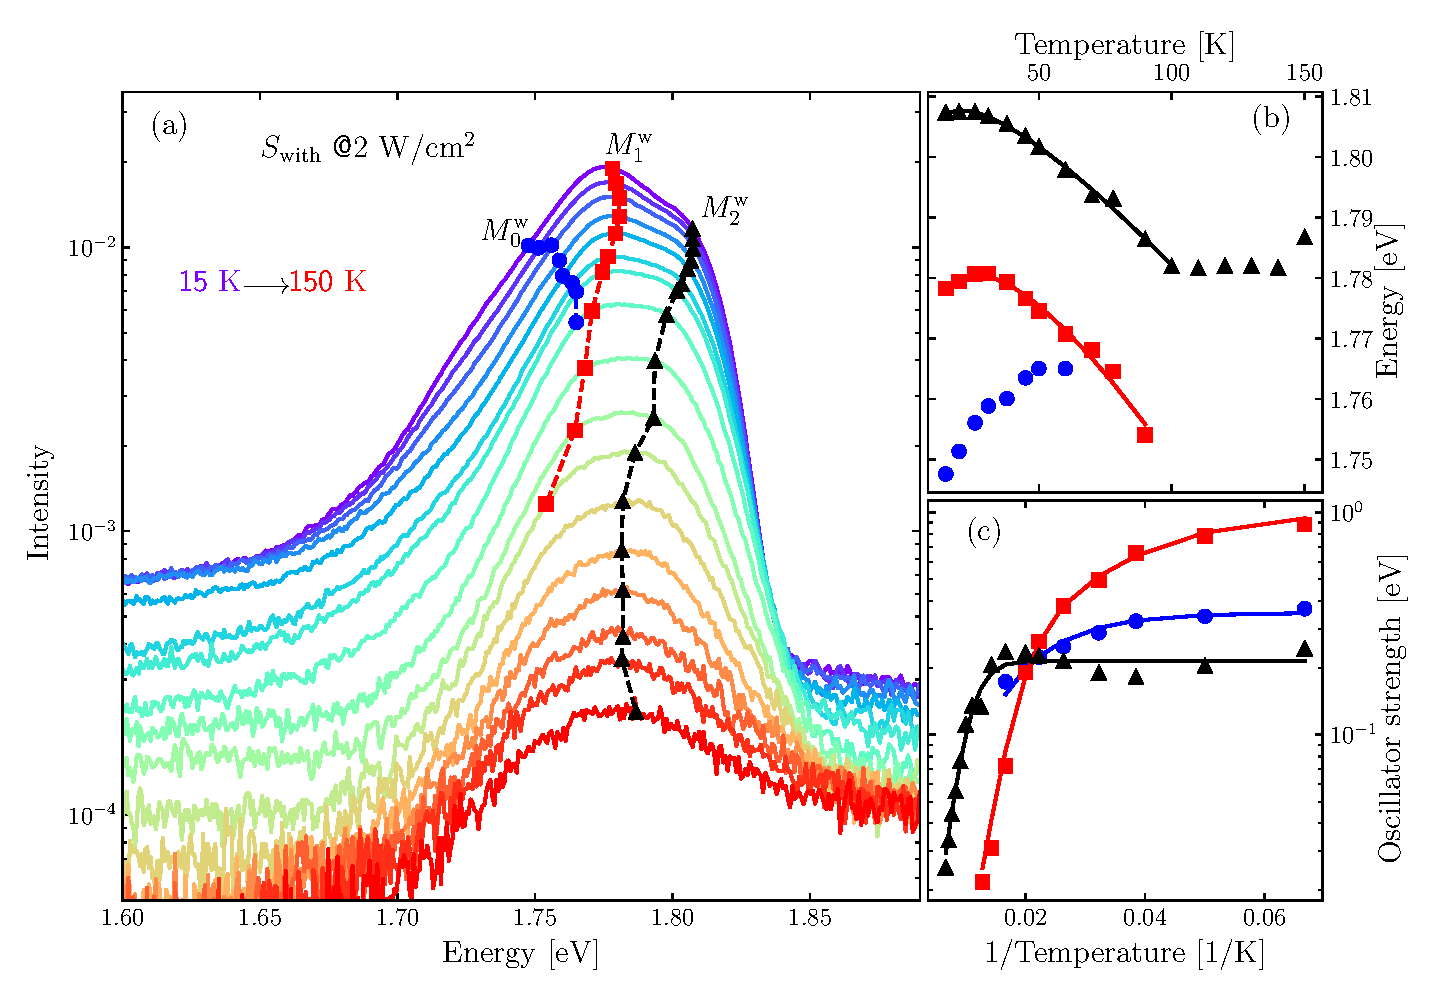
\includegraphics[width=0.9\linewidth]{/PL/temperature/12040_500uW_log_PL_int_Varshni}
	\caption{PL spectra of the sample ${S_\mathrm{with}}$ at 2~W/cm$^2$ between 15 and 150~K. The results are given in the same way as in Fig.~\ref{fig:QD_wo_temp}.}
	\label{fig:QD_w_temp}
\end{figure}

\newpage
\subsubsection*{Sample with capped QDs $\mathbf{S_\mathrm{cap}}$}
%
PL spectra of ${S_\mathrm{cap}}$ are deconvoluted into three bands ($M_0^\mathrm{c}$, $M_1^\mathrm{c}$ and $M_2^\mathrm{c}$) and investigated in temperature range 15-110~K, see Fig.~\ref{fig:QD_c_temp}.
%
\begin{figure}[h]
	\centering
	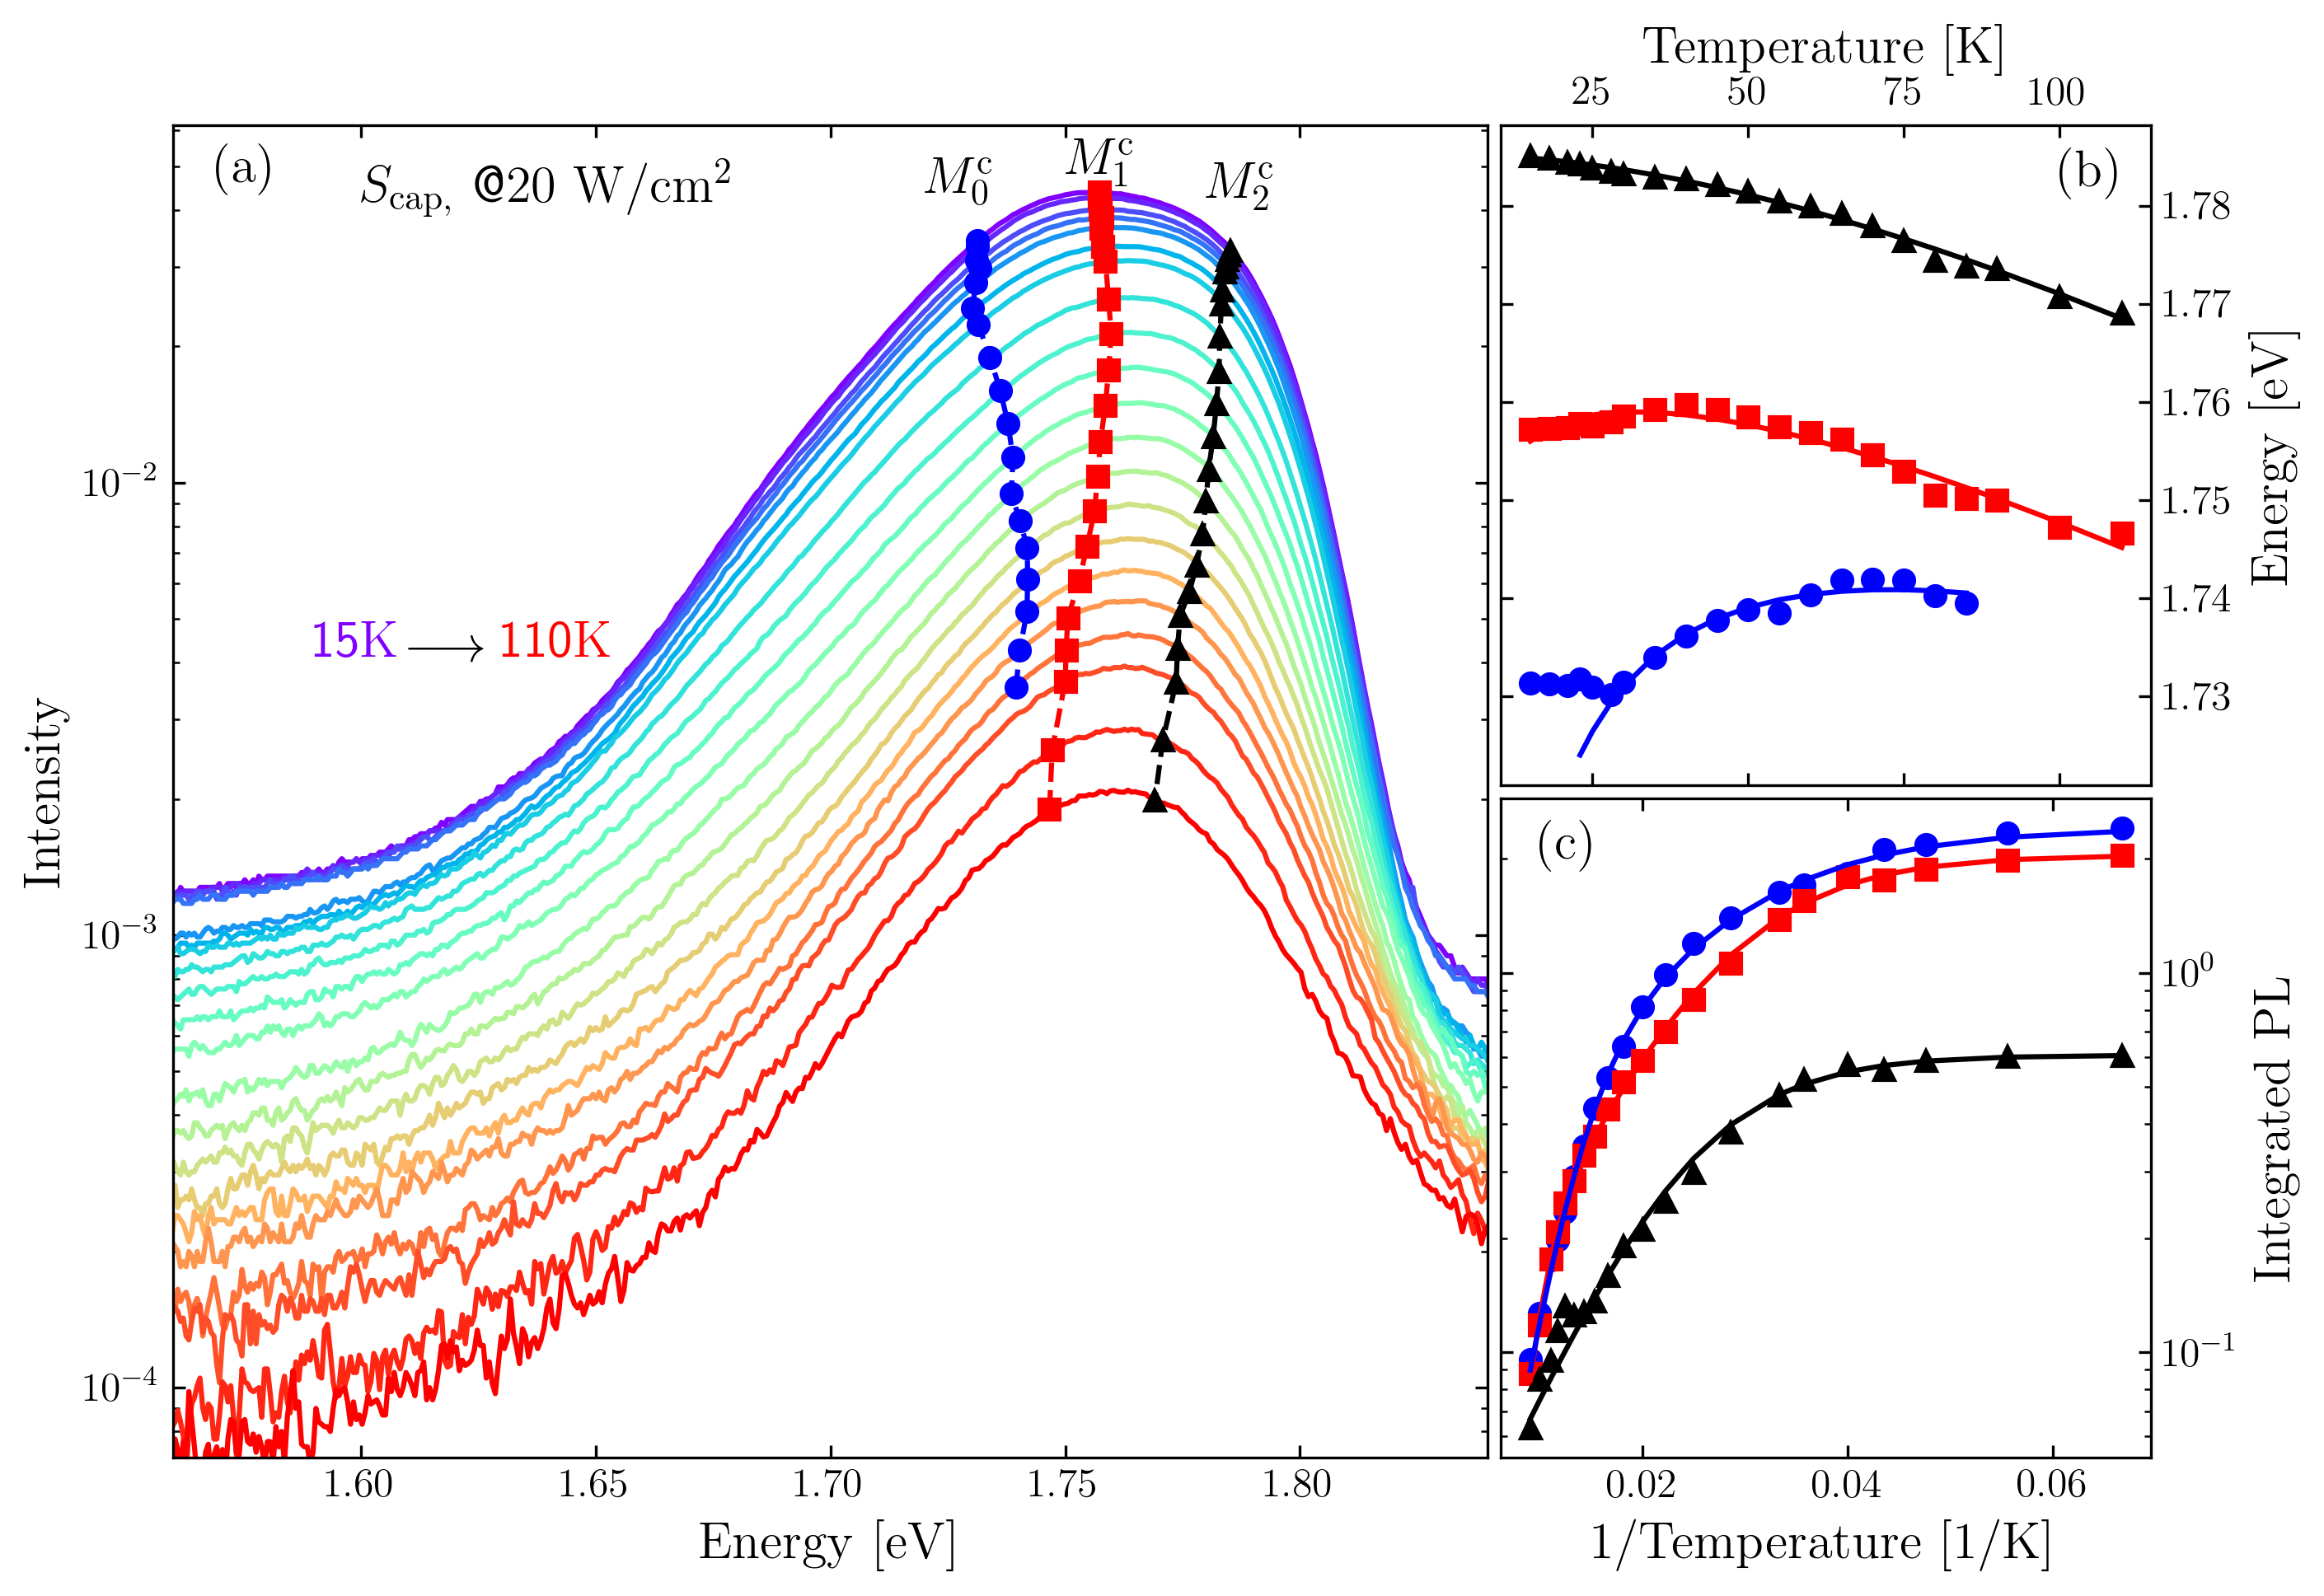
\includegraphics[width=0.9\linewidth]{/PL/temperature/12021_5mW_log_PL_int_Varshni}
	\caption{PL spectra of the sample ${S_\mathrm{cap}}$ measured at 20~W/cm$^2$ between 15 and 110~K. The results are given in the same nomenclature as in Fig.~\ref{fig:QD_wo_temp}.}
	\label{fig:QD_c_temp}
\end{figure}

\newpage
\subsubsection*{Discussion of temperature resolved PL results}
The value of $E_1$ (4--15~meV) is comparable for all samples and also for every PL bands. This low activation energy is determining the low-temperature quenching of the PL and it is usually associated to carrier recombination through impurities. The values of the high-temperature quenching $E_2$ (29--43~meV) are also similar across the samples except the deviation in $M_2^\mathrm{c}$ where we measured extremely small activation energy ($E_2=1$~meV) and $M_2^\mathrm{w/o}$ with $E_2$ twice larger than for other bands ($E_2=62$~meV).

\begin{figure}
	\centering
	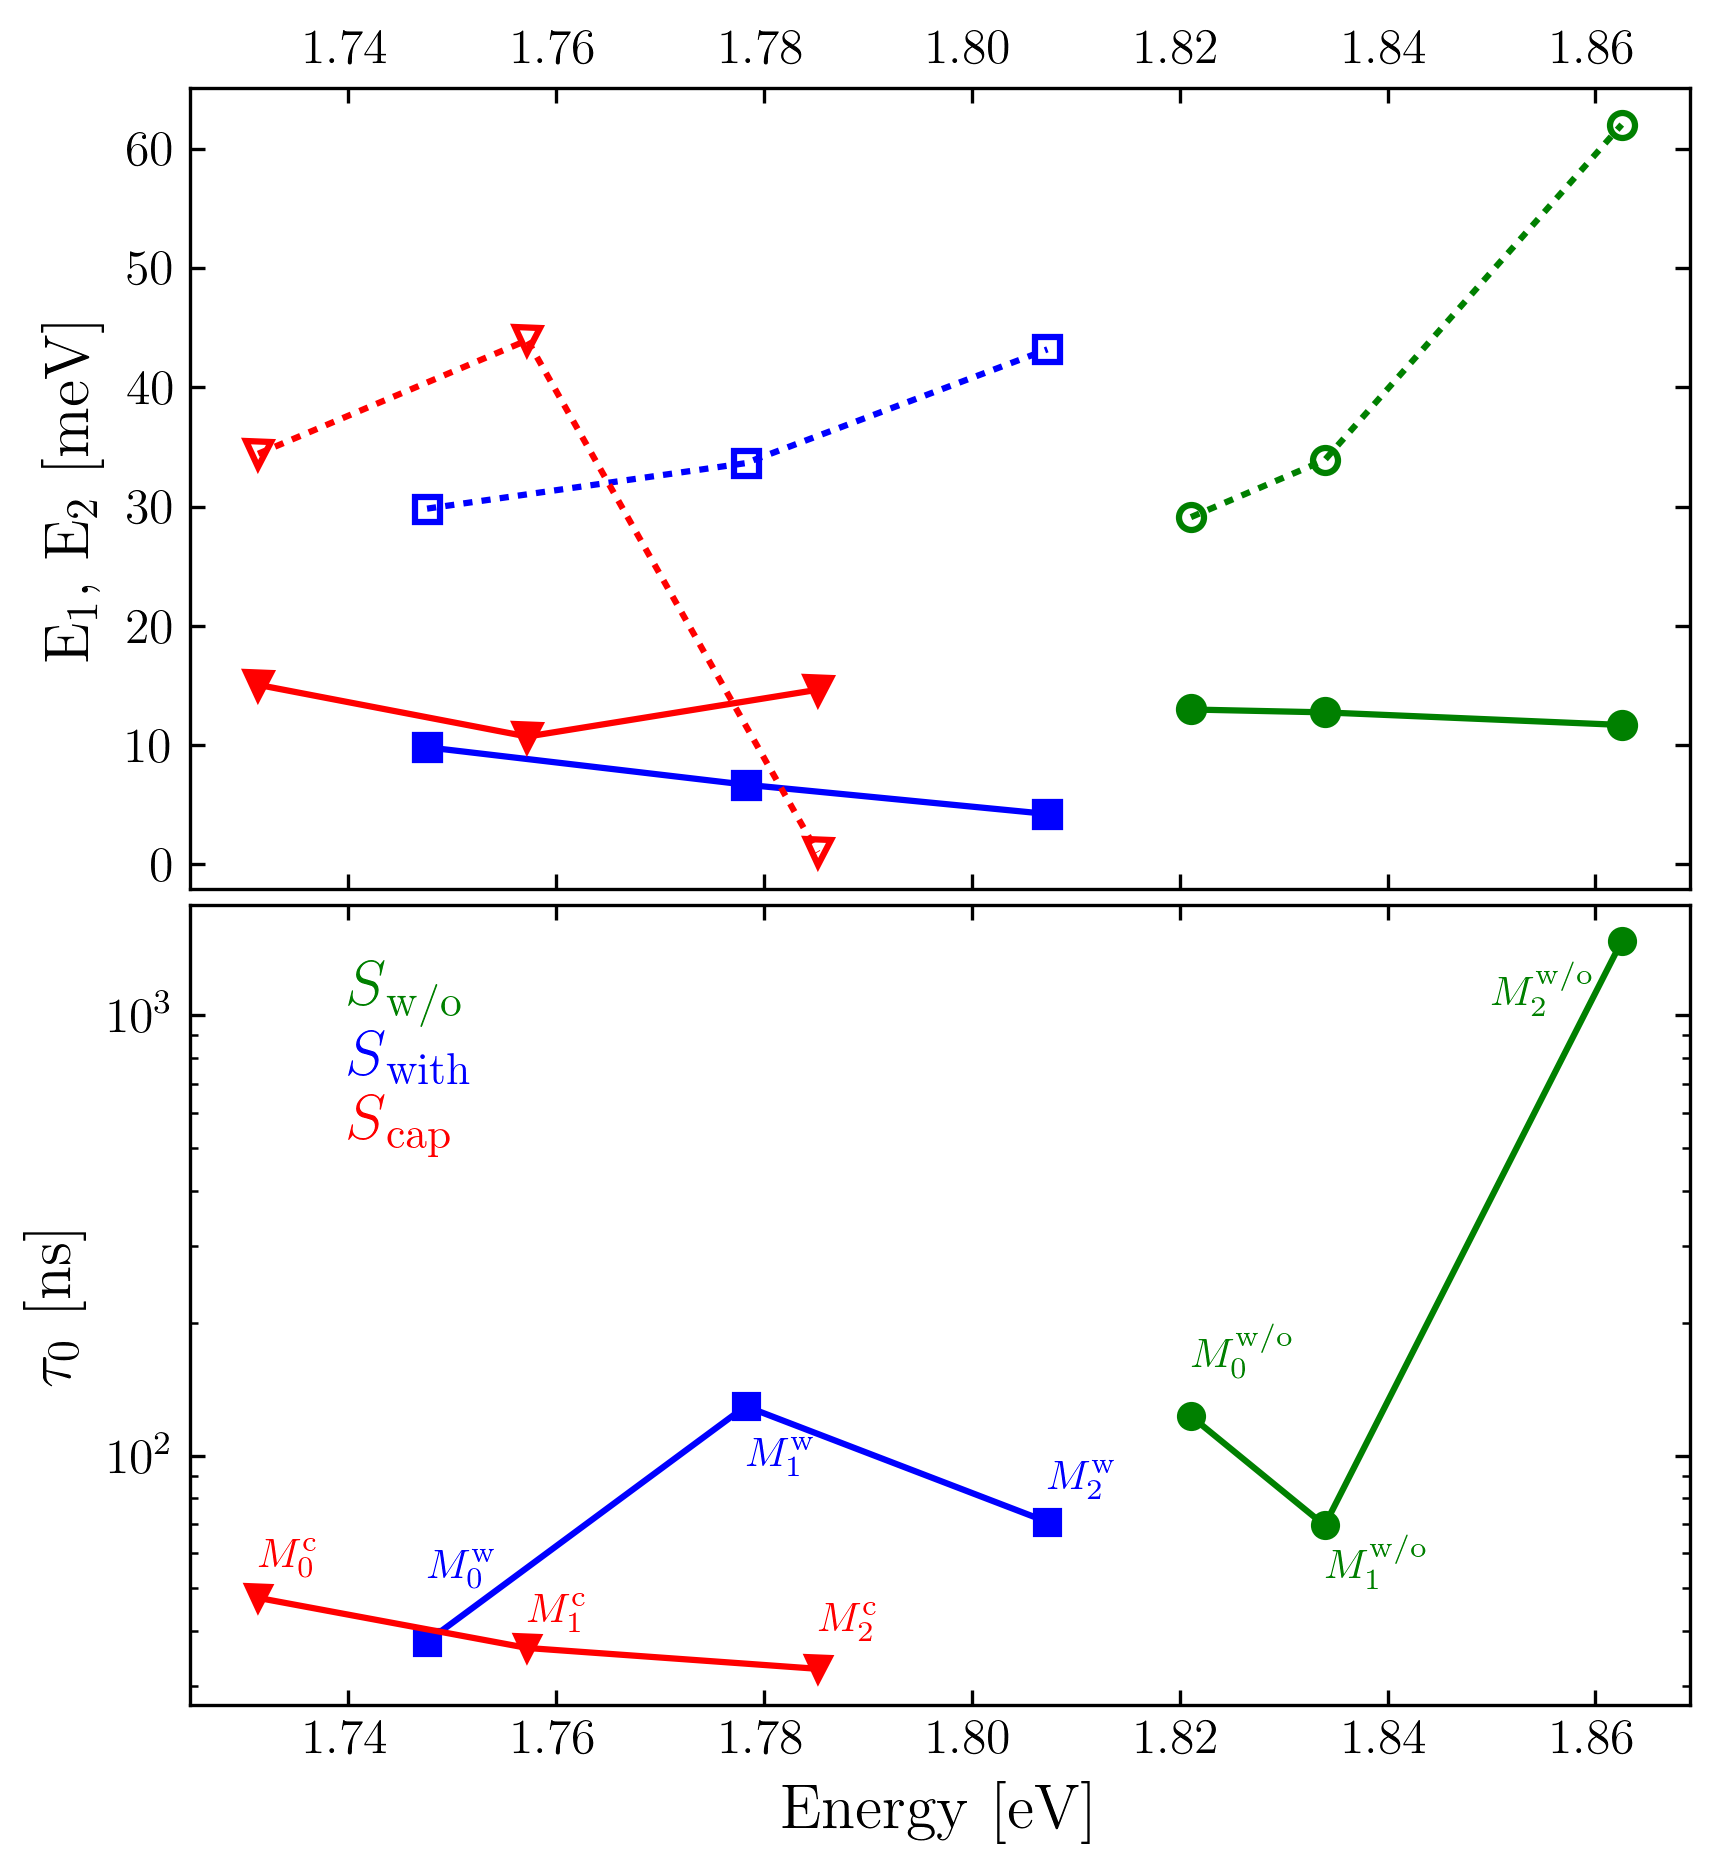
\includegraphics[width=0.75\linewidth]{/PL/temperature/all_Arhenius}
	\caption{Comparison of the Boltzmann fitting parameters for the studied samples. The upper panel depicts $E_1$ (empty symbols) and $E_2$ (full symbols), respectively, the bottom panel shows $\tau_0$. Samples are distinguished by the type and colour of symbols as in Fig.~\ref{fig:PL_homogenity}.}
	\label{fig:Arrhenius_all}
\end{figure}


\begin{table}
	\centering
	\caption{Summary of the Varshni-like fits. The accuracy of $E_0$ and $\alpha$ are better than $10^{-4}\%$, and better than 5~\% for $\Theta_\mathrm{D}$ and $\sigma$.}
	\begin{tabularx}{0.9\textwidth}{cCCcc}
		\toprule
		
		transition & $E_0$ [meV]& $\alpha$ [$10^{-4}~\mathrm{eVK^{-1}}$]& $\Theta_\mathrm{D}$ [K]& $\sigma$ [meV]\\ 	
		\midrule
		\midrule
		$M_0^\mathrm{w/o}$& $1845$ & $7.99$& $450$&$9.1$\\
		$M_1^\mathrm{w/o}$& $1838$ & $2.14$& $67$&$2.4$\\
		$M_2^\mathrm{w/o}$ & $1865$ & $2.10$& $78$& $1.7$\\ 
		
		\midrule
		$M_0^\mathrm{w}$& $1789$ & $10.00$& $270$& $8.1$\\
		$M_1^\mathrm{w}$& $1789$ & $23.37$& $150.1$&$3.6$\\
		$M_2^\mathrm{w}$ & $1815$& $5.49$& $74.5$& $2.8$\\ 
		
		\midrule
		$M_0^\mathrm{c}$& $1756$ & $5.00$& $420$& $7.9$\\
		$M_1^\mathrm{c}$& $1766$ & $4.03$& $144.5$& $3.4$\\
		$M_2^\mathrm{c}$ & $1785$ & $4.90$& $243.2$& $1.7\cdot 10^{-5}\pm0.06$\\%$3.3\cdot 10^{-7}$\\
		
		\bottomrule
	\end{tabularx}\label{tab:Varshni}
\end{table}

\begin{table}
	\centering
	\caption{Summary of the Arhenius-like fits. The displayed values are obtained with accuracy better than $10^{-4}~\%$.}
	\begin{tabularx}{0.9\textwidth}{cCCcccc}
		\toprule
		
		%transition & $I_0$ & $\tau_0$ [ns]& $\Gamma_1$ [ns$^{-1}$]& $E_1$ [meV]& $\Gamma_2$ [ns$^{-1}$]& $E_2$ [meV]\\ 	
	%	\midrule
	%	\midrule
	%	$M_0^\mathrm{w/o}$& 7.65135744e-01&   65.2916823&   566.317577&  7.60337981&8.65963570&   27.3857198 \\
	%	$M_1^\mathrm{w/o}$& 4.38191968e-01&   92.4725944&   1.26183745&   15.1174840&   500.994206&   37.1135443\\
	%	$M_2^\mathrm{w/o}$ & 1.00415726e-11&   95.1667043&   34.0939008&   9.27548824&   96.6322136&   36.5620565\\ 
		
	%	\midrule
	%	$M_0^\mathrm{w}$& 3.53321027e-01&   37.8298857&   17.4314590&  9.81156539&   2.85772107 &  29.8347168\\
	%	$M_1^\mathrm{w}$& 9.99521298e-01 &  129.480243 &  864.188777 &  6.67625574&   39.7837356 &  33.6514094\\
	%	$M_2^\mathrm{w}$ & 2.15529619e-01&   70.7125983&   297.344867 &  4.21713415&   25.0223987 &  43.1983367\\ 
		
	%	\midrule
	%	$M_0^\mathrm{c}$& 2.40563456e+00&  47.5372923&   4.03965001&  34.4371546&   1.38672287&   15.0504481\\
	%	$M_1^\mathrm{c}$& 2.05316367e+00&   36.5787466&   81.4268881&   10.7120315&   19.2461237&  43.9676048\\
	%	$M_2^\mathrm{c}$ & 2.61200307e+00&   32.8025509 &  18.6448452 &  1.00000016&   5.01856897&  14.6371152\\
		
		
			transition & $I_0$ & $\tau_0$ [ns]& $\Gamma_1$ [ns$^{-1}$]& $E_1$ [meV]& $\Gamma_2$ [ns$^{-1}$]& $E_2$ [meV]\\ 	
			\midrule
			\midrule
			$M_0^\mathrm{w/o}$&  2.000 &  122.9&   13.17&  13.0&  4.62&   29.1 \\
			$M_1^\mathrm{w/o}$& 1.533&   69.5&  93.62&   12.7&   424.25&  33.9\\
			$M_2^\mathrm{w/o}$ &  0.925 &  1474.1 &  456.81 &  11.7&   506.20 &  62.1\\ 
			
			\midrule
			$M_0^\mathrm{w}$& 0.353&   37.8&   17.43&  9.8&   2.86 &  29.8\\
			$M_1^\mathrm{w}$& 0.999 &  129.5 &  864.19&  6.7&   39.78 &  33.7\\
			$M_2^\mathrm{w}$ & 0.216&   70.7&   297.34 &  4.2&   25.02&  43.2\\ 
			
			\midrule
			$M_0^\mathrm{c}$& 2.406&  47.5&   1.39&   15.0 &   4.04&  34.4\\
			$M_1^\mathrm{c}$& 2.053&   36.5&   81.43&   10.7&   19.25&  44.0\\
			$M_2^\mathrm{c}$ & 2.612&   32.8&   5.02&  14.6 &  18.65 &  1.0\\
			
		\bottomrule
	\end{tabularx}\label{tab:Arhenius}
\end{table}


\clearpage
\subsection{Polarization dependent PL }
In our experiments, both the excitation and the detected PL radiation propagate perpendicularly to the sample surface; the angle between the crystallographic direction~[110] and the polarization vector is denoted $\theta$. Because low degrees of polarization of the emitted light is expected, we visualize our experimental results in terms of the degree of polarization
%
\begin{equation}
C(\theta)=\frac{I(\theta)-I_\mathrm{min}}{I_\mathrm{max}+I_\mathrm{min}},
\end{equation}
%
where $I_\mathrm{min}$ and $I_\mathrm{max}$ are extremal values of $I(\theta)$. Note that for angle $\theta_\mathrm{max}$, such that $I(\theta_\mathrm{max})=I_\mathrm{max}$, the previous relation gives the maximum obtained degree of polarization $C(\theta_\mathrm{max})=C_\mathrm{max}$ (values in the polar graphs~\ref{fig:PL_pol_all}).

Non-polarized PL of GaAs layer on sample ${S_\mathrm{with}}$ is expected, therefore we are using degree of polarization of $M_1^\mathrm{w/o}$ to re-calibrate degree of polarization of other bands to eliminate the residual polarization of the whole setup. The calibrated $C(\theta)$ of individual bands are plotted in Fig.~\ref{fig:PL_pol_all}. Note that almost no polarization anisotropy is observed on sample ${S_\mathrm{w/o}}$.

The emission radiation of samples containing QDs is polarized along the [110]~crystallographic direction, in agreement with results on type-I InAs/GaAs QDs~\citep{HumPhysE} where the polarization anisotropy of $I(\theta)$ is dictated predominantly by the orientation of the wavefunction of hole states. Based on that noticing the results of Ref.~\citep{Klenovsky2015} we conclude that the studied samples are type-I.

 %The sample ${S_\mathrm{with}}$ has $C_\mathrm{max}$ around 0.04, which is typically observable value on InAs/GaAs QDs, where one-particle wavefunctions are precisely located in the same position in the QD. Sb from GaSb capping on ${S_\mathrm{cap}}$ causes that the wavefunctions move slightly toward each other therefore the polarization anisotropy grows up to almost 0.15.
  The sample ${S_\mathrm{with}}$ has $C_\mathrm{max}$ around 0.04, which is comparable to that for InAs/GaAs QDs where one-particle wavefunctions are located in the same position in the QD. Antimony from GaSb capping in sample ${S_\mathrm{cap}}$ causes that the wavefunctions of electrons and holes are positioned slightly further apart from each other therefore the polarization anisotropy grows up to almost 0.15.
  
\begin{figure}
	\centering
	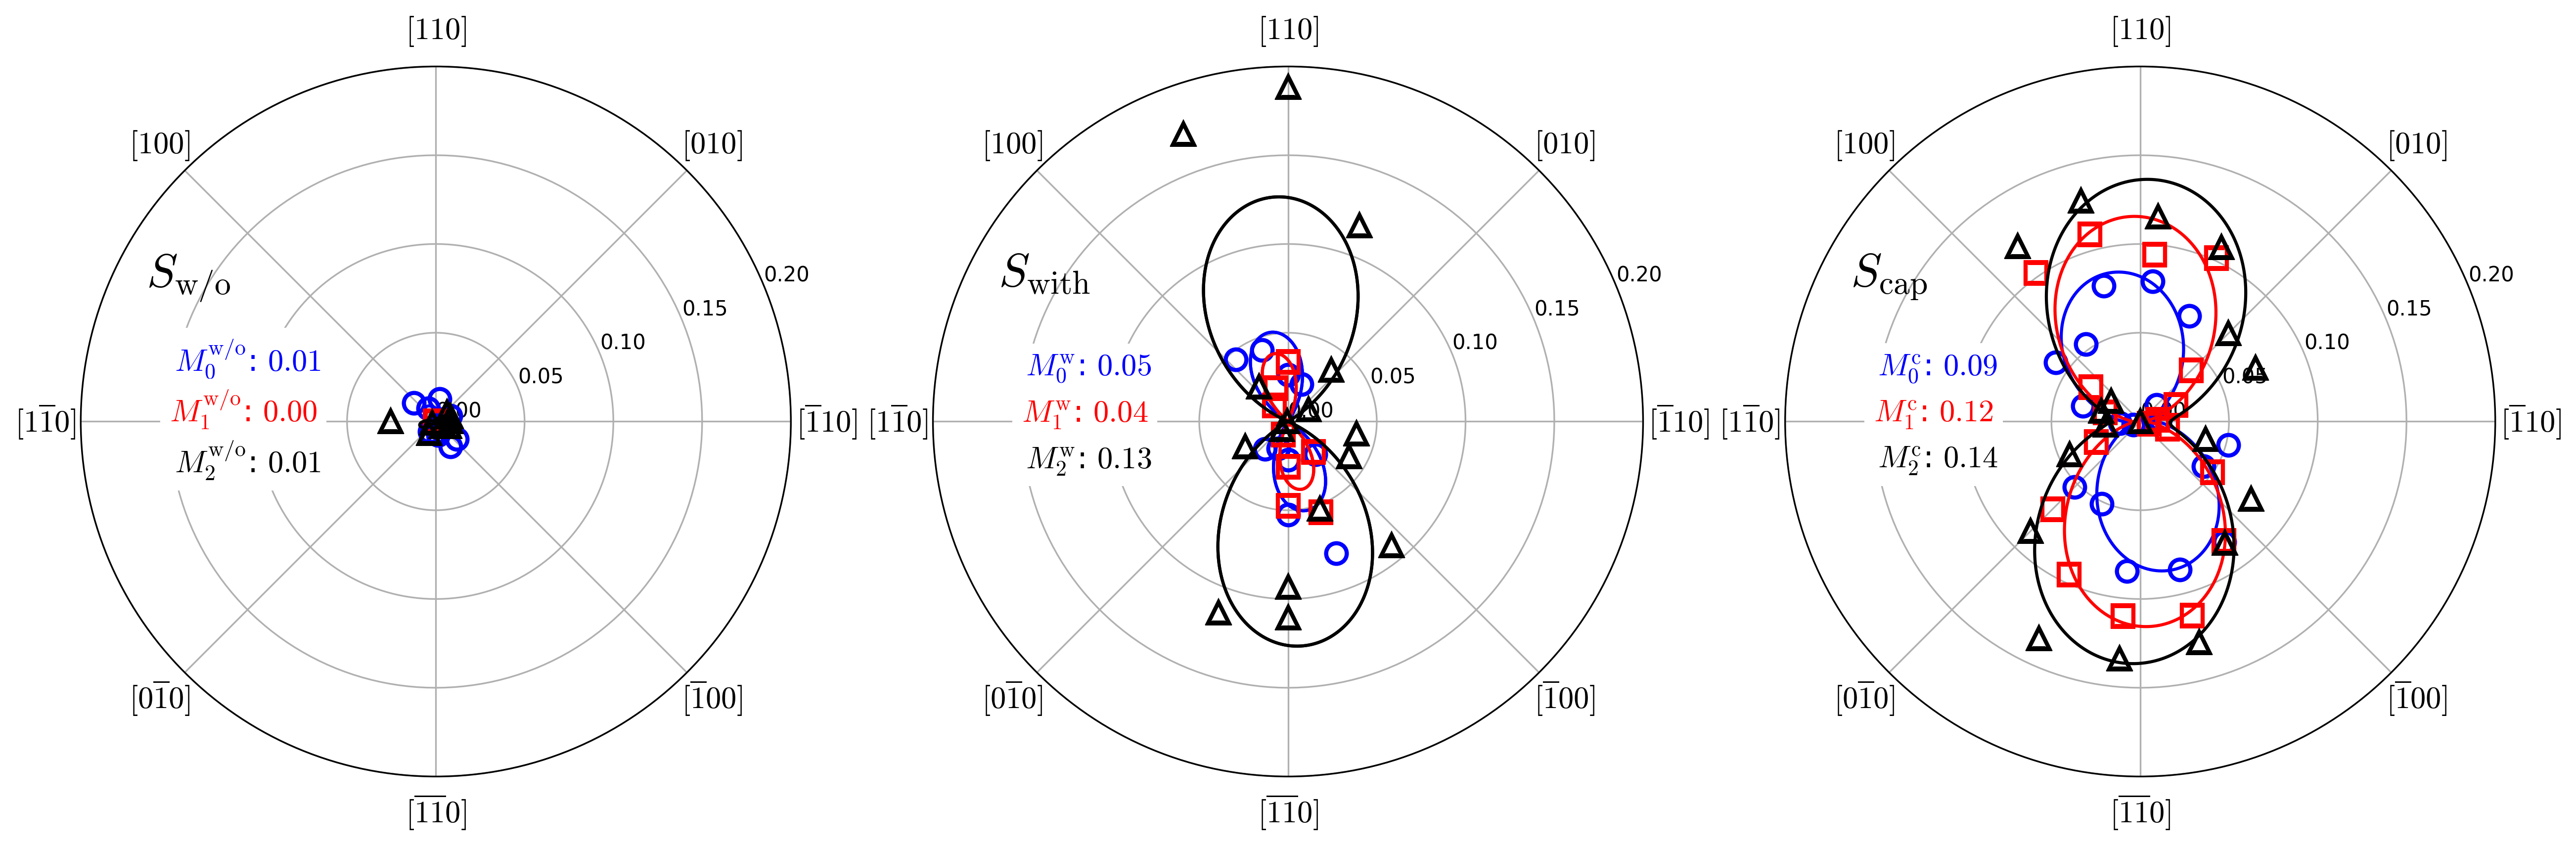
\includegraphics[width=1\linewidth]{/PL/polarization/POL_all}
	\caption{From left to right the polar graphs show $C(\theta)$ of sample ${S_\mathrm{w/o}}$, ${S_\mathrm{with}}$ and $\mathbf{S_\mathrm{cap}}$, respectively. Individual bands of PL spectra for each sample are represented by different symbols, consistently with previous labeling.}
	\label{fig:PL_pol_all}
\end{figure}

\newpage
\section{Time-resolved photoluminiscence}
%The measurements can be fitted to a double exponential decay function after convolution with the instrument response function (IRF) shown in the same graph
We have studied the dynamics of the recombination processes of our QD samples as a function of the emission energy, excitation density, and temperature. Each measured TRPL of $S_\mathrm{w/o}$ signal has been deconvoluted using a double mono-exponential (2ME) decay model
%
\begin{equation}
I(t)=A_1\exp(-t/\tau_1)+A_2\exp(-t/\tau_2),
\end{equation}
 %
 characterized by the amplitude $A_1$ ($A_2$) and the decay time $\tau_1$ ($\tau_2$) for the slow (fast) decay process.
 To reproduce TRPL signal in a maximum of PL intensity of samples $S_\mathrm{w}$ and $S_\mathrm{cap}$ triple mono-exponential (3ME) decay model was used.
 In order to compare the samples we introduce characteristic PL decay time $\tau_\mathrm{PL}$ as the weighted arithmetic mean of two (three) decay times for 2ME (3ME) model which corresponds to a decrease of PL intensity from its maximum value to the level of $1/\mathrm{e}$:
%
\begin{eqnarray}
\tau_\mathrm{PL}=\sum_{i=1}^{2 ( 3) } w_i\tau_i \label{eq:average_time}
\end{eqnarray}
%
where $w_i$ is weight [$w_i={A_i\cdot \tau_i }/{(\sum A_i \cdot \tau_i)}$] defined by fitting model.

Our analysis takes into account repumping of the slow component $\tau_1$ of the dynamics from previous pulses which leads to increase \enquote{background} up to dark signal level as can be seen in Fig.~\ref{fig:TRPL_int_all_max}.


\subsection{Emission energy dependent TRPL}
%

%Using previous analysis the similar fast component $\tau_2$ in range 5 and 13~ns for all samples and $\tau_3$ around 25~ns for $S_\mathrm{w}$ and $S_\mathrm{cap}$ were found.

\begin{figure}[!ht]
	\centering
	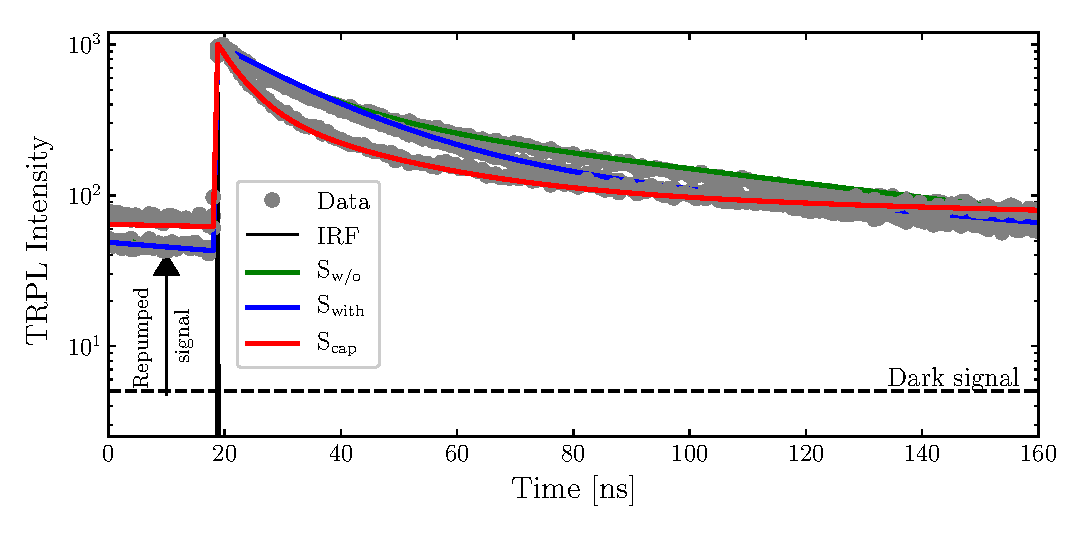
\includegraphics[width=1\linewidth]{/TRPL_after_Benito/intensity/TRPL_inMAX}
	\caption{Comparison of TRPL signal of our samples in their maximum of PL intensity (grey circles) with corresponding multi-exponential fits (solid lines). The black line IRF represents laser scatter. Signal repumped from previous excitation pulses increases \enquote{background} from dark level (dashed line).}
	\label{fig:TRPL_int_all_max}
\end{figure}


In spite of similarity between our samples in $\tau_2$ of values in range 13 and 32~ns (for all samples) and $\tau_3$ smaller than 10~ns (only for $S_\mathrm{with}$ and $S_\mathrm{cap}$), $\tau_1$ of differs from 90~ns ($S_\mathrm{w/o}$) to 520~ns ($S_\mathrm{cap}$). To compare lifetimes across samples and emission energy where weights and number of mono-exponential decays varied, we use $\tau_\mathrm{PL}$. On the one hand, $\tau_\mathrm{PL}$ enlarges within one sample of decreasing energy, see Fig.~\ref{fig:TRPL_int_all}(a) where $\tau_\mathrm{PL}$ measured under the same conditions as a function of the emission energy for all three samples is summarized. On the second hand, that increases between samples from 74~ns ($S_\mathrm{w/o}$), over 164~ns ($S_\mathrm{with}$) to 364~ns ($S_\mathrm{cap}$). Decay times and appropriate weights of multi-exponential fits in the maximum of PL emission of each sample visualized in Fig.~\ref{fig:TRPL_int_all_max} are listed in Tab.~\ref{tab:TRPL_int_params}.
%
\begin{table}
	\centering
	\caption{Summary of the multi-exponential fitting parameters of our samples in the maximum of PL intensity.}
	\begin{tabularx}{0.9\textwidth}{cCCcc}
		\toprule
		sample & $\tau_1/w_1$ [ns/\%]&  $\tau_2/w_2$ [ns/\%]  & $\tau_3/w_3$ [ns/\%] & $\tau_\mathrm{PL}$ [ns] \\ 	
		\midrule
		\midrule
		$S_\mathrm{w/o}$& 91.42/77 & 13.23/23 & -& 73.7\\
		\midrule
		$S_\mathrm{with}$& 360.7/41 &  32.20/46 &9.76/13&  164.0\\
		\midrule
		$S_\mathrm{cap}$ & 518.8/69 &  23.11/21 &4.91/10&  363.7\\ 	
		\bottomrule
	\end{tabularx}\label{tab:TRPL_int_params}
\end{table}
%
%
%
\begin{figure}[!ht]
\centering
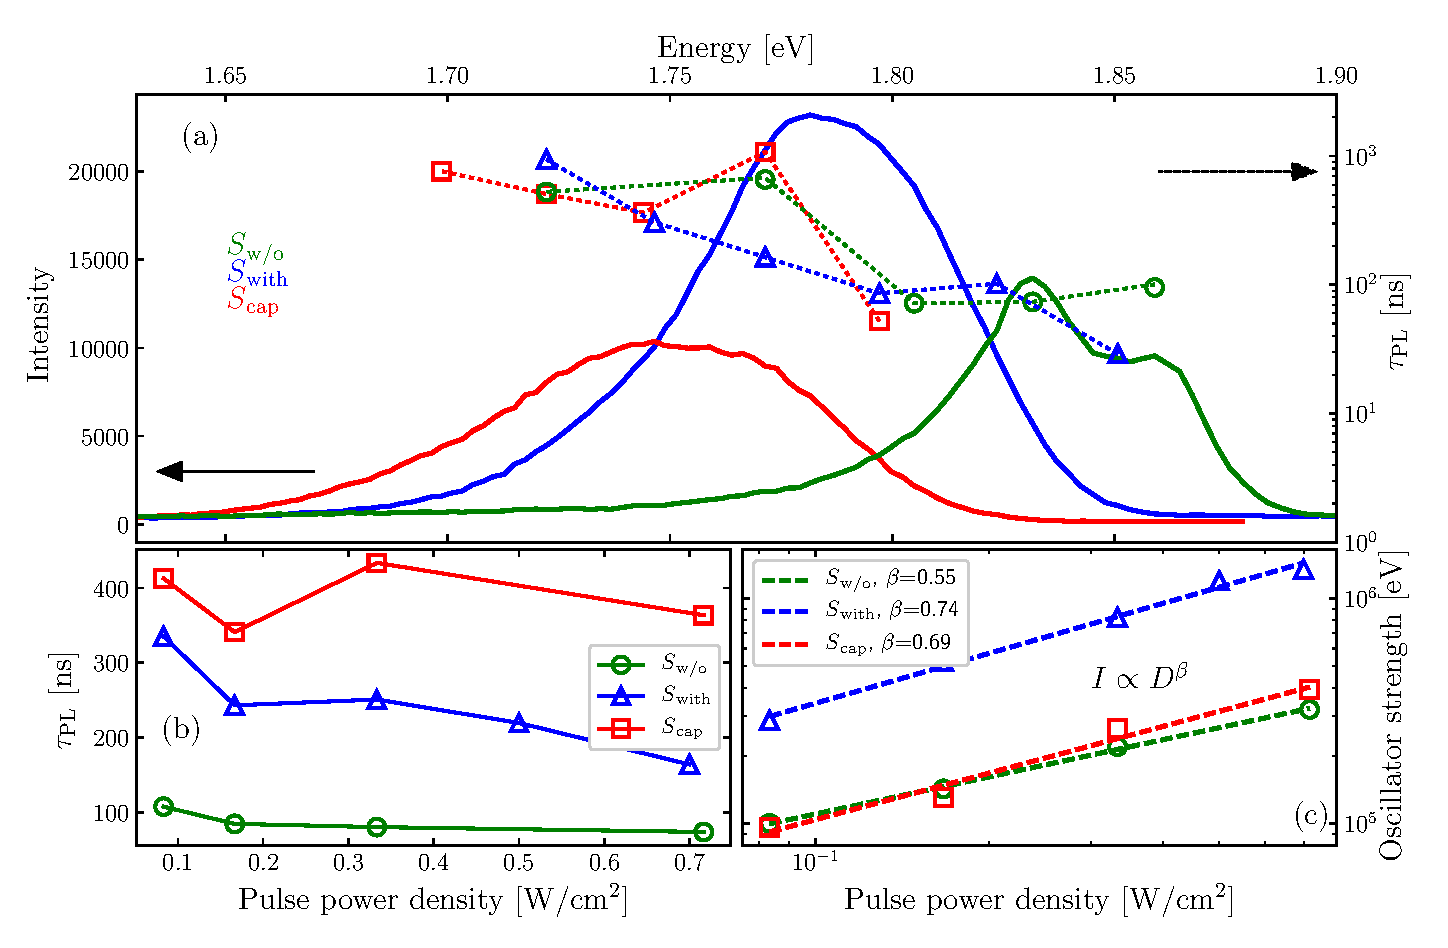
\includegraphics[width=1\linewidth]{/TRPL_after_Benito/intensity/porovnani_vzorku_maximum_int_after_Benito_log}
\caption{(a) Decay times $\tau_\mathrm{PL}$ (symbols) for the studied samples as a function of the emission energy measured at 15~K and 0.7~W/cm$^2$. Appropriate PL spectra (solid lines) are added for better orientation. Panel~(b) depicts $\tau_\mathrm{PL}$ in the maximum of the PL signal and panel~(c) $\tau_\mathrm{PL}$ for the integrated PL intensity in whole measured range as a function of excitation density for the samples.}
\label{fig:TRPL_int_all}
\end{figure}




\newpage
\subsection{Excitation intensity dependent TRPL}
The excitation density of the pulse laser was varied in the range 0.08--0.7~W/cm$^2$ (the optical response was in linear regime in the whole varied excitation range for each sample, see Fig.~\ref{fig:TRPL_int_all}(c)), then the measured TRPL signal has been deconvoluted by multi-exponential decay model. %, e.~g., Fig.~\ref{fig:TRPL_int_w} depicts TRPL signal in the maximum of PL spectra of $S_\mathrm{with}$). 

Let's start with TRPL of sample $S_\mathrm{w/o}$ depicted in Fig.~\ref{fig:TRPL_int_wo} where a decrease of decay times were observed, $\tau_1$ from 130 to 90~ns and $\tau_2$ from 30 to 13~ns.
The decrease of decay times point to indirect transition electrons from X band to heavy holes in $\Gamma$ band in GaAs, moreover weight of the processes stay same which can be connected with character of $M_1^\mathrm{w/o}$ and $M_2^\mathrm{w/o}$, where in Sec.~\ref{Sec:PL_int_wo} was discussed, that $M_1^\mathrm{w/o}$ is phonon replica of $M_2^\mathrm{w/o}$. (Je to dobre s tim typem II v rec. prostoru?)

%This behaviour arrived us to Because the faster process $\tau_2$ was observed across our samples and emission energy, we assume that it comes from the substrate. (Je to dobre s tim typem II v rec. prostoru?)

%We observe a decrease of the fast decay component with increasing excitation density as shown in Fig.~\ref{fig:TRPL_int_w}(b)--(c), which is in agreement with behaviour of type-II nanostructures observed elsewhere~\citep{Ledentsov_prb1995_intmodel,Gu_prb2005_TRPLtype2,Manna_apl2012_TRPLtype2,Zaitsev_prb2007}. At higher excitation intensity, a larger carrier concentration of the photogenerated electron-hole pairs results in band bending, hence a stronger overlap of electron-hole wave-functions, and thus a faster decay.
%

\begin{figure}
	\centering
	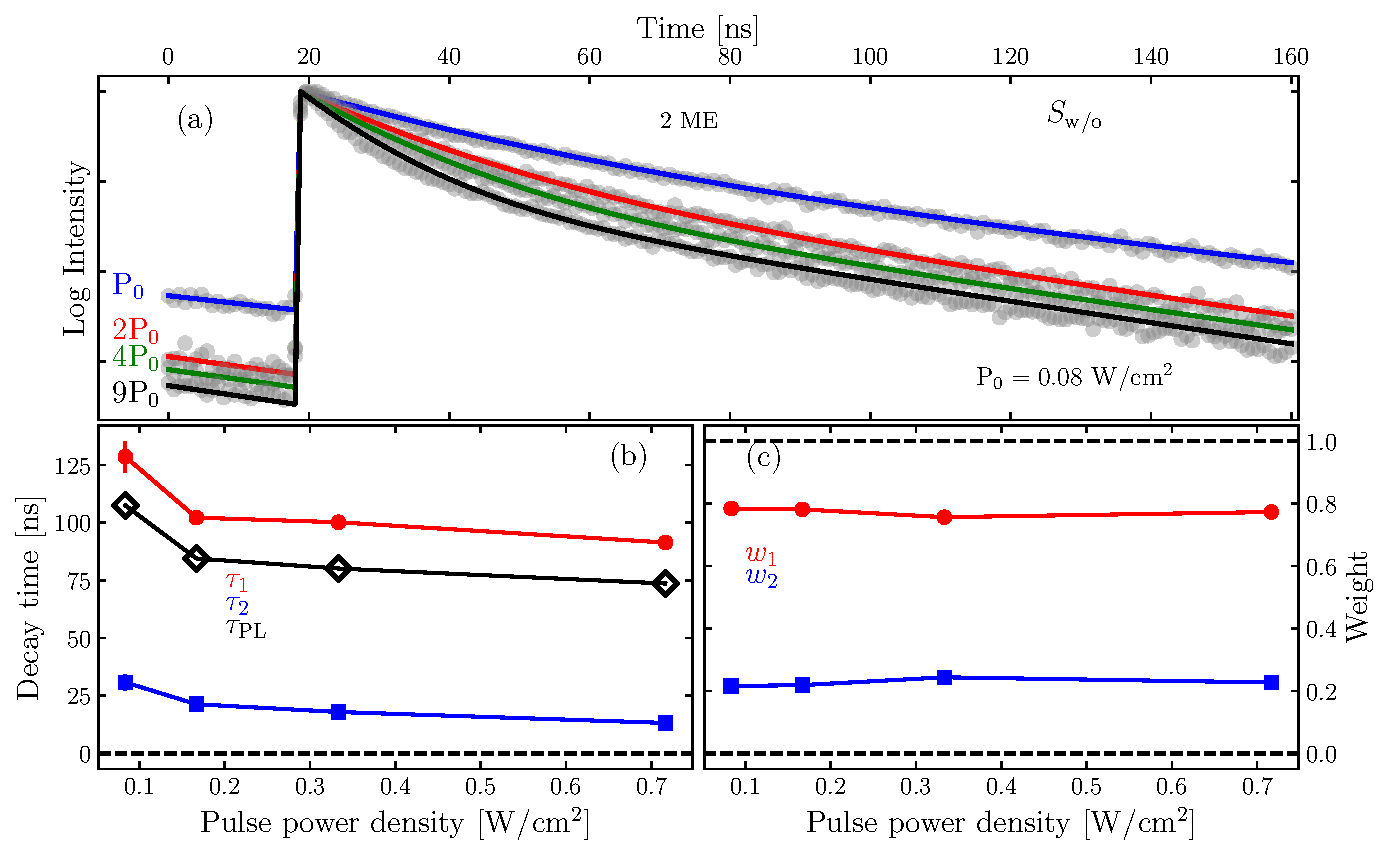
\includegraphics[width=1\linewidth]{/TRPL_after_Benito/intensity/12027_TRPL_677nm_int}
	\caption{(a) Experimental TRPL measured at 15~K as a function of excitation density (grey circles) and its deconvolution by 2ME model (solid lines) at the maximum of band $M^1_\mathrm{w/o}$ for sample $S_\mathrm{w/o}$. (b) Fitted decay times $\tau_1$ (red circles), $\tau_2$ (blue squares) and characteristic time $\tau_\mathrm{PL}$ (black stars) as a function of excitation density. Appropriate weights are shown in panel (c).}
	\label{fig:TRPL_int_wo}
\end{figure}

%Samples $S_\mathrm{with}$ and $S_\mathrm{cap}$ were fitted by 3ME model with very similar behaviour of $\tau_2$ as in sample $S_\mathrm{w/o}$, i.~e., a slight decrease in decay times and the same difference in weights. Moreover, $\tau_2$ is in range between 20 and 35~ns which is comparable with $\tau_2$ in $S_\mathrm{w/o}$. But, interestingly, $\tau_1$ is independent on excitation intensity or slightly increasing with that for both $S_\mathrm{with}$ and $S_\mathrm{cap}$ samples and it is much longer than other decay times: $\tau_1$ is between 330~ns (450~ns) and 380~ns (540~ns) for $S_\mathrm{with}$ ($S_\mathrm{cap}$). 


Samples $S_\mathrm{with}$ and $S_\mathrm{cap}$ were fitted by 3ME model with very similar behaviour of $\tau_2$ as in sample $S_\mathrm{w/o}$, i.~e., a slight decrease in decay times from 35 to 30 for $S_\mathrm{with}$ or 25 to 20~ns for $S_\mathrm{cap}$, respectively, which is comparable with $\tau_2$ in $S_\mathrm{w/o}$.
%
The processes characterized by $\tau_1$ and $\tau_3$ are presented only on samples $S_\mathrm{with}$ and $S_\mathrm{cap}$ stay almost constant ($\tau_3=8$~ns) or only slightly increase ($\tau_1$) with increasing excitation power which is behaviour observed for type-I nanostructures. (máš nějakou referenci, ja nemuzu nic najit)

%Process characterized by $\tau_3$ is presented only on samples $S_\mathrm{with}$ and $S_\mathrm{cap}$ and stays constant with increasing excitation power at 8~ns.

Interestingly, the third process characterized by $\tau_1$ is independent on excitation intensity or slightly increasing with that for both $S_\mathrm{with}$ and $S_\mathrm{cap}$ samples and it is much longer than other decay times: $\tau_1$ is between 330~ns (450~ns) and 380~ns (540~ns) for $S_\mathrm{with}$ ($S_\mathrm{cap}$). 

These processes characterized by decay times $\tau_1$ and $\tau_3$ and their evolutions with intensity of excitation laser were simulated using SSCCI by the supervisor. The process with $\tau_1$ was identified as a radiative transition between electrons originating from $L$ and holes from $\Gamma$-point. On the other hand, a radiative transition from $\Gamma$ electrons can describe the process characterized by $\tau_3$. For comparison SSCCI calculations and experimental obtained decay times as a function of excitation power see Fig.~\ref{fig:TRPL_int_c_theory}.
\begin{figure}
	\centering
	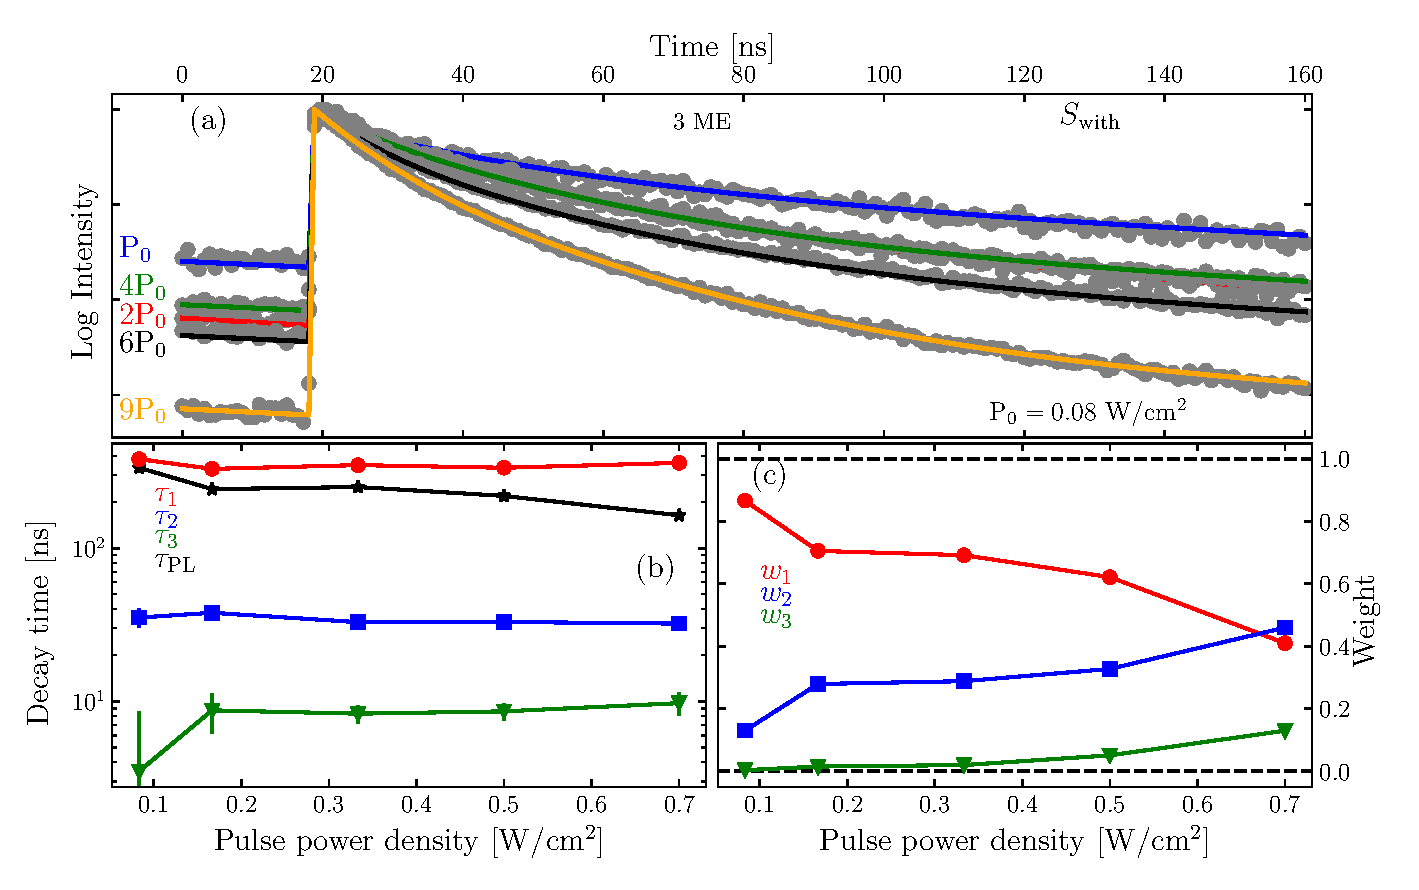
\includegraphics[width=1\linewidth]{/TRPL_after_Benito/intensity/12040_TRPL_700nm_int}
	\caption{(a) Deconvolved TRPL signal measured at 15~K by 3ME (solid lines) as a function of excitation density (grey circles) at the maximum of band $M_1^\mathrm{w}$ for sample $S_\mathrm{with}$. (b) Fitted decay times $\tau_1$ (red circles), $\tau_2$ (blue squares), $\tau_3$ (green triangles) and characteristic time $\tau_\mathrm{PL}$ (black stars) as a function of excitation density. Appropriate weights are shown in panel (c).}
	\label{fig:TRPL_int_w}
\end{figure}

\begin{figure}
	\centering
	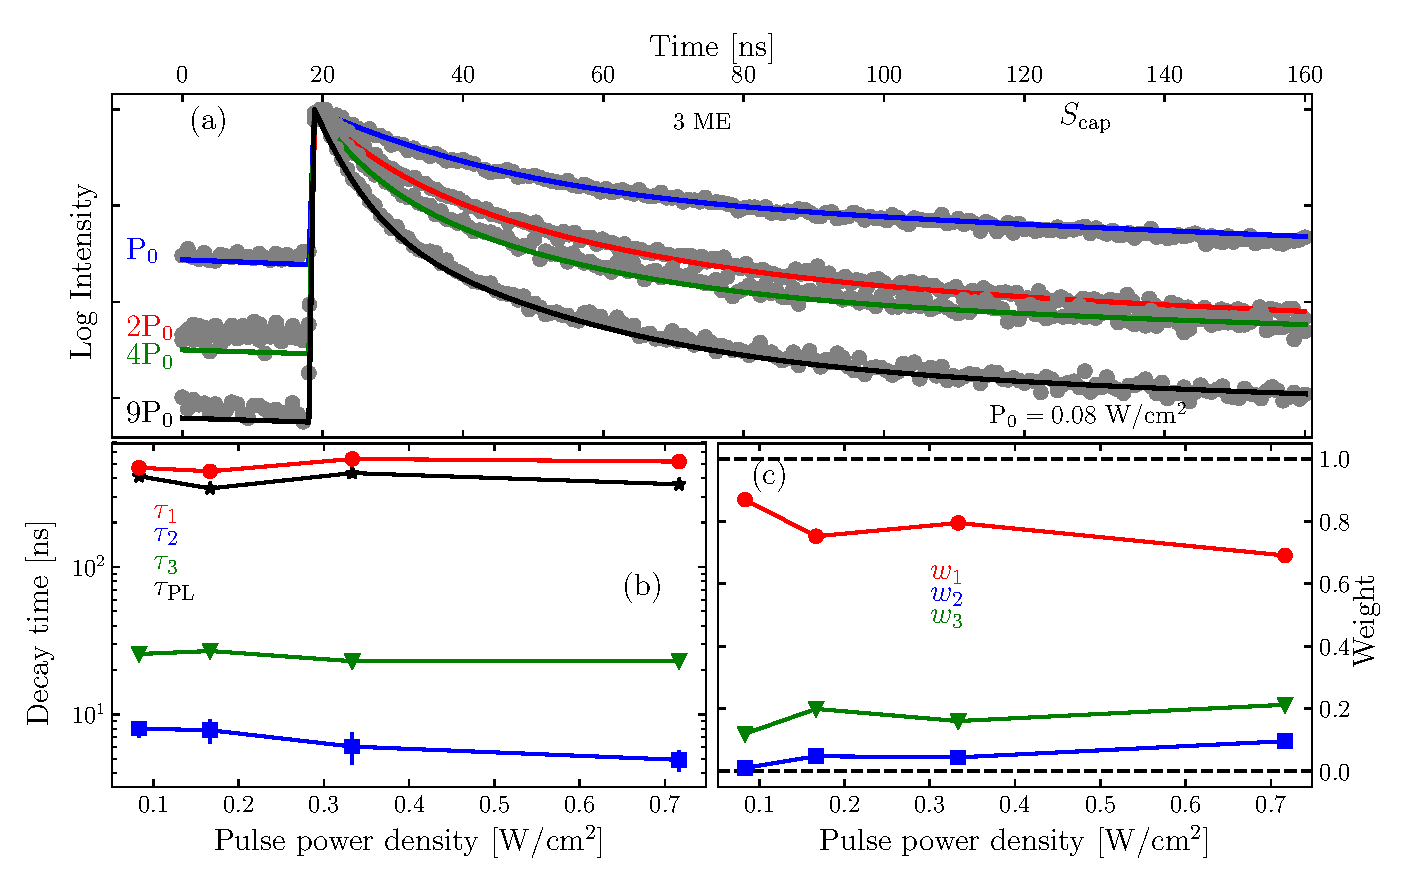
\includegraphics[width=1\linewidth]{/TRPL_after_Benito/intensity/12021_TRPL_710nm_int}
	\caption{TRPL signal of $S_\mathrm{cap}$ deconvoluted similarly as in Fig.~\ref{fig:TRPL_int_w}.}
	\label{fig:TRPL_int_c}
\end{figure}


\begin{figure}
	\centering
	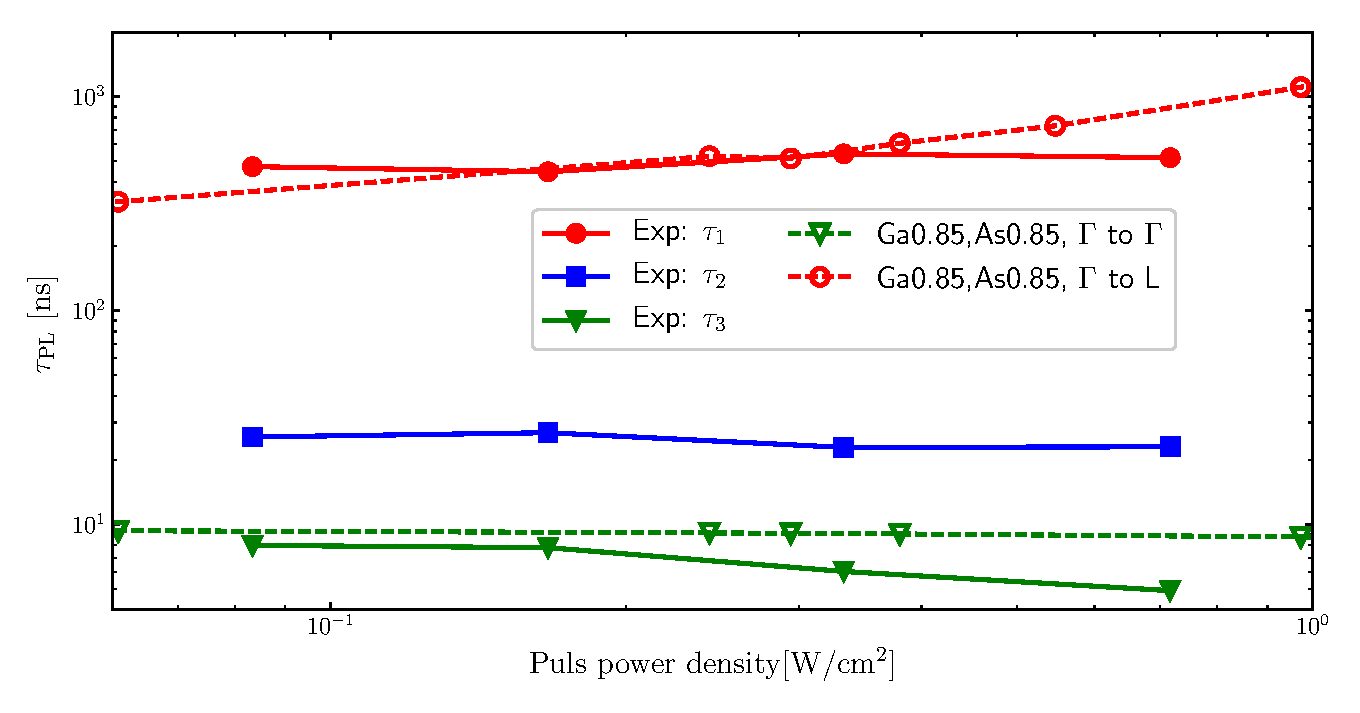
\includegraphics[width=1\linewidth]{/TRPL_after_Benito/intensity/12040_1107_TRPL_int_vs_theory_LandGamma}
	\caption{Experimental decay times obtained by 3ME fit of TRPL signal of $S_\mathrm{cap}$ (fill symbols) as a function of excitation intensity and SSCCI with single-particle bases calculated by $1\times8$ $\mathbf{k\cdot p}$ and $8\times8$ $\mathbf{k\cdot p}$ (dashed lines).}
	\label{fig:TRPL_int_c_theory}
\end{figure}

%Other samples given in appendix~\ref{chapter:appendix_TRPL_int} show similar behaviour and with comparable $\tau_\mathrm{PL}$ at low excitation power. However, $\tau_\mathrm{PL}$ of samples with QDs is approximately twice as small, see Fig.~\ref{fig:TRPL_int_all}(b).

\newpage
\subsection{Temperature dependent TRPL}
TRPL variations with temperature are shown in Figs.~\ref{fig:TRPL_temp_wo}-\ref{fig:TRPL_temp_c} and are deconvoluted again by 2ME model. As it can be seen in Fig.~\ref{fig:TRPL_temp_w}, the resulting decay times of sample $S_\mathrm{with}$ increase up to the temperature of 30~K and then progressively reduce which is characteristic of the appearance of thermally activated scape paths~\citep{Manna_apl2012_TRPLtype2}. Contrary to sample $S_\mathrm{with}$, on $S_\mathrm{w/o}$ and $S_\mathrm{cap}$ the reduction of the decay times begins at the lowest temperatures without an increase at the beginning.
%
\begin{figure}
	\centering
	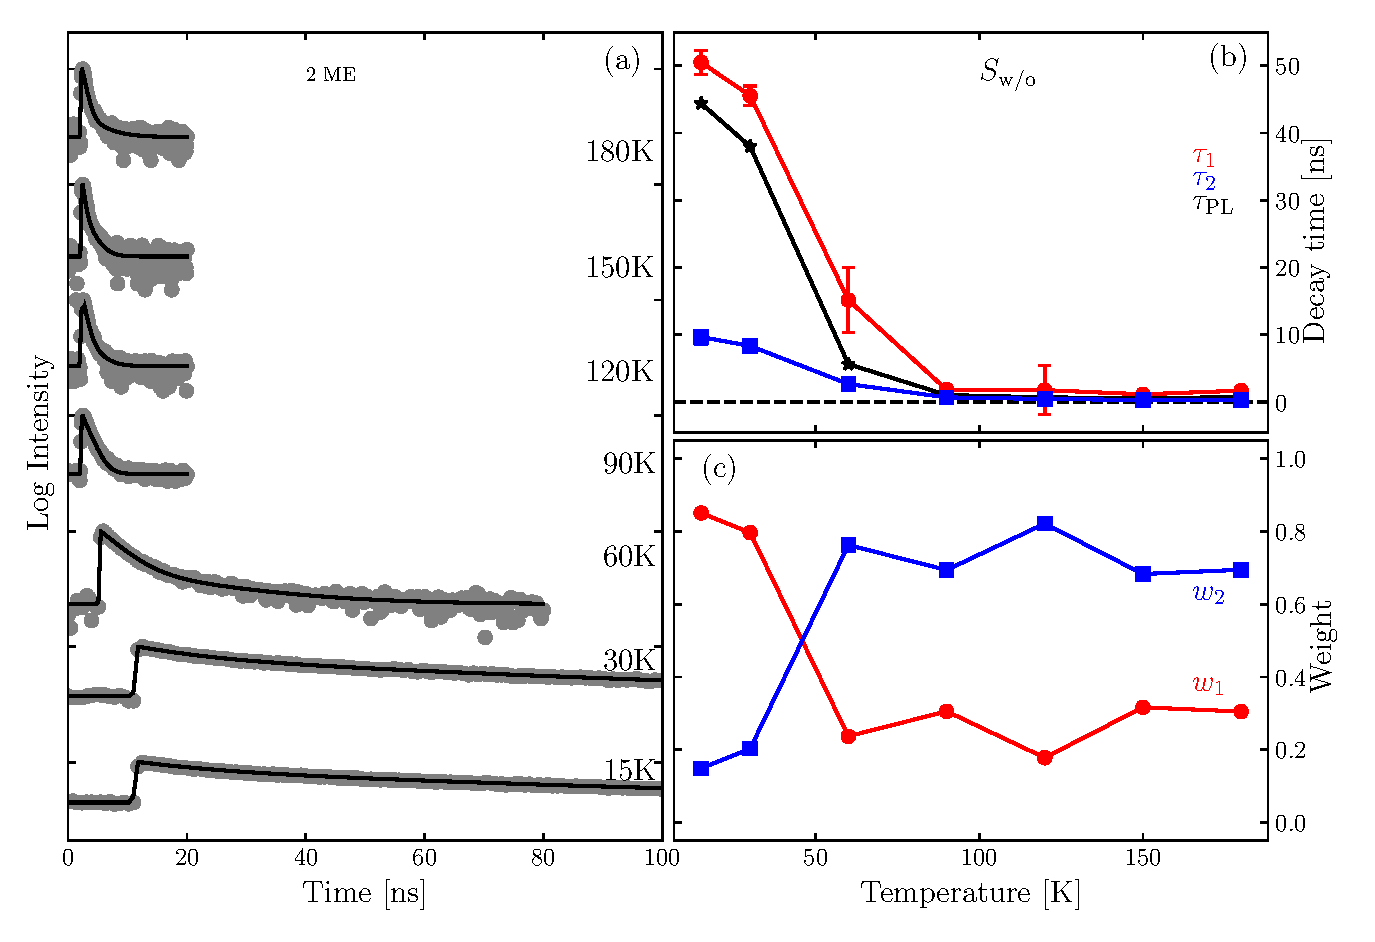
\includegraphics[width=0.9\linewidth]{/TRPL/temperature/12027_TRPL_max677_temp}
	\caption{(a) Experimental TRPL at pumping power of 0.3~W/cm$^2$ as a function of temperature (grey circles) and its deconvolution by 2ME model (solid black lines) at the maximum of PL signal in sample $S_\mathrm{w/o}$. (b) Deconvolved decay times ($\tau_1$: red circles; $\tau_2$: blue squares) and characteristic time $\tau_\mathrm{PL}$ (black stars) as a function of temperature. Corresponding weights are shown in panel (c).}
	\label{fig:TRPL_temp_wo}
\end{figure}
%
\begin{figure}
	\centering
	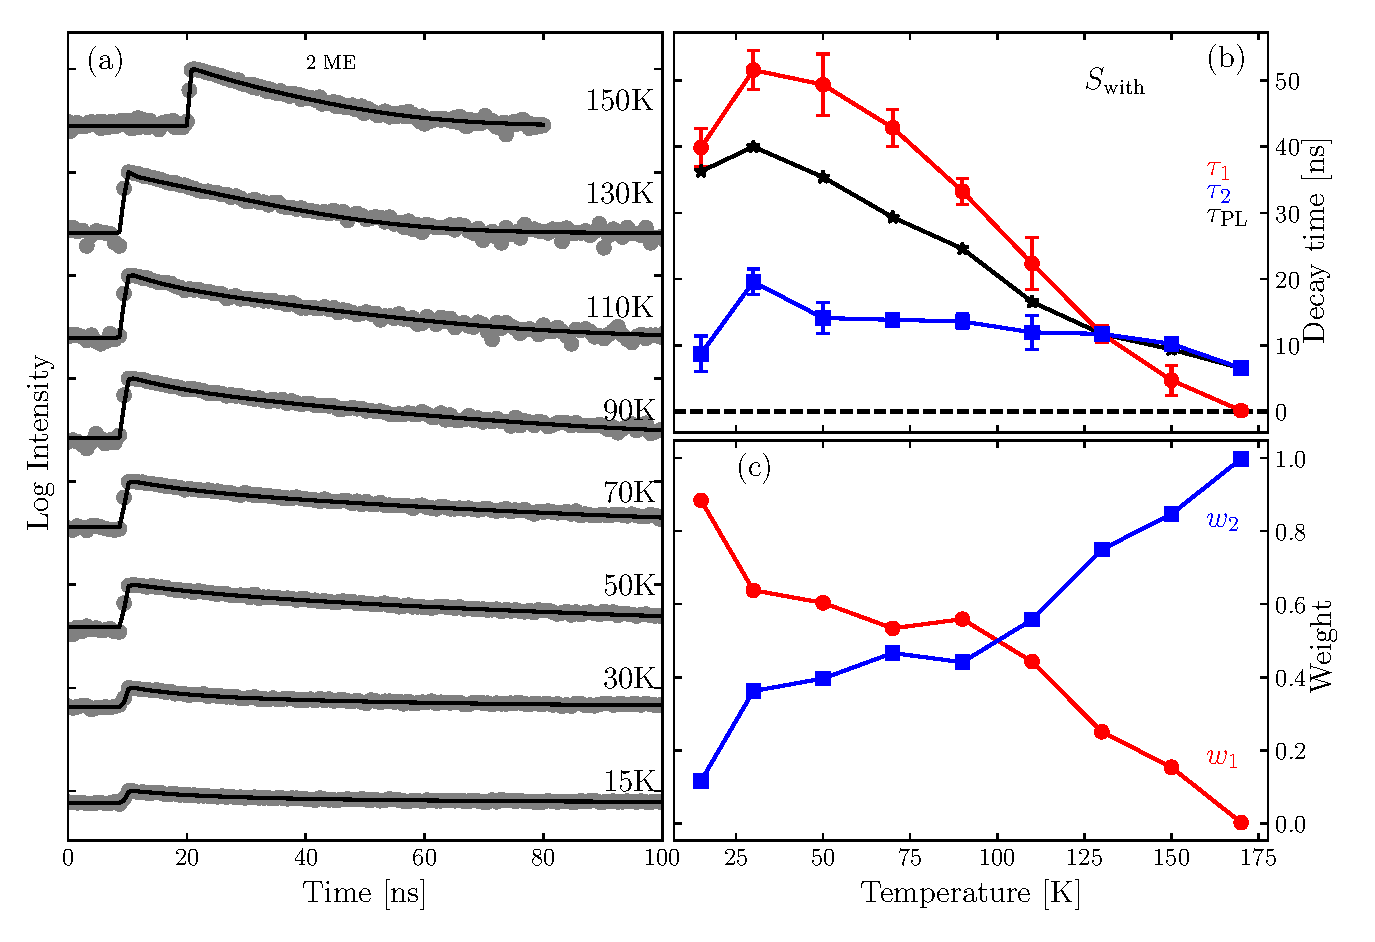
\includegraphics[width=0.9\linewidth]{/TRPL/temperature/12040_TRPL_700-710_temp}
	\caption{TRPL signal as a function of temperature at the maximum of PL in sample $S_\mathrm{with}$ similarly commented as in Fig.~\ref{fig:TRPL_temp_wo}.}
	\label{fig:TRPL_temp_w}
\end{figure}
%

If we assume similarly as in Ref.~\citep{t_alvarez} that at 15~K the only loss mechanism is radiative recombination, the radiative $\tau_\mathrm{R}$ and non-radiative $\tau_\mathrm{NR}$ decay times can be extracted from $\tau_\mathrm{PL}$ by
%
\begin{equation}
\tau_\mathrm{R}=\frac{I_0}{I_\mathrm{PL}(T)}\tau_\mathrm{PL} \label{eq:tau_R_fromPL}
\end{equation}
and
\begin{equation}
\frac{1}{\tau_\mathrm{PL}}=\frac{1}{\tau_\mathrm{R}} + \frac{1}{\tau_\mathrm{NR}}
\end{equation}
%
\begin{figure}
	\centering
	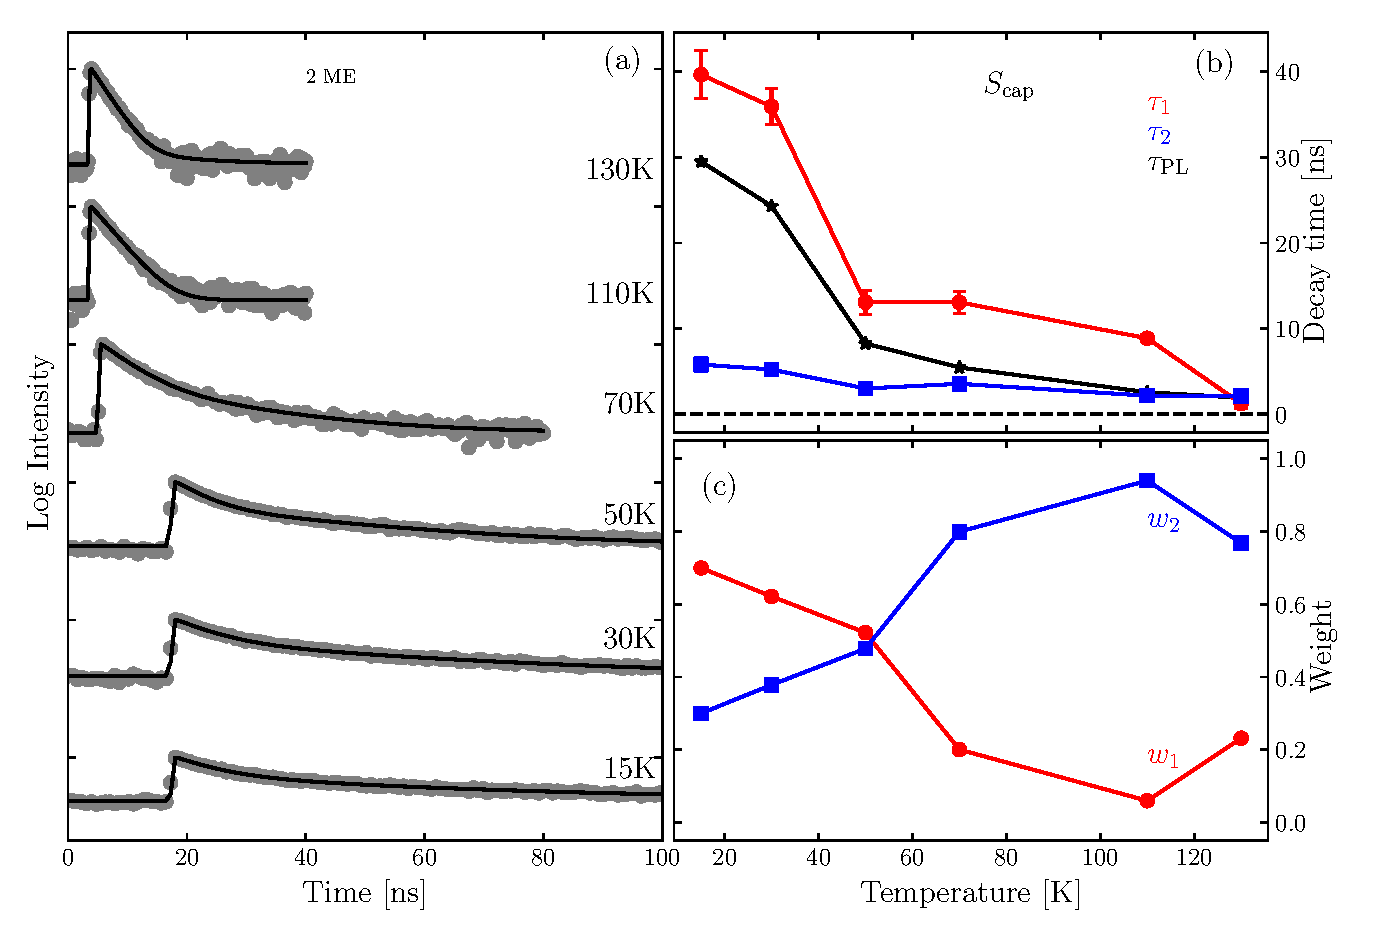
\includegraphics[width=0.9\linewidth]{/TRPL/temperature/12021_TRPL_690_temp}
	\caption{TRPL signal as a function of temperature at the maximum of PL in sample $S_\mathrm{cap}$ similarly commented as in Fig.~\ref{fig:TRPL_temp_wo}.}
	\label{fig:TRPL_temp_c}
\end{figure}
%

\noindent where $I_0$ and $I_\mathrm{PL}$ are the PL intensity at 15~K and that as a function of $T$, respectively. As can be seen in Fig.~\ref{fig:TRPL_temp_decon} $\tau_\mathrm{NR}$ decreases with temperature as is usually the case for thermally activated processes. Parameter $\tau_\mathrm{NR}$ can be fitted with two non-radiative processes 
%
\begin{equation}
\frac{1}{\tau_\mathrm{NR}}=\frac{1}{\tau_\mathrm{NR}^1}\exp{\left(\frac{-E_1}{k_\mathrm{B}T}\right)} + \frac{1}{\tau_\mathrm{NR}^2}\exp{\left(\frac{-E_2}{k_\mathrm{B}T}\right)} \label{eq:nonradiative}
\end{equation}
characterized by activation energies $E_1$ and $E_2$ and time constants $\tau_\mathrm{NR}^1$ and $\tau_\mathrm{NR}^2$, respectively.
Conversely, $\tau_\mathrm{R}$ increases exponentially with temperature
%
\begin{equation}
\tau_\mathrm{R} = \tau_\mathrm{R}^0 + \tau_\mathrm{R}^T \exp{\left(\frac{T}{T_C}\right)}, \label{eq:tau_R} 
\end{equation}
where $ \tau_\mathrm{R}^0$ ($ \tau_\mathrm{R}^T$) describes the temperature independent (dependent) part of the radiative decay and $T_C$ is the characteristic temperature corresponding to the energy of localized states. Inserting Eq.~(\ref{eq:tau_R_fromPL}) into Eq.~(\ref{eq:tau_R}) we can obtain an Arrhenius-like equation with an explicit dependence of the PL intensity on all the parameters derived from the TRPL analysis
%
\begin{equation}
I_\mathrm{PL}(T)=\frac{I_0}{1+\left[\tau_\mathrm{R}^0+\tau_\mathrm{R}^T\exp{\left(\frac{T}{T_C}\right)}\right] \times \left[\frac{1}{\tau_\mathrm{NR}^1}\exp{\left(\frac{-E_1}{k_\mathrm{B}T}\right)} + \frac{1}{\tau_\mathrm{NR}^2}\exp{\left(\frac{-E_2}{k_\mathrm{B}T}\right)}\right]}. \label{eq:TRPL_Arhenius}
\end{equation}
%
\begin{figure}
	\centering
	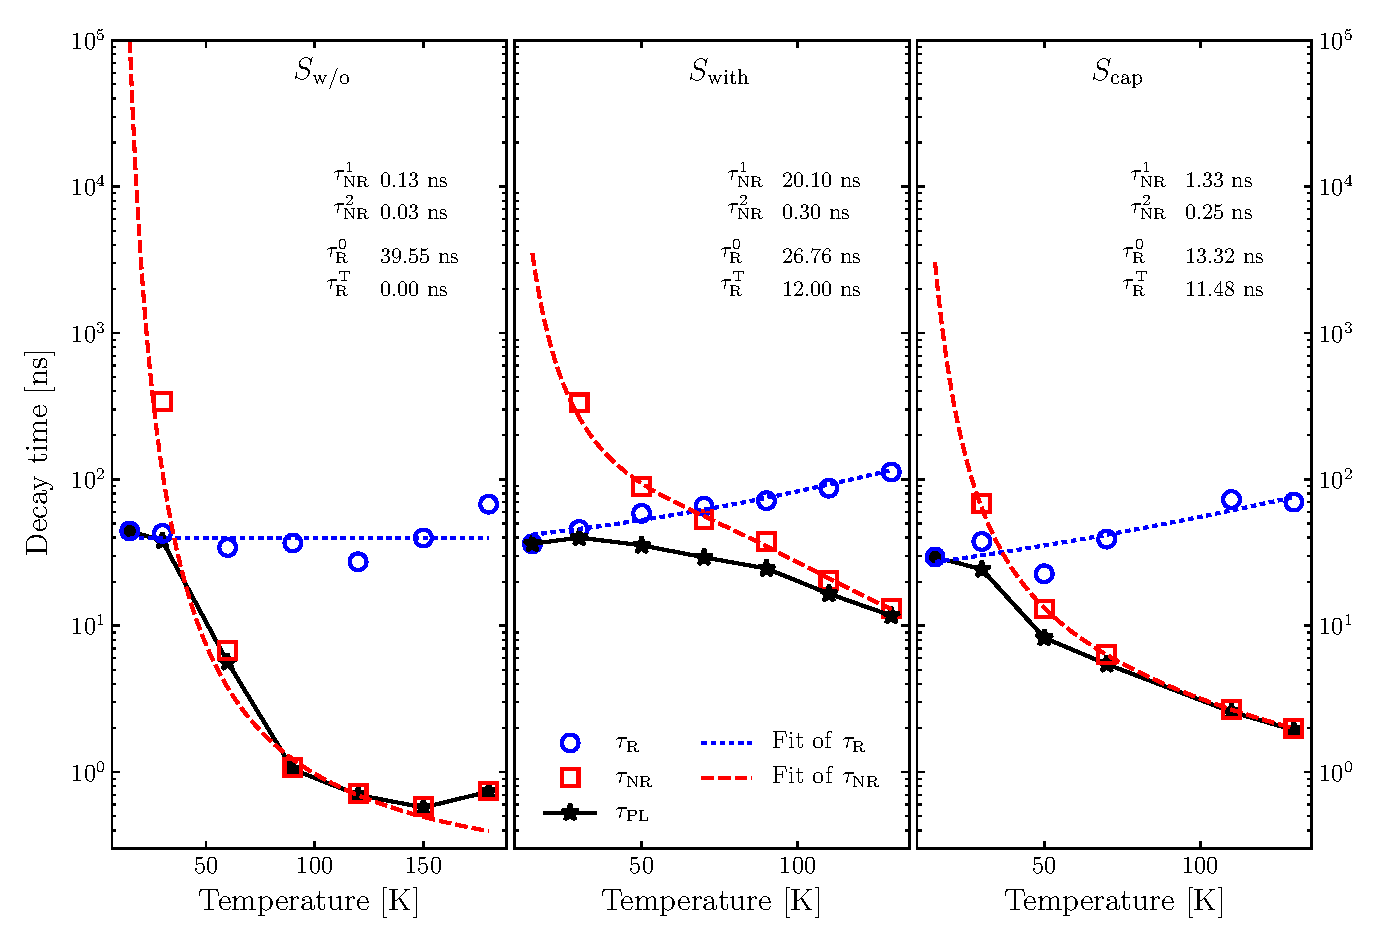
\includegraphics[width=1\linewidth]{/TRPL/temperature/decay_dekonvolution_all}
	\caption{Characteristic PL decay time $\tau_\mathrm{PL}$ as a function of temperature with the radiative and non-radiative components for all our samples. The radiative and non-radiative component are fitted by Eq.~(\ref{eq:tau_R}) and Eq.~(\ref{eq:nonradiative}), respectively.}
	\label{fig:TRPL_temp_decon}
\end{figure}

As it can be seen in Fig.~\ref{fig:Arrhenius_PLandTRPL}, this formula is equally good in reproducing experimental data as~Eq.~(\ref{eq:Arhenius}). 


\newpage

We now discuss the numerical results obtained in this analysis that are summarized in Tab.~\ref{tab:TRPL_params}. As can be seen in Fig.~\ref{fig:TRPL_temp_decon} the radiative decay time of $S_\mathrm{w/o}$ does not depend on temperature and is described only by $\tau_\mathrm{R}^0=39.6$~ns. On the contrary, the radiative decay time of samples with QDs exponentially grows with temperature and is proportional to similar value, i.~e., $\tau_\mathrm{R}^T=12.0$~ns for $S_\mathrm{with}$ and $11.5$~ns for $S_\mathrm{cap}$, respectively. 
The non-radiative process with smaller activation energy ($E_1$ between 6 and 18~meV) is probably associated with trapping of carriers by impurities or defects in the vicinity of QDs, as it has been also before for InAs/InP quantum wires~\citep{Alen_apl2011}. The other process is characterized by faster time constant $\tau_\mathrm{NR}^2$ ($\tau_\mathrm{NR}^1/\tau_\mathrm{NR}^2>5$) is close to the thermally activated capture of excitions by nonradiative defects in GaAs layer~\citep{Seravallo_apl2005,Kohki_apl1997}. 

The values obtained by fitting the dependencies by model in Eq.~(\ref{eq:TRPL_Arhenius}) are summarized in Tab.~\ref{tab:TRPL_params} and are comparable with parameters gained from the temperature dependence PL data shown in Sec.~\ref{Sec:temp_PL_TU}, which are equally well reproduced by Eq.~\ref{eq:Arhenius}, see the parameters resume in Tab.~\ref{tab:Arhenius}.

The previous temperature dependent TRPL and PL analysis of the samples allow us to draw simple scheme of the time evolution of the levels involved in the exciton dynamics, namely that of the recombining level \textbf{F} and three trap levels \textbf{N$_i$}, see Fig.~\ref{fig:Arrhenius_PLandTRPL}.
\begin{table}
	\centering
	\caption{Summary of the TRPL Arrhenius-like fits. The displayed values are obtained with accuracy better than $10^{-3}\%$.}
	\begin{tabularx}{0.9\textwidth}{cCCccccc}
		\toprule
		
		 & $E_1$ [meV]& $\tau_\mathrm{NR}^1$ [ns]& $E_2$ [meV]& $\tau_\mathrm{NR}^2$ [ns] & $\tau_\mathrm{R}^0$ [ns]& $\tau_\mathrm{R}^T$ [ns]& $T_C$ [K]\\ 	
		\midrule
		\midrule
		$S_\mathrm{w/o}$& 17.5&0.13&294.3 & 0.03& 39.55&0.00&8825.0\\
		$S_\mathrm{with}$&6.7 & 20.10& 47.2&0.30& 26.76&12.00&64.9\\
		$S_\mathrm{cap}$& 10.0&1.33&33.8 & 0.25& 13.32&11.48&76.9\\
		
		\bottomrule
	\end{tabularx}\label{tab:TRPL_params}
\end{table}



\begin{figure}
	\centering
	\includegraphics[width=0.9\linewidth]{/TRPL/temperature/models} %Arrhenius_PLandTRPL_all}
	\caption{The left panels (a)-(c) compare the integrated PL intensity and the corresponding fit for all our samples of the measurements performed with a CW (circles) and a pulsed (squares) laser. The right panels show levels involved in the exciton dynamics in our samples. The letters \textbf{0} and \textbf{F} in these sketches represent the vacuum end exciton state, respectively, \textbf{N$_i$} are three trap levels.}
	\label{fig:Arrhenius_PLandTRPL}
\end{figure}
\newpage 

\section{Conclusions}
We have experimentally studied the electronic structure of set (without QDs, with QDs, with QDs and GaSb capping) of In$_{1-x}$Ga$_{x}$As$_y$Sb$_{1-y}$/GaP QDs with 5~ML GaAs interlayer grown by MOVPE. We have pointed by TEM and EDX measurements to a high amount of Ga and As in our samples which lead to type-I band alignment. Furthermore, we have shown that the samples emitted around 1.8~eV with anisotropy elongated along [110]~crystallographic direction.   % For our analysis set of sample (without QDs, with QDs, with QDs and GaSb capping) were grown by MOVPE. 

CO DÁL???